\documentclass[%
%%% PARA ESCOLHER O ESTILO TIRE O SIMBOLO %(COMENT�RIO)
%SemVinculoColorido,
%SemFormatacaoCapitulo,
%SemFolhaAprovacao,
%SemImagens,
%CitacaoNumerica, %% o padr�o � cita��o tipo autor-data
PublicacaoDissOuTese, %% (� tamb�m o "default") com ficha catal. e folha de aprova��o em branco. Caso tenha lista de s�mbolos e lista de siglas e abreviaturas retirar os coment�rios dos arquivos siglas.tex e abreviaturasesiglas.tex. Retirar tamb�m os coment�rios indicados nesse arquivo, nos includes
%PublicacaoArtigoOuRelatorio, %% texto sequencial, sem quebra de p�ginas nem folhas em branco
%PublicacaoProposta, %% igual tese/disserta��o, mas sem ficha catal. e fol. de aprov.
%PublicacaoLivro, %% com cap�tulos
%PublicacaoLivro,SemFormatacaoCapitulo, %% sem cap�tulos
english,portuguese %% para os documentos em Portugu�s com abstract.tex em Ingl�s
%portuguese,english %% para os documentos em Ingl�s com abstract.tex em Portugu�s
%,LogoINPE	%% comentar essa linha para fazer aparecer o logo do Governo
]{tdiinpe}
%]{../../../../../iconet.com.br/banon/2008/03.25.01.19/doc/tdiinpe}

% PARA EXIBIR EM ARIAL TIRAR O COMENT�RIO DAS DUAS LINHAS SEGUINTES
%\renewcommand{\rmdefault}{phv} % Arial
%\renewcommand{\sfdefault}{phv} % Arial

% PARA PUBLICA��ES EM INGL�S:
% renomear o arquivo: abnt-alf.bst para abnt-alfportuguese.bst
% renomear o arquivo: abnt-alfenglish.bst para abnt-alf.bst


%%%%%%%%%%%%%%%%%%%%%%%%%%%%%%%%%%%%%%%%%%%%%
%%% Pacotes j� previamente carregados:      %
%%%%%%%%%%%%%%%%%%%%%%%%%%%%%%%%%%%%%%%%%%%%%%%%%%%%%%%%%%%%%%%%%%%%%%%%
%%% ifthen,calc,graphicx,color,inputenc,babel,hyphenat,array,setspace, %
%%% bigdelim,multirow,supertabular,tabularx,longtable,lastpage,lscape, %
%%% rotate,caption2,amsmath,amssymb,amsthm,subfigure,tocloft,makeidx,  %
%%% eso-pic,calligra,hyperref,ae,fontenc                               %
%%%%%%%%%%%%%%%%%%%%%%%%%%%%%%%%%%%%%%%%%%%%%%%%%%%%%%%%%%%%%%%%%%%%%%%%
%%% insira neste campo, comandos de LaTeX %%%
%%% \usepackage{_exemplo_}
% etc.
%%%%%%%%%%%%%%%%%%%%%%%%%%%%%%%%%%%%%%%%%%%%%

%\watermark{Revis�o No. *00*} %% use o comando \watermark para identificar a vers�o de seu documento
%% comente este comando quando for gerar a vers�o final
\usepackage{rotating}
\usepackage{dsfont}
\usepackage{comment}
\usepackage{blindtext}
%\usepackage{todonotes}
\usepackage{ulem}
\usepackage{enumerate}
\usepackage{booktabs}
\usepackage{lscape}
\usepackage{multicol}
%\usepackage{todo}
\usepackage[export]{adjustbox}% http://ctan.org/pkg/adjustbox
%\usepackage{enumitem}
\usepackage{booktabs}
\usepackage{enumitem}
\usepackage{pdflscape}
\usepackage{afterpage}
\usepackage{amssymb}% http://ctan.org/pkg/amssymb
\usepackage{pifont}% http://ctan.org/pkg/pifont
\newcommand{\cmark}{\ding{51}}%
\newcommand{\xmark}{\ding{55}}%
\usepackage{pstricks}
\usepackage{graphicx}
% %|\usepackage{caption}



% % JSON SET

\usepackage{bera}% optional: just to have a nice mono-spaced font
\usepackage{listings}
\usepackage{xcolor}

\renewcommand*\lstlistingname{C�digo}

\colorlet{punct}{red!60!black}
\definecolor{background}{HTML}{EEEEEE}
\definecolor{delim}{RGB}{20,105,176}
\colorlet{numb}{magenta!60!black}

\lstdefinelanguage{json}{
    basicstyle=\normalfont\ttfamily,
    numbers=left,
    numberstyle=\scriptsize,
    stepnumber=1,
    numbersep=8pt,
    showstringspaces=false,
    breaklines=true,
    frame=lines,
    backgroundcolor=\color{background},
    literate=
     *{0}{{{\color{numb}0}}}{1}
      {1}{{{\color{numb}1}}}{1}
      {2}{{{\color{numb}2}}}{1}
      {3}{{{\color{numb}3}}}{1}
      {4}{{{\color{numb}4}}}{1}
      {5}{{{\color{numb}5}}}{1}
      {6}{{{\color{numb}6}}}{1}
      {7}{{{\color{numb}7}}}{1}
      {8}{{{\color{numb}8}}}{1}
      {9}{{{\color{numb}9}}}{1}
      {:}{{{\color{punct}{:}}}}{1}
      {,}{{{\color{punct}{,}}}}{1}
      {\{}{{{\color{delim}{\{}}}}{1}
      {\}}{{{\color{delim}{\}}}}}{1}
      {[}{{{\color{delim}{[}}}}{1}
      {]}{{{\color{delim}{]}}}}{1},
}

% % JSON SET

%%%%%%%%%%%%%%%%%%%CAPA%%%%%%%%%%%%%%%%%%%%%%%%%%%%%%%%
%\serieinpe{INPE-NNNNN-TDI/NNNN} %% n�o mais usado

\title{A Volunteer Sensing Module Applied to a Citizen Science Project}

\titulo{Um M�dulo de Sensoriamento Volunt�rio aplicado a um Projeto de Ci�ncia Cidad�}

\author{Felipe Rodolfo Santos Corr�a} %% coloque o nome do(s) autor(es)

\descriccao{Proposta de Disserta��o de Mestrado do Curso de P�s-Gradua��o em Computa��o Aplicada Orientada pelo Dr. Fernando Manuel Ramos e Dr. Eduardo F�vero Pacheco da Luz}

\repositorio{aa/bb/cc/dd} %% reposit�rio onde est� depositado este documento - na omiss�o, ser� preenchido pelo SID

\tipoDaPublicacao{TDI}	%% tipo da publica��o (NTC, RPQ, PRP, MAN, PUD, TDI, TAE e PRE) na aus�ncia do n�mero de s�rie INPE, caso contr�rio deixar vazio

\IBI{xx/yy} %% IBI (exemplo: J8LNKAN8PW/36CT2G2) quando existir, caso contr�rio o nome do reposit�rio onde est� depositado o documento

\date{2014}%ano da publica��o

%%%%%%%%%%%%%%%%%%%%%%%%%%VERSO DA CAPA%%%%%%%%%%%%%%%%%%%%%%%%%%%%%%%%%%%%%%%%%%%%%%%
\tituloverso{\vspace{-0.9cm}\textbf{\PublicadoPor:}}
\descriccaoverso{Instituto Nacional de Pesquisas Espaciais - INPE\\
Gabinete do Diretor (GB)\\
Servi�o de Informa��o e Documenta��o (SID)\\
Caixa Postal 515 - CEP 12.245-970\\
S�o Jos� dos Campos - SP - Brasil\\
Tel.:(012) 3945-6923/6921\\
Fax: (012) 3945-6919\\
E-mail: {\url{pubtc@sid.inpe.br}}
}

% CEPPII de 09/12/2011 a 08/12/2013:
\descriccaoversoA{\textbf{\ConselhoDeEditoracao:}\\
\textbf{\Presidente:}\\
Marciana Leite Ribeiro - Servi�o de Informa��o e Documenta��o (SID)\\
\textbf{\Membros:}\\
Dr. Antonio Fernando Bertachini de Almeida Prado - Coordena��o Engenharia e Tecnologia Espacial (ETE)\\
Dr� Inez Staciarini Batista - Coordena��o Ci�ncias Espaciais e Atmosf�ricas (CEA)\\
Dr. Gerald Jean Francis Banon - Coordena��o Observa��o da Terra (OBT)\\
Dr. Germano de Souza Kienbaum - Centro de Tecnologias Especiais (CTE)\\
Dr. Manoel Alonso Gan - Centro de Previs�o de Tempo e Estudos Clim�ticos (CPT)\\
Dr� Maria do Carmo de Andrade Nono - Conselho de P�s-Gradua��o\\
Dr. Pl�nio Carlos Alval� - Centro de Ci�ncia do Sistema Terrestre (CST)\\
\textbf{\BibliotecaDigital:}\\
Dr. Gerald Jean Francis Banon - Coordena��o de Observa��o da Terra (OBT)\\
%Jefferson Andrade Ancelmo - Servi�o de Informa��o e Documenta��o (SID)\\
%Simone A. Del-Ducca Barbedo - Servi�o de Informa��o e Documenta��o (SID)\\
%Deicy Farabello - Centro de Previs�o de Tempo  e Estudos Clim�ticos (CPT)\\
\textbf{\RevisaoNormalizacaoDocumentaria:}\\
Marciana Leite Ribeiro - Servi�o de Informa��o e Documenta��o (SID) \\
%Maril�cia Santos Melo Cid - Servi�o de Informa��o e Documenta��o (SID)\\
Yolanda Ribeiro da Silva Souza - Servi�o de Informa��o e Documenta��o (SID)\\
\textbf{\EditoracaoEletronica:}\\
Marcelo de Castro Pazos - Servi�o de Informa��o e Documenta��o (SID)\\
}

%%%%%%%%%%%%%%%%%%%FOLHA DE ROSTO

%%%%%%%%%%%%%%%FICHA CATALOGR�FICA
%% N�O PREENCHER - SER� PREENCHIDO PELO SID

\cutterFICHAC{Cutter}
\autorUltimoNomeFICHAC{Sobrenome, Nomes} %% exemplo: Fuckner, Marcus Andr�
\autorAbreviadoFICHAC {} %% N�o usado - deixar vazio
\tituloFICHAC{Titulo da publica��o}
\instituicaosigla{INPE}
\instituicaocidade{S�o Jos� dos Campos}
\paginasFICHAC{\pageref{numeroDeP�ginasDoPretexto} + \pageref{LastPage}} %% n�mero total de p�ginas
%\serieinpe{INPE-00000-TDI/0000} %% n�o mais usado
\palavraschaveFICHAC{1.~Palavra chave. 2.~Palavra chave 3.~Palavra chave. 4.~Palavra chave. 5.~Palavra chave  I.~\mbox{T�tulo}.} %% recomenda-se pelo menos 5 palavras-chaves - \mbox{} � para evitar hifeniza��o 
\numeroCDUFICHAC{000.000} %% n�mero do CDU 

% Nota da ficha (para TD)
\tipoTD{Disserta��o ou Tese} % Disserta��o ou Tese
\cursoFA{Mestrado ou Doutorado em Nome do Curso}
\instituicaoDefesa{Instituto Nacional de Pesquisas Espaciais}
\anoDefesa{AAAA} % ano de defesa 
\nomeAtributoOrientadorFICHAC{Orientador}	% pode ser: Orientador, Orientadora ou Orientadores
\valorAtributoOrientadorFICHAC{Dr. Fernando Manuel Ramos e Dr. Eduardo F�vero Pacheco da Luz} % nome(s) completo(s)

%%%%%%%%%%%%%%%FOLHA DE APROVA�AO PELA BANCA EXAMINADORA
\tituloFA{\textbf{ATEN��O! A FOLHA DE APROVA��O SER� INCLUIDA POSTERIORMENTE.}}
%\cursoFA{\textbf{}}
\candidatoOUcandidataFA{}
\dataAprovacaoFA{}
\membroA{}{}{}
\membroB{}{}{}
\membroC{}{}{}
\membroD{}{}{}
\membroE{}{}{}
\membroF{}{}{}
\membroG{}{}{}
\ifpdf

%%%%%%%%%%%%%%N�VEL DE COMPRESS�O {0 -- 9}
\pdfcompresslevel 9
\fi
%%% define em 80% a largura das figuras %%%
\newlength{\mylenfig} 
\setlength{\mylenfig}{0.8\textwidth}
%%%%%%%%%%%%%%%%%%%%%%%%%%%%%%%%%%%%%%%%%%%

%%%%%%%%%%%%%%COMANDOS PESSOAIS
\newcommand{\vetor}[1]{\mathit{\mathbf{#1}}} %% fa�a as modifica��es pertinentes no arquivo configuracao.tex

\makeindex  %% n�o alterar, gera INDEX, caso haja algum termo indexado no texto

\begin{document} %% in�cio do documento %% n�o mexer

\maketitle  %% n�o alterar, gera p�ginas obrigat�rias (folha de rosto, ficha catalogr�fica e folha de aprova��o), automaticamente
%%%%%%%%%%%%%%%%%%%%%%%%%%%%%%%%%%%%%%%%%%%%%%%%%%%%%%%%%%%%%%%%%%%%%%%%%%%%%%%%
% Ep�grafe %% opcional

\begin{epigrafe} %% insira sua ep�grafe abaixo; estilo livre

%\hypertarget{estilo:epigrafe}{} %% uso para este Guia

\textit{\large``Voc� n�o pode conectar os pontos olhando adiante; voc� s� pode conect�-los olhando para tr�s. Ent�o voc� tem que confiar que os pontos se ligar�o algum dia no futuro.''.}

\vspace{1cm}

%\hspace{4cm} \emph{\textsc{Steve Jobs}}
\hspace{4cm} \emph{Steve Jobs}

\end{epigrafe}
 %% Opcional
%%%%%%%%%%%%%%%%%%%%%%%%%%%%%%%%%%%%%%%%%%%%%%%%%%%%%%%%%%%%%%%%%%%%%%%%%%%%%%%%
% Dedicat�ria %% opcional

\begin{dedicatoria} %% insira sua dedicat�ria abaixo; estilo livre

\hypertarget{estilo:dedicatoria}{} %% uso para este Guia
 
%% use 'a meus' em vez de 'aos meus', isto �, n�o use o artigo definido com pronomes possessivos

\newcommand{\mytext}{A meus pais \textbf{Gen�sio} e \textbf{Rita}}

%%% sugest�o de estilo
\ifcalligra %% fonte calligra presente nas vers�es mais novas do MiKTeX (>= 2.4)
  \calligra\Large \mytext %% exemplo usando estilo de fonte caligr�fica, caso haja
\else
	\itshape\Large \mytext 
\fi

\end{dedicatoria}
 %% Opcional
%%%%%%%%%%%%%%%%%%%%%%%%%%%%%%%%%%%%%%%%%%%%%%%%%%%%%%%%%%%%%%%%%%%%%%%%%%%%%%%%
% AGRADECIMENTOS %% opcional

\begin{agradecimentos}  %% insira abaixo seus agradecimentos
A meus orientadores Dr. Fernando Manuel Ramos e Dr. Eduardo F�vero Pacheco da Luz, pela dedica��o. Agrade�o pela confian�a depositada.

A meus pais e fam�lia, pela paci�ncia em dias turbulentos.

A minha eterna companheira, por todos os desafios superados ao meu lado.

Aos amigos feitos durante este per�odo, por compartilhar conhecimentos e risadas.

Ao Instituto Nacional de Pesquisas Espaciais - INPE, pela oportunidade de estudo e utiliza��o das instala��es.

A Coordena��o de Aperfei�oamento de Pessoal de N�vel Superior - CAPES, pelo aux�lio financeiro. 
\end{agradecimentos}


 %% Opcional
%%% Comente as linhas opcionais abaixo caso n�o as deseje
\begin{resumo} %% insira abaixo seu abstract

\selectlanguage{portuguese}	%% para os documentos em Portugu�s com abstract.tex em Ingl�s

\hypertarget{estilo:resumo}{} %% uso para este Guia

As florestas tropicais s�o o habitat da maior parte das esp�cies conhecidas de plantas e animais terrestres. Estes ecossistemas est�o sob crescente amea�a em todo o mundo. Durante as �ltimas d�cadas, milh�es de hectares de florestas tropicais foram perdidos a cada ano. Apesar da prolifera��o de novas t�cnicas de sensoriamento remoto, as informa��es dispon�veis sobre o estado das florestas do mundo s�o limitadas e esparsas. A imensa tarefa de proteger uma fra��o adequada das florestas restantes para as gera��es futuras est� fora do alcance das estrat�gias de conserva��o tradicionais. � necess�ria uma a��o coletiva para complementar as iniciativas existentes. Esta disserta��o prop�e-se a desenvolver, integrar e testar um m�dulo de sensoriamento volunt�rio para o monitoramento de desflorestamento baseado no conceito de ci�ncia cidad�. Ci�ncia cidad� � um termo usado para designar projetos em que volunt�rios, individualmente ou em rede, muitos dos quais sem qualquer treinamento cient�fico espec�fico, executam ou gerenciam tarefas relacionadas a atividades de pesquisa, tais como observa��o, computa��o ou an�lise. Uma vez operacional, este sistema computacional permitir� a qualquer pessoa (moradores locais, volunt�rios, ONGs, governos, etc), em qualquer lugar do mundo, monitorar �reas selecionadas de florestas ao redor do globo, quase em tempo real, usando um notebook, um \textit{tablet} ou um \textit{smartphone} conectado � Internet. 

\selectlanguage{english}	%% para os documentos em Ingl�s com abstract.tex em Portugu�s

\end{resumo} %% obrigat�rio
\begin{abstract} %% insira abaixo seu abstract

\selectlanguage{portuguese}	%% para os documentos em Ingl�s com abstract.tex em Portugu�s

\hypertarget{estilo:abstract}{} %% uso para este Guia

The rainforests are the habitat for most part of the known species of plant and terrestrial animals. These ecosystem are under increasing threat everywhere. Over the last decades, millions of hectares of rainforests were losts each year. Despite the proliferation of new remote sensing techniques, the available information about forests' status are limited and sparse. The huge task to protect a fraction of the remaining forests for next generations is out of reach of traditional conservation strategies. A collective action is needed to complement the existing initiatives. This dissertation proposes to develop, to integrate and to test a volunteer sensing moule for a deforestation monitoring system based on citizen science concepts. Citizen science is a term used to designate projects which volunteers, individually or connected, who much of them don't have any specific scientific training, perform or manage related tasks of research activities, such as observation, computation or analysis. Once operational, this computational system will provide to anyone (local residents, volunteers, ONGs, governments, etc), in any place of the world, to monitor forests of selected areas around the globe, almost in real time, using a notebook, a table, or a smartphone connected to Internet.

\selectlanguage{portuguese}	%% para os documentos em Ingl�s com abstract.tex em Portugu�s

\end{abstract} %% obrigat�rio

\includeListaFiguras %% obrigat�rio caso haja mais de 3 figuras, gerado automaticamente
\includeListaTabelas %% obrigat�rio caso haja mais de 3 tabelas, gerado automaticamente

%% %%%%%%%%%%%%%%%%%%%%%%%%%%%%%%%%%%%%%%%%%%%%%%%%%%%%%%%%%%%%%%%%%%%%%%%%%%%%%%%%
%abreviaturas e siglas  %% opcional, mas recomendado

\begin{abreviaturasesiglas}  %% insira abaixo suas abreviaturas conforme o modelo.

%% sigla (separador: &--&) significado (quebra de linha: \\)
\\
% WETAMC   &--&   Campanha de Mesoescala Atmosférica na Estação Úmida \\
% IBGE   &--& Instituto Brasileiro de Geografia e Estatística\\
% MC    &--&  Método das Covariâncias\\
% EDO   &--&  Equações Diferenciais Ordinárias\\
% EDP   &--&  Equações Diferenciais Parciais\\
% ECT   &--&  Energia Cinética Turbulenta\\
% FDP   &--&  Função de Distribuição de Probabilidade\\
% PR    &--&  Plot de Recorrência\\
% FFT   &--&  Fast Fourier Transform \\
% tS1200  &--&  Temperatura medida no nível superior às 12 horas \\
% tS2300  &--&  Temperatura medida no nível superior às 23 horas \\
% tM1200  &--&  Temperatura medida no nível médio às 12 horas \\
% tM2300  &--&  Temperatura medida no nível médio às 23 horas \\
% tI1200  &--&  Temperatura medida no nível inferior às 12 horas \\
% tI2300  &--&  Temperatura medida no nível inferior às 23 horas \\
% wS1200  &--&  Velocidade vertical do vento medida no nível superior às 12 horas\\

\end{abreviaturasesiglas}
 %% opcional %% altere o arquivo siglaseabreviaturas.tex
%% \include{./docs/simbolos} %% opcional %% altere o arq	uivo simbolos.tex

\includeSumario  %% obrigat�rio, gerado automaticamente
\inicioIntroducao %% n�o altere este comando
\chapter{INTRODU��O}
\label{ch:introducao}

Florestas tropicais proveem moradia para a maioria das esp�cies de animais e plantas terrestres do mundo. Estes ecossistemas est�o sob crescente amea�a em todo o mundo. Estimativas recentes indicam que durante a d�cada passada 5,8 $ \pm $ 1,4 milh�es de hectares de floresta tropical �mida foram perdidos a cada ano, com mais 2,3 $ \pm $ 0,7 milh�es de hectares de florestas parcialmente degradados \cite{Achard2002}. Em todas as regi�es tropicais �midas, o desflorestamento � em geral resultado da extra��o e comercializa��o de madeira, da agropecu�ria e da expans�o da infraestrutura de transporte terrestre \cite{Hassan2005,Nepstad2002}. Com in�meras �reas de concess�es se esgotando rapidamente, a extra��o ilegal de madeira est� se tornando um fator importante no mercado de madeira, particularmente em regi�es e pa�ses com governan�a deficiente \cite{Hassan2005,Curran2004, Asner2005}. Seus efeitos negativos incluem o empobrecimento da paisagem florestal, com impactos em comunidades locais e o fortalecimento da corrup��o e organiza��es criminosas \cite{Hassan2005}.

No passado, unidades de conserva��o, como reservas ind�genas, reservas ecol�gicas e florestas nacionais, proporcionavam prote��o contra a extra��o ilegal de madeira. Atualmente, essa situa��o n�o � mais verdadeira e unidades de conserva��o est�o sob crescente amea�a, por exemplo na Indon�sia \cite{Curran2004}, no Brasil \cite{Asner2005,Schwartzman2000} e provavelmente em outros lugares.

Informa��es sobre as florestas do mundo s�o limitadas e desigualmente distribu�das. O \textit{Global Forest Resources Assessment} (FRA) 2000 \cite{Fao2001}, preparado pela \textit{Food and Agriculture Organization} (FAO) das Na��es Unidas, relata que apenas 22 dos 137 pa�ses em desenvolvimento realizavam invent�rios peri�dicos. A situa��o pouco melhorou desde ent�o. Muitos pa�ses possuem apenas invent�rios florestais anteriores a 1990 e poucos t�m programas de monitoramento regulares \cite{Hassan2005}. Exce��es existem como o Projeto de Monitoramento do Desmatamento na Amaz�nia Legal (PRODES) e o Sistema de Detec��o do Desmatamento em Tempo Real (DETER), desenvolvidos pelo INPE.

O INPE utiliza imagens dos sat�lites TERRA e ACQUA para fornecer alertas semanais para �reas acima de 25 hectares desmatadas na Amaz�nia brasileira. Contudo, apesar da acessibilidade das novas tecnologias e sistemas de sensoriamento remoto, resultados  continuam longe do �timo devido ao crescimento populacional, governan�a pobre e, sobretudo, ao aumento mundial do consumo de produtos florestais e agropecu�rios. Claramente, a imensa tarefa de proteger para gera��es futuras uma parte adequada das florestas remanescentes do mundo est� talvez fora do alcance de estrat�gias de conserva��o tradicionais, cujos tempos de rea��o caracter�sticos nem sempre seguem os observados no solo e nos mercados econ�micos.

Nos �ltimos anos uma nova forma de se fazer ci�ncia vem ganhando for�a e cada vez mais novos adeptos. Chamada de "Ci�ncia Cidad�", ela vem ajudando a mudar a forma como a ci�ncia hoje � feita. Tendo como ponto de partida as novas tecnologias de computa��o e de internet, os primeiros projetos de ci�ncia cidad� moderno foram os chamados de computa��o volunt�ria. Na computa��o volunt�ria, cidad�os conectam seus computadores � internet e compartilham o tempo de processamento de suas m�quinas com projetos que precisavam de grande capacidade computacional. Exemplos de iniciativas de computa��o volunt�ria com mais de duas d�cadas s�o os projetos \textit{Great Internet Mersenne Prime Search} \textbf{\textit{GIMPS}}\footnote{\url{http://www.mersenne.org/}} e \textbf{\textit{Distributed.net}}\footnote{http://www.distributed.net/}\cite{Anderson1999,AndersonCKLW02,Hayes1998}. Comum a ambos � a utiliza��o da plataforma de computa��o volunt�ria BOINC \cite{Anderson1999}, desenvolvida na Universidade da Calif�rnia em Berkeley. Com o BOINC, a computa��o volunt�ria ganhou for�a e popularidade \cite{anderson2003public}.

Mais recentemente, outra forma de realizar ci�ncia cidad� - pensamento volunt�rio - surgiu e se popularizou. Nesta forma de ci�ncia cidad�, volunt�rios emprestam as suas capacidades cognitivas a projetos cient�ficos. Assim, o projeto GalaxyZoo \cite{oxfordgalaxy2007} ganhou grande notoriedade por conseguir atrair dezenas de milhares de cidad�os leigos, que realizaram milh�es de tarefas de classifica��o de gal�xias, com desempenho igual a de astr�nomos profissionais. Onde a computa��o volunt�ria necessita apenas de uma conex�o para interligar os computadores e disponibilizar pot�ncia computacional ociosa para auxiliar projetos, no pensamento volunt�ria o poder cognitivo do cidad�o � utilizado em a��es que ainda n�o s�o f�ceis para uma m�quina realizar de modo eficiente, como o reconhecimento de padr�es.

Uma terceira forma de realizar projetos de ci�ncia cidad� vem se fortalecendo ao longo dos �ltimos anos. Em vez de utilizar a capacidade cognitiva ou de computa��o de volunt�rios, alguns projetos necessitam que volunt�rios coletem dados. Um exemplo dos mais antigos de ci�ncia cidad� � o projeto de contagem de p�ssaros \textit{Christmas Bird Count}, que est� em sua 115\textdegree edi��o e ainda cativa milhares de pessoas. Estes projetos de ci�ncia cidad� s�o chamados de sensoriamento volunt�rio (SV).

Atrav�s do SV os volunt�rios podem utilizar seus dispositivos m�veis para coletarem dados. Em 2015, o n�mero de dispositivos m�veis inteligentes ir� ultrapassar a quantidade de computadores pessoais. Apesar da exist�ncia de diferentes fabricantes de dispositivos e cada qual com sua forma de programar aplicativos, o que restringe o desenvolvimento de aplicativos para apenas algumas plataformas, h� diferentes solu��es para este problema. Este trabalho utilizou-se de uma plataforma h�brida para desenvolver um aplicativo com um �nico c�digo em diferentes plataformas, aumentando assim o n�mero de poss�veis volunt�rios que possam contribuir com um projeto de ci�ncia cidad�.

\section{Objetivos}
\label{ch:objetivos}

O projeto ForestWatchers (FW) � o primeiro projeto que prop�e-se a integrar e utilizar estas tr�s formas de fazer ci�ncia cidad� na tarefa de monitorar as florestas tropicais do planeta. Neste contexto, o objetivo da presente disserta��o � o desenvolvimento e teste do m�dulo de sensoriamento volunt�rio do projeto FW. Para este fim, este m�dulo de sensoriamento volunt�rio dever� integrar-se aos m�dulos j� desenvolvidos (Figura \ref{fig:estrutura_atual}), adicionando � arquitetura existente a capacidade de coletar dados \textit{in-situ}, utilizando-se de dispositivos m�veis de volunt�rios.

\subsection{Objetivos Espec�ficos}
\label{ch:objetivos:especificos}

Os objetivos espec�ficos desta pesquisa s�o:

\begin{enumerate}

    \item Propor, desenvolver e testar o m�dulo de sensoriamento volunt�rio do projeto ForestWatchers para o monitoramento de florestas tropicais;

    \item Testar o m�dulo de sensoriamento volunt�rio em condi��es reais de utiliza��o;

    \item Integrar o m�dulo de sensoriamento volunt�rio aos m�dulos j� existentes do FW.

\end{enumerate}

\section{Organiza��o do Documento}
\label{ch:organizacao}
Este documento est� organizado da seguinte forma: No Cap�tulo \ref{ch:monitoramento_florestas}, � feita a revis�o bibliogr�fica das ferramentas de monitoramento de florestas criado pelo INPE e suas metodologias. Uma revis�o do t�pico de ci�ncia cidad� � abordado no Cap�tulo \ref{ch:ciencia_cidada}, onde � realizada uma compara��o com as pesquisas cient�ficas realizadas por volunt�rios antigamente e nos tempos atuais, conhecida por ci�ncia cidad� moderna. No Cap�tulo \ref{ch:forestwatchers}, � apresentado o projeto ForestWatchers, a defini��o do projeto, a metodologia empregada e as aplica��es feitas por este. As metodologias e resultados deste trabalho s�o apresentados no Cap�tulo \ref{ch:metodologia} e \ref{ch:resultados}, respectivamente. Para finalizar, as conclus�es s�o feitas no Cap�tulo \ref{ch:conclusoes}.

\chapter{MONITORAMENTO DE FLORESTAS}
\label{ch:monitoramento_florestas}

Por mais de duas d�cadas, o Brasil vem utilizando imagens de sat�lites (Figura \ref{fig:comparacao_resourcesat_modis}) para realizar o monitoramento da Amaz�nia \cite{Monteiro2008}. Estes sistemas, desenvolvidos pelo INPE, tornaram o Brasil uma refer�ncia mundial na �rea \cite{Tollefson2012a}. \citeonline{Kintisch2007} afirma que esse sistema � motivo de admira��o mundial por ser capaz de informar anualmente as estimativas de taxas de desmatamento na Amaz�nia, al�m de emitir alertas semanais para as autoridades pertinentes. Os principais sistemas utilizados pelo INPE na tarefa de monitorar o desmatamento s�o descritos nas se��es a seguir.

\section{PRODES}
\label{ch:prodes}

Em 1988, o Projeto de Monitoramento do Desmatamento na Amaz�nia Legal (PRODES) foi estabelecido para fornecer informa��es sobre a din�mica anual do desmatamento de cobertura florestal na Amaz�nia Legal. As estimativas geradas pelo PRODES s�o anuais devido � complexidade e ao detalhamento necess�rios para o c�lculo da �rea desmatada. Essas estimativas se baseiam em mapeamento detalhado com um grande conjunto de imagens do tipo LANDSAT (ou equivalente) , que cobrem a Amaz�nia com baixa frequ�ncia temporal (16 e 26 dias, Figura \ref{fig:swath_width_LANDSAT-NASA}) e com resolu��o espacial entre 20 e 30 metros. Esses sensores s�o capazes de mapear desmatamentos cujas �reas sejam superiores a $6,25$ hectares \cite{Monteiro2008}.

\begin{figure}[htb]
    \centering
    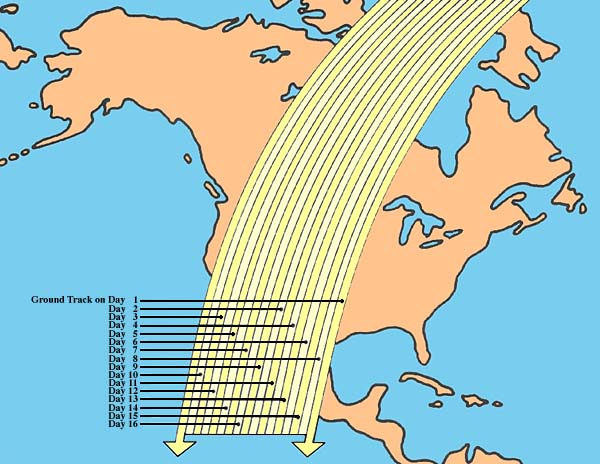
\includegraphics[width=\textwidth,height=\textheight,keepaspectratio]{figuras/swath_width_LANDSAT-NASA.jpg}
    \caption{Faixa de cobertura di�ria realizado pelo LANDSAT, ilustrado no continente Norte Americano. Para obter toda a extens�o amaz�nica � necess�rio de 16 a 26 dias, dependendo das condi��es clim�ticas do local.  }
    \FONTE{\citeonline{Nasa:swath_landsat:2015}}
    \label{fig:swath_width_LANDSAT-NASA}
\end{figure}

\subsection{Metodologia}
\label{ch:prodes_metodo}

Para realizar o c�lculo da taxa de desmatamento, as imagens s�o selecionadas de modo a obter a menor cobertura de nuvens poss�vel, melhor visibilidade com uma adequada qualidade radiom�trica\footnote{A resolu��o radiom�trica � dada pelo n�mero de n�veis de cinza, usados para expressar os dados coletados pelo sensor. Quanto maior o n�mero de valores, maior � a resolu��o radiom�trica \cite{Monteiro2008}.} e com a data de aquisi��o das imagens pr�xima ao per�odo de refer�ncia para o c�lculo da taxa de desmatamento. Por�m, considerando o hist�rico climatol�gico da Amaz�nia, a maioria das imagens n�o se apresentam livres de nuvens. Por isso � necess�rio utilizar mais de uma imagem (inclusive de outros sat�lites) para compor as cenas, formando um mosaico (Figura \ref{fig:prodes_mosaico}).

\begin{figure}[htb]
    \centering
    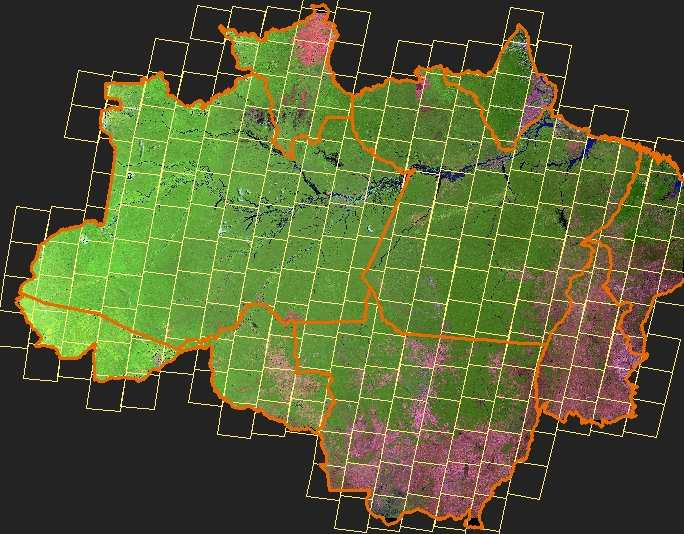
\includegraphics[width=\textwidth,height=\textheight,keepaspectratio]{figuras/mosaico_landsat-prodes.png}
    \caption{ Mosaico formado por imagens LANDSAT a serem utilizadas no sistema PRODES.}
    \FONTE{\citeonline{Monteiro2008}}
    \label{fig:prodes_mosaico}
\end{figure}

Ap�s a sele��o das imagens, a pr�xima etapa envolve transformar seus dados radiom�tricos em componentes de cena (vegeta��o, solo e sombra), utilizando o Modelo Linear de Mistura Espectral (MLME) \cite{Monteiro2008}. As bandas 3, 4 e 5 do sensor TM s�o utilizadas para estimar a propor��o dos componentes solo, vegeta��o e sombra para cada pixel, formando um sistema de equa��es lineares que pode ser solucionado pelo m�todo dos m�nimos quadrados ponderados. O resultado desse modelo linear � uma imagem fra��o, onde se tem tr�s bandas sint�ticas com os valores proporcionais de vegeta��o, solo e sombra. A segmenta��o\footnote{Segmenta��o de imagem � a subdivis�o de uma imagem em regi�es cujos \textit{p�xeis} possuam propriedades semelhantes \cite{Monteiro2008}.} da imagem fra��o � ent�o realizada, ajustando-se os limiares de similaridades e de �rea.

Um algoritmo de classifica��o n�o-supervisionado de agrupamentos de dados trata as imagens segmentadas, classificando-as de acordo com as classes definidas pelo banco de dados. Como resultado tem-se uma nova imagem \textit{raster}. Ent�o, um fotointerprete tem a tarefa de analisar os pol�gonos tem�ticos gerados, tomando a decis�o se esses devem ser aceitos ou reclassificados. Uma vez essa imagem aceita, uma m�scara de desmatamento contendo as �reas de corte raso j� detectados � gerada. Essa m�scara ser� utilizada para eliminar desmatamentos antigos, impedindo que sejam identificados novamente.

\section{DETER}
\label{ch:deter}

Devido ao tempo necess�rio para gerar os resultados e por observar apenas �reas de corte raso, o PRODES n�o pode ser utilizado como um sistema de preven��o de desmatamento. Portanto, a partir de 2004 o Sistema de Detec��o de Desmatamento em Tempo Real (DETER) foi implementado para realizar o monitoramento cont�nuo do desmatamento e da degrada��o florestal. Esse sistema foi criado para atender ao Governo Federal no Plano de A��o para a Preven��o e Controle do Desmatamento na Amaz�nia Legal. O principal objetivo desse sistema � de fornecer informa��es sobre o local e a dimens�o aproximada de ocorr�ncias de mudan�as na vegeta��o de modo a agilizar a fiscaliza��o \cite{Monteiro2008}.

\subsection{Metodologia}
\label{ch:deter_metodo}

As imagens utilizadas por esse sistema s�o obtidas pelo sensor MODIS (a bordo dos sat�lite TERRA e ACQUA da NASA), que cobre a Amaz�nia aproximadamente a cada um dia e meio (Figura \ref{fig:swath_width_MODIS-TERRA}. Essa alta resolu��o temporal reduz as limita��es de observa��o impostas pela cobertura de nuvens da regi�o. Com a m�xima resolu��o espacial limitada em aproximadamente $250$ metros, as imagens desses sensores permitem a detec��o de desmatamentos apenas para �reas maiores do que $25$ hectares. O objetivo do DETER � de fornecer indicadores para fiscaliza��o a cada 15 dias, quando as condi��es de observa��o s�o favor�veis. Esse sistema observa diversos est�gios de desmatamento para emitir seus alertas, como o de corte raso, degrada��o florestal de intensidade alta, m�dia e baixa, sendo o �ltimo mais dif�cil devido a resolu��o das imagens do sensor MODIS \cite{Monteiro2008}.

\begin{figure}[htb]
    \centering
    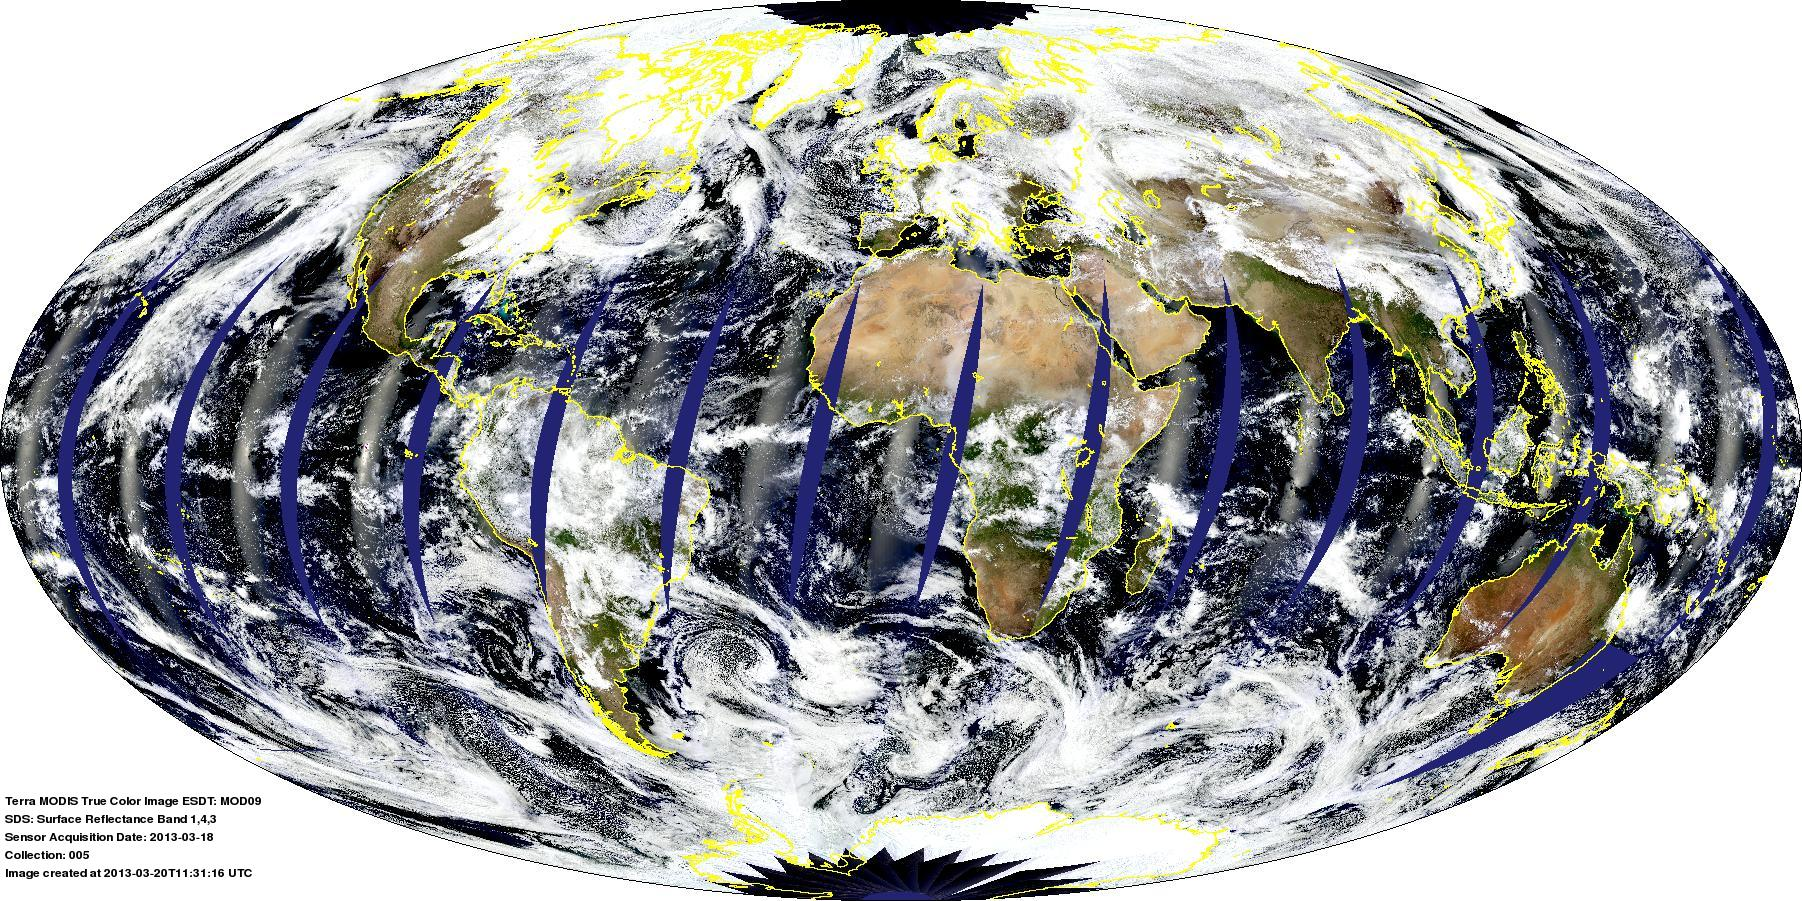
\includegraphics[width=\textwidth,height=\textheight,keepaspectratio]{figuras/swath_width_MODIS-TERRA.jpg}
    \caption{Faixa de cobertura di�ria obtida a cada sobrevoo. Para obter toda a extens�o amaz�nica � necess�rio em m�dia um dia e meio.}
    \FONTE{\citeonline{Nasa:swath:2015}}
    \label{fig:swath_width_MODIS-TERRA}
\end{figure}

A aquisi��o das imagens � feita de forma r�pida, uma vez que que o DETER utiliza os produtos baseados em \textit{granules}\footnote{Granules s�o produtos gerados de uma �rea particular. Granules n�o cobrem todo o globo.} dos subconjuntos de resposta r�pida da NASA. Esses dados encontram-se prontos\footnote{\url{https://earthdata.nasa.gov/data/near-real-time-data/rapid-response/}} para serem utilizados, pois j� foram processados, disponibilizados em GeoTIFF, RGB equivalente, no formato de 8-bits e geograficamente projetados \cite{Nasa:swath:2015,Nasa:swath_landsat:2015}.

Essas imagens s�o ent�o carregadas no Sistema de Processamento de Informa��es Georreferenciadas (SPRING) para que outros processamentos sejam feitos. Nesta etapa, o especialista necessita aplicar um modelo de mistura para separar o que � floresta, solo ou �gua (ou sombra). Essa etapa � feita selecionando-se certos \textit{p�xeis} com uma resposta espectral particular. Ent�o, cada imagem � segmentada e classificada. Ap�s a classifica��o das imagens, o especialista aplica as m�scaras dos desflorestamentos anteriores e de hidrografia, com a finalidade de esconder os desmatamentos j� conhecidos assim como outras caracter�sticas.

Na �ltima etapa, o especialista corrige os resultados da segmenta��o autom�tica, pixel a pixel. As vezes � poss�vel que as etapas de classifica��o e segmenta��o possam ser colocados de lado, pois o especialista pode extrair todas as informa��es baseando-se apenas em sua experi�ncia olhando para as imagens do sat�lite, munido dos arquivos geogr�ficos de desflorestamento pr�vio e hidrografia.

\begin{figure}[htb]
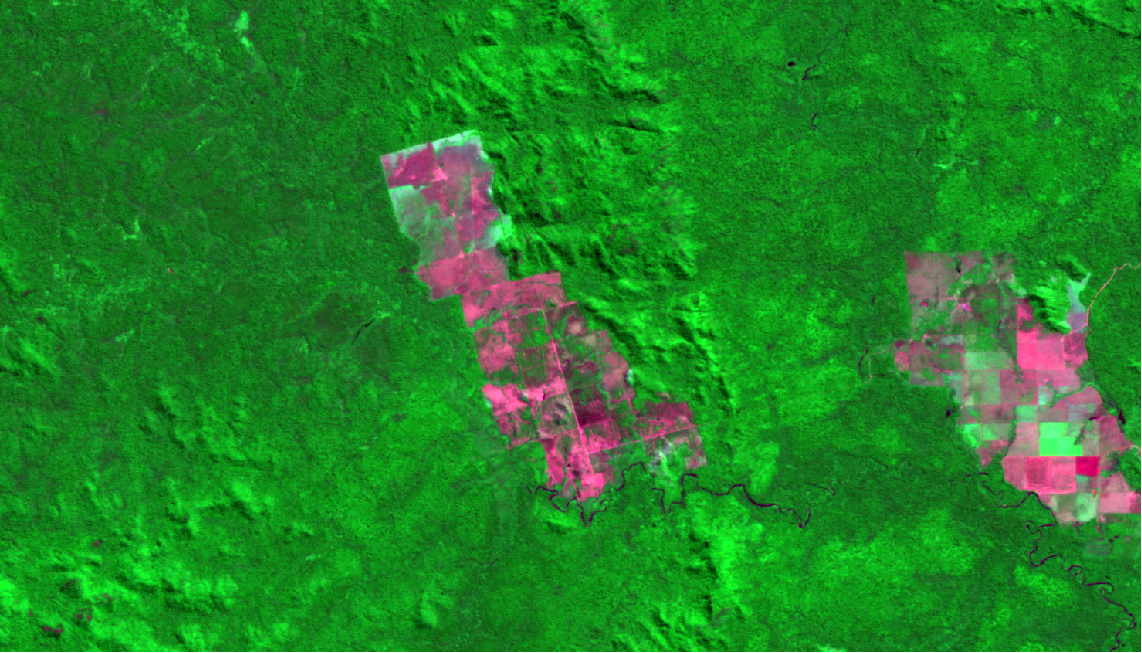
\includegraphics[width=0.485\textwidth]{figuras/COMPARE_RESOURCESAT.png}
\hfill
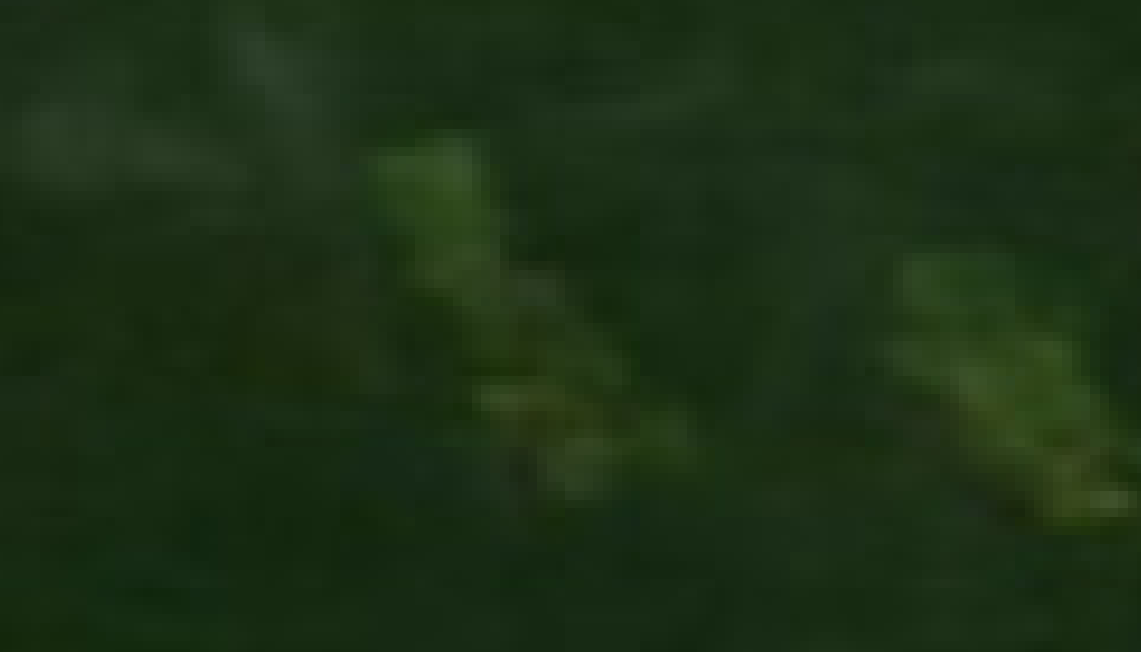
\includegraphics[width=0.485\textwidth]{figuras/COMPARE_MODIS.png}
\caption{Compara��o de diferentes resolu��es espaciais. � esquerda, uma imagem RESOURCESAT com 23,5 m por pixel. � direita, uma imagem MODIS com 250 m por pixel.}
\label{fig:comparacao_resourcesat_modis}
\end{figure}

\chapter{CI�NCIA CIDAD�}
\label{ch:ciencia_cidada}

Ci�ncia cidad� � o termo usado para designar projetos no qual volunt�rios, muitos sem nenhum treinamento cient�fico espec�fico, participem de ou gerenciem certas atividades cient�ficas, tais como a realiza��o de observa��es, medi��es ou computa��o \cite{SoaresSant:2011:EnPoAt}.

Atrav�s do voluntariado de pessoas comuns, conhecidas como cientistas cidad�os, projetos cient�ficos conseguem obter um quadro maior de colaboradores \cite{Cohn.2008}, um fator importante em projetos grandes, agilizando o processo de aquisi��o e divulga��o dos resultados. Segundo \citeonline{Silvertown2009}, o cientista cidad�o � um volunt�rio que coleta ou processa dados como parte de uma pesquisa cient�fica. Cientistas cidad�os n�o s�o respons�veis, necessariamente, por analisar ou publicar artigos cient�ficos; em geral estes desempenham tarefas simples, mas de grande import�ncia para a conclus�o dos trabalhos cient�ficos. Nas �ltimas d�cadas, projetos cient�ficos baseados em ci�ncia cidad� ganharam notoriedade, por�m esta abordagem n�o � nova para a comunidade cient�fica.

Realizar pesquisas cientificas utilizando-se da colabora��o de diversos indiv�duos n�o � novidade, antigamente diversos cientistas realizavam suas pesquisas desta forma. J� no s�culo XIX, Charles Darwin em "A Origem das Esp�cies" \citeonline{darwin-origin-of-species-1859} contou com a ajuda de mais de dois mil colaboradores e pesquisadores de diferentes �reas.  De acordo com o projeto \textit{Darwin Correspondences}\footnote{\url{http://www.darwinproject.ac.uk/}}, Darwin trocou mais de 7.500 das cartas com correspondentes durante sua pesquisa \cite{DarwinProject_Correspondents}. Os conte�dos destas cartas variavam de anota��es cient�ficas sobre algumas esp�cies, o que requeria um aparato profissional, at� simples observa��es, que vieram a colaborar com teoria da evolu��o das esp�cies.

Naquela �poca, as cartas demoravam meses para serem recebidas e lidas, o processo de responder uma carta e obter um novo retorno da mesma pessoa, chegava a levar anos para acontecer. A falta de infraestrutura e de tecnologias, tornavam a tarefa de entregar uma carta, que hoje em dia � simples e comum, um trabalho dif�cil e lento. Naquela �poca, o servi�o de correspond�ncia era feito por mensageiros a p�, a cavalo ou atrav�s de charretes, tendo navios � vela para transporte mar�timo das correspond�ncias. \citeonline{Hyde1891} relembra que para a determinada �poca, estes servi�os eram caros e n�o acess�vel para todos, o que dificultava ainda mais o compartilhamento de ideias. Em 1840, com a grande reforma de postagem brit�nica, \textit{Uniform Penny Postage}\footnote{A reforma realizada pela \textit{Royal Mail} do Reino Unido cobrava apenas um \textit{Penny}, menor moeda do sistema monet�rio da �poca, para entregar as cartas indiferente da dist�ncia \cite{BritishPostalMuseum2015,Hyde1891}.}, houve uma maior difus�o e uso dos servi�os, elevando o envio de cartas de 82.500.000 para 169.000.000 em um ano, mais que o dobro \cite{Hyde1891}.

\citeonline{Zimmer2011}, comenta que um projeto de ci�ncia cidad� como o Evolution MegaLab \cite{Silvertown2011} seria possivelmente uma das formas de Darwin fazer ci�ncia hoje. Neste projeto, mudan�as evolucion�rias s�o observadas em tempo real por diversos colaboradores, que coletam e enviam informa��es sobre as cores das cascas de duas esp�cies de caramujos, \textit{Cepaea nemoralis} e \textit{C. hortensis}.

Mais recentemente, um projeto da universidade de Oxford ir� investigar o envolvimento do p�blico na ci�ncia do s�culo XIX ao XXI. Este projeto receber� o financiamento de quase 2 milh�es de libras para realizar seus estudos \cite{conscicom2014}, e dever� ajudar a conceber e desenvolver novas ferramentas para troca de informa��es entre cientistas profissionais e legi�es de volunt�rios \cite{Leicester2013}.

\section{Ci�ncia Cidad� Moderna}
\label{ch:ciencia_cidada_moderna}

O projeto considerado um dos primeiros de ci�ncia cidad� moderno � o \textit{Christmas Bird Count}. Um projeto antigo e que ainda encontra-se em atividade, o Christmas Bird Count procura contar as diferentes esp�cies que existem na Am�rica do Norte, suas eventuais mudan�as de habitat, entre outras informa��es. O projeto foi idealizado em 1900 por Frank Chapman, um famoso ornit�logo do Museu Americano de Hist�ria Natural, como uma atividade alternativa ao evento de ca�a aos p�ssaros existente na �poca. Chapman publicou diversos livros com os resultados obtidos por este projeto com a ajuda de milhares de volunt�rios. Os volunt�rios seguem diversas regras para conduzir a pesquisa durante os 20 dias em que as observa��es s�o feitas, de 14 de dezembro a 5 de janeiro de cada ano, s� podem ser contabilizados os p�ssaros que forem avistados ou ouvidos em um di�metro de 24 km, moradores pr�ximos a estas �reas podem utilizar bebedouros para p�ssaros para atrair mais esp�cies e contabiliz�-los \cite{Silvertown2009}. Em uma contagem recente, milhares de observadores relataram mais de $63$ milh�es de p�ssaros.

Hoje, o centro de pesquisa que deu origem a este projeto � considerado um dos maiores centros especializados em ci�ncia cidad� com diversos estudos em biologia. Cientistas do laborat�rio Cornell de Ornitologia da universidade de Cornell, l�deres no estudo e conserva��o dos p�ssaros, rastreiam projetos que utilizam ci�ncia cidad� para realizar seus estudos. Estes acreditam que trabalhar com cientistas cidad�os � um fen�meno em expans�o em todo o mundo \cite{Cohn.2008}. Este laborat�rio conta com uma comunidade de aproximadamente 200 mil participantes em projetos de ci�ncia cidad�.

Ainda h� d�vidas se os projetos de ci�ncia cidad� possam gerar resultados confi�veis, uma vez que muitos dos volunt�rios engajados nas atividades cient�ficas n�o possuem conhecimento nem mesmo familiariza��o com as ferramentas de coleta. Esta � uma quest�o muito pertinente e recorrente do meio. H� evid�ncias \cite{Silvertown2009,Silvertown2011,Cohn.2008} que estes dados produzidos por cidad�os comuns s�o confi�veis. Para garantir a confian�a nestes dados � necess�rio que algumas medidas sejam seguidas.

Para alguns tipos de projetos, \citeonline{Cohn.2008} defende que os volunt�rios devam possuir algum tipo de treinamento b�sico, para que os dados sejam coletados conforme o solicitados pelos cientistas, assim diretrizes devem ser definidas. Parte dessas diretrizes deve limitar o trabalho do volunt�rio, especificando um determinado foco de coleta, por exemplo. Esta especifica��o evita diversos ru�dos nos dados e ao comparar a coleta feita entre os volunt�rios, os dados seguir�o a mesma sem�ntica, facilitando a verifica��o de erros. H� relatos que projetos anteriores baseados em ci�ncia cidad�, possu�am resultados variados por causa destes ru�dos, ao inv�s de dados exatos \cite{Cohn.2008}. Solicitar que os volunt�rios desempenhem trabalhos simples auxilia na exatid�o dos dados.

\citeonline{Silvertown2009} enumera tr�s fatores cruciais para o aparecimento de projetos de ci�ncia cidad� nos �ltimos anos. Primeiramente, a internet como meio de disseminar informa��es e adquirir dados do p�blico, assim como a tecnologia dos \textit{smartphones}, onde mais e mais aplicativos utilizam diversos sensores para coletar diferentes dados. Segundo fator se deve aos cientistas profissionais perceberem que volunt�rios s�o uma fonte sem custos de trabalho e habilidades pessoais como tamb�m de poder computacional, projetos que requerem adquirir diversos dados ao longo do globo, necessitam de ajuda, podendo ser de volunt�rios, para se obter sucesso. Terceiro fator, financiadores de projetos cient�ficos procuram beneficiar projetos que utilizam cientistas cidad�os em seus trabalhos.

Com o aparecimento destes novos projetos, a ci�ncia cidad� moderna pode ser classificadas em tr�s formas, conforme o n�vel de envolvimento do volunt�rio e a tecnologia utilizada no projeto (Figura \ref{fig:pt_citizen_science}).

\begin{figure}[htb]
    \centering
    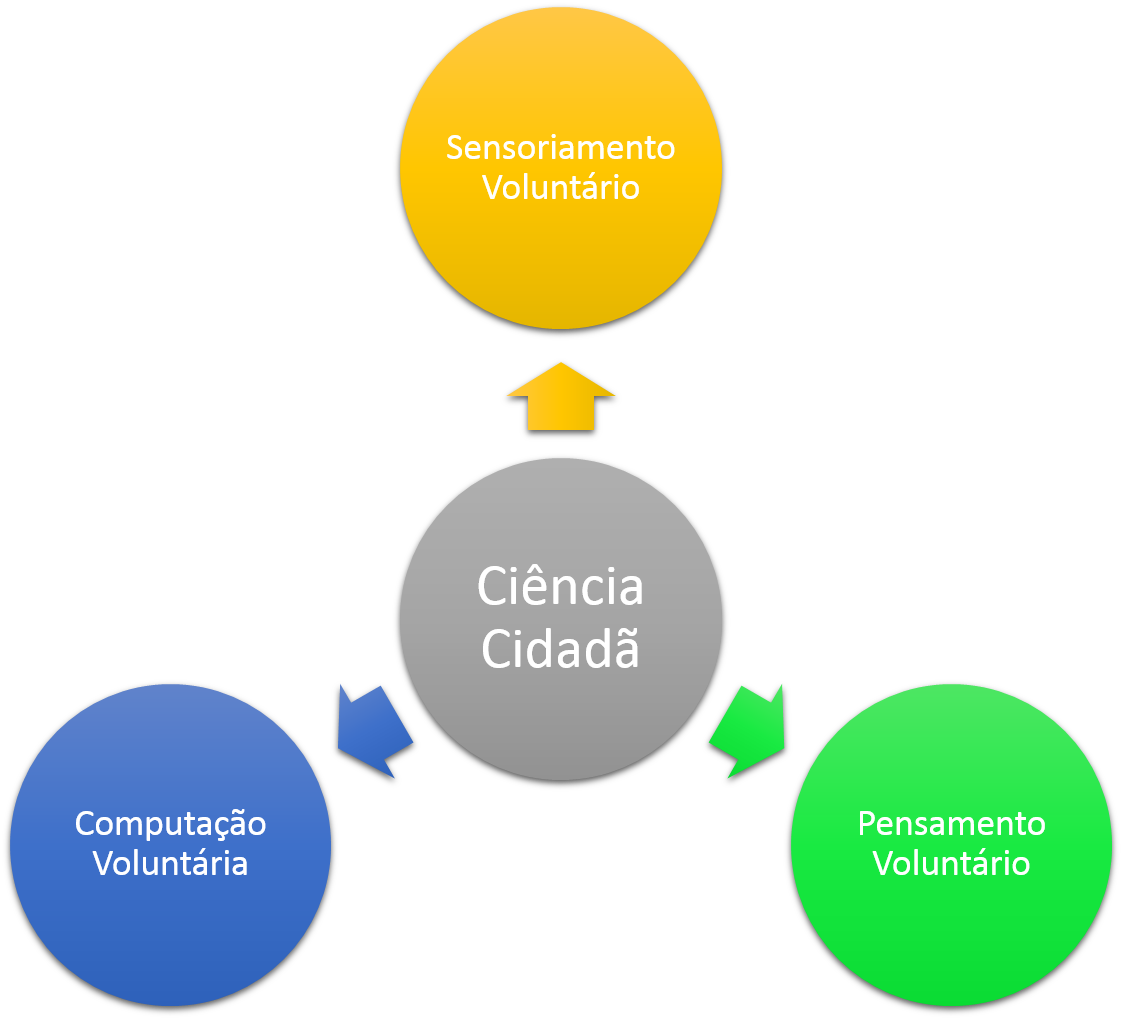
\includegraphics[width=\textwidth,height=\textheight,keepaspectratio]{figuras/pt_citizen_science.png}
    \caption{A ci�ncia cidad� pode ser classificadas em tr�s formas: computa��o volunt�ria, onde os volunt�rios doam o poder computacional de suas m�quinas para pesquisas cient�ficas; pensamento volunt�rio utilizado em projetos que requerem a cogni��o dos volunt�rios, como classifica��o de imagens; e sensoriamento volunt�rio onde a capta��o de dados � crucial para a pesquisa.}
    \label{fig:pt_citizen_science}
\end{figure}

Estas formas ser�o introduzidas a seguir.

\section{Computa��o Volunt�ria}
\label{ch:computacao_voluntaria}

Recentemente, o n�mero de projetos que se beneficiam de ci�ncia cidad� est� aumentando, cada dia h� novos projetos surgindo. Estes projetos chamados de ci�ncia cidad� moderno est�o se tornando frequente por causa da acessibilidade das tecnologias atuais, o que n�o requer aparatos especializados para realizar as pesquisas. Como mencionado anteriormente, as informa��es que \citeonline{Darwin1859} utilizou em suas pesquisas foram enviadas atrav�s de cartas que demoravam muitos meses para chegar a seu destinat�rio. Hoje, com o avan�o da internet, volunt�rios em diferentes partes do mundo podem fornecer diferentes tipos de dados a uma pesquisa. Seja por dispositivos m�veis, que uma vez ligados a internet podem fornecer dados de qualquer lugar, ou ent�o por meio de computadores.

Na d�cada de 80, a internet ainda era apenas um embri�o e poucos tinham acesso � rede. Existiam menos de 200.000 servidores espalhados no mundo. At� ent�o n�o existiam p�ginas para serem navegadas, a principal forma de troca de mensagem era atrav�s de e-mail, criado em 1977 \cite{HistoryOfInternet:David,HistoryOfInternet:Anthony}, outros meios eram por TELNET e IRC, apenas. S� no in�cio da d�cada de 90 que as primeiras p�ginas de internet foram criadas, ap�s a defini��o do \textit{WWW}\footnote{World Wide Web} criado por \citeonline{berners1992world}. A internet estava tornando-se popular, com seus aproximados 1 milh�o de servidores e suas 50 p�ginas de internet \cite{HistoryOfInternet:Anthony}.

Com a populariza��o da internet, iniciou-se a apari��o de projetos not�veis da ci�ncia cidad� moderna. Os computadores da �poca eram caros e possu�am pouco poder computacional, apenas grandes ind�strias e universidades tinham acesso a m�quinas de grande desempenho. Neste per�odo, surgiram os primeiros projetos de computa��o volunt�ria, onde os volunt�rios doavam o tempo de processamento ocioso de suas m�quinas a projetos que necessitavam de grande poder computacional para trabalhar em cima dos seus dados. O conceito desta forma de projeto era de dividir a grande massa de dados existente em pequenas por��es que fossem poss�veis para os volunt�rios efetuar downloads, visto que naquela �poca n�o havia internet de banda larga. A forma de conex�o � internet ainda era discada e o modem mais r�pido deste per�odo era o de 56 Kbps\footnote{56 \textit{kilobits} por segundo} \cite{AndersonCKLW02}.

No meio da d�cada de 90, surgiram os projetos \textbf{\textit{GIMPS}}\footnote{\textit{\url{http://www.mersenne.org/}-Great Internet Mersenne Prime Search}} e \textbf{\textit{Distributed.net}}\footnote{http://www.distributed.net/}\cite{Anderson1999,AndersonCKLW02,Hayes1998}.

\textit{GIMPS} foi o primeiro projeto de computa��o volunt�ria de grande porte a ser realizado, \textit{GIMPS}, tinha como objetivo encontrar n�meros primos de Mersenne, nome dado em homenagem ao estudioso Marin Mersenne da teoria dos n�meros. A formula destes n�meros equivale  $ M_n = 2^n -1 $, onde $n$ � um n�mero natural. O desafio de descobrir n�meros de Mersenne est� diretamente ligado ao fato destes n�meros serem exponenciais, tendo assim milhares de d�gitos em sua composi��o. At� 1996, in�cio do projeto \textit{GIMPS}, apenas 34 n�meros primos de Mersenne eram conhecidos, logo no primeiro ano do projeto foram descobertos mais dois  n�meros, $ M_{1398269} $ e $M_{2976221}$. O primeiro n�mero possui $852.365$ algoritmos, o segundo $1.814.262$, uma opera��o que seria imposs�vel para ser realizada por uma pessoa. Ambos foram descobertos na primeira vers�o do software disponibilizado pelo projeto, sendo calculado por um computador \textit{Pentium} 90 MHz e \textit{Pentium} 100MHz, respectivamente. Hoje, h� o conhecimento de 48 n�meros de Mersenne, sendo o �ltimo n�mero descoberto o $M_{57885161}$ com $17.425.170$ d�gitos em 2013, desde o in�cio do projeto foram descobertos 14 destes n�meros \cite{Marsenne:Primes,Hayes1998}.

A \textit{Distributed.net}, lan�ado em 1997, tinha o principal objetivo de quebrar a criptografia gerada pela empresa RSA, para o desafio \textit{RSA Secret-Key Challenge} que correspondia a uma chave de 56-bit e possu�a uma recompensa de $10.000,00$ d�lares. O projeto criado por Earle Ady e Christopher G. Stach II, contava com a colabora��o de mais de $300.000$ volunt�rios utilizando o tempo de seus computadores realizando um ataque de For�a Bruta\footnote{For�a Bruta � a forma de tentar obter a a resposta de uma senha atrav�s de in�meras tentativas.} em cima de parte do c�digo disponibilizado para o desafio. Em 250 dias a chave foi descoberta, utilizando um poder computacional equivalente a 26 mil \textit{Pentium} 200 MHz. Outro desafio com uma chave de 64-bit tamb�m foi conclu�do ap�s 4 anos e o pr�mio pago. A empresa de seguran�a RSA, havia dito que para quebrar uma chave de 64-bit, seria necess�rio mais de 100 anos testando todas as possibilidades e combina��es. Atualmente o projeto est� focado em quebrar uma chave de 72-bit \cite{distributed.net:online,Distributed.net:wired}.

Em 1999, \citeonline{AndersonCKLW02} iniciou um dos primeiros e mais bem sucedido projeto de ci�ncia cidad�. O objetivo deste projeto era de encontrar vida inteligente no espa�o, atrav�s da an�lise de sinais de r�dios captadas do espa�o, \textit{SETI@Home}. Por�m para conseguir analisar esses sinais, o projeto contou com o uso de diferentes computadores, espalhados pela internet formando um grande sistema distribu�do de processamento. Os volunt�rios que se cadastravam no s�tio podiam fazer download de um aplicativo que s� era ativado quado o computador estava em modo ocioso. O aplicativo recebia pacotes de sinais a serem analisados e no fim do processamento enviava os resultados obtidos ao servidor do projeto.

\section{Pensamento Volunt�rio}
\label{ch:pensamnto_voluntario}
\citeonline{Anderson1999}, a frente do projeto \textit{SETI@Home}, iniciou o desenvolvimento de uma nova plataforma computacional para diminuir as barreiras que ele havia encontrado ao longo do desenvolvimento do seu �ltimo projeto, viabilizando assim novas iniciativas para utilizar computa��o volunt�ria de forma r�pida e sem grandes conhecimentos de computa��o. Chamada de BOINC\footnote{Berkeley Open Infrastructure for Network Computing}, seu objetivo era de avaliar a exatid�o e veracidade dos dados antes de envi�-los aos servidores dos projetos \cite{anderson2003public}. Esta ferramenta j� foi utilizada por mais de 150 projetos, tendo atualmente 70 projetos online. Estes fatos s� foram alcan�ados pela acessibilidade que novos projetos do tipo de computa��o volunt�ria tiveram com a cria��o da nova ferramenta e tamb�m pela visibilidade que a ferramenta deu aos projetos deste porte.

Al�m da ferramenta \textit{BOINC} realizar verifica��es redundantes para melhorar a exatid�o dos resultados, esta tamb�m classificava os usu�rios e mantinha um hist�rico da pontua��o de cada usu�rio conforme seu comprometimento em rela��o aos projetos. Na p�gina da ferramenta, existem diversas estat�sticas dos projetos em andamento, estas estat�sticas s�o atualizadas dinamicamente conforme os resultados s�o submetidos pelos volunt�rios. Uma vez que os novos resultados s�o submetidos e aprovados, cada volunt�rio tem o valor da sua contribui��o ao projeto calculado novamente. Tendo assim um sistema de cr�ditos, que pontua a participa��o dos volunt�rios, destacando os que mais contribuem. Este � considerado o sistema de recompensa dos usu�rios, levando o projeto a ter cada vez mais volunt�rios contribuindo com a performance da sua m�quina para ganhar notoriedade \cite{Anderson1999}.

No fim da d�cada de 90, \citeonline{dinucci1999fragmented} cunhou o termo \textit{Web 2.0} dizendo que a internet at� ent�o n�o tinha mostrado o seu real potencial. As p�ginas eram simplesmente recursos est�ticos onde a navega��o era composta de uma simples requisi��o a este recurso e o recurso era ent�o exibido na tela dos computadores da �poca. A revolu��o da \textit{Web 2.0} seria marcada pela interatividade do conte�do, permitindo a qualquer pessoa utilizando um computador ou dispositivo m�vel, n�o mais carregar um simples recurso est�tico, mas sim o poder de interagir com este recurso, expressando ideias e adicionando novas informa��es a \textit{Web}. Diversas novas ferramentas foram criadas nesta nova era. Diferentes tipos de \textit{blogs}, \textit{wikis} e p�ginas de internet repletos de conte�dos din�micos.

Com a possibilidade de conte�do din�mico e a intera��o dos usu�rios, surgiram novos tipos de projetos que passaram a utilizar a capacidade cognitiva dos volunt�rios para analisar visualmente determinados dados e em fun��o destes tomar a��es.

Um dos primeiros projetos de pensamento volunt�rio foi criado para detectar pequenas part�culas de poeira interestelar coletada pela miss�o \textit{Stardust} da NASA, lan�ada em 1999 \cite{Stardust:Mission}. Andrew Westpahl, o idealizador do projeto \textit{Stardust@Home} teve a ideia de utilizar a cogni��o dos usu�rios para substituir a falta de uma tecnologia de reconhecimento de padr�o capaz de encontrar as part�culas min�sculas coletada pela miss�o. Westpahl estimou que levaria mais de um s�culo para sua equipe poder atingir o objetivo do projeto sem a ajuda dos volunt�rios. Para encontrar as part�culas, foi disponibilizado no in�cio do projeto em 2006, 1,6 milh�es de imagens na p�gina do projeto. Estas imagens recriam a experi�ncia que um cientista teria se estivesse analisando as amostras atr�s de part�culas atrav�s de um microsc�pio, estabelecendo uma melhor imagem pelo ajuste do seu foco. Estas 1,6 milh�es de imagens foram feitas para simular esta fun��o e s�o chamadas de ``filmes de foco''. Assim diversas imagens foram feitas de um determinado ponto mas utilizando posi��es diferentes para se ter uma melhor nitidez da imagem. � fun��o do volunt�rio verificar se esta imagem est� bem focada, verificando a nitidez das imagens disponibilizadas e se h� alguma part�cula presente em alguma destas imagens\cite{Hand2010}. Caso n�o exista nenhuma imagem focada, o volunt�rio deve informar atrav�s do s�tio esta situa��o, assim como outras diversas situa��es que podem acontecer. Para conhecer essas determinadas situa��es, os volunt�rios necessitam realizar um treinamento antes de iniciar o seu trabalho de volunt�rio efetivamente, neste treinamento h� dicas e orienta��es de como proceder. Este tipo de treinamento de qualifica��o � muito comum em projetos de ci�ncia cidad� \cite{Silvertown2009,Anderson1999}.

Apesar do projeto \textit{Stardust@Home} possuir o sufixo \textit{@Home}, este n�o utiliza a ferramenta BOINC, idealizada por \citeonline{anderson2003public}. Este sufixo � apenas uma homenagem aos projetos de ci�ncia cidad�. Contudo, \citeonline{Anderson1999} estudou o projeto e idealizou uma nova ferramenta para tornar projetos de pensamento volunt�rio mais comuns, assim como o uso da ferramenta BOINC. O resultado desta pesquisa foi a plataforma BOSSA\footnote{\url{http://boinc.berkeley.edu/trac/wiki/BossaIntro}}. Trata-se de um \textit{middleware} respons�vel por dividir o trabalho em tarefas menores e atribu�-las aos volunt�rios, realizando verifica��es do n�vel de assertividade das respostas dadas pelos volunt�rios atrav�s de redund�ncia das tarefas.

Em 2007, iniciou-se o projeto \textit{GalaxyZoo} com o objetivo de classificar imagens de gal�xias. As imagens captadas por um telesc�pio rob�tico, \textit{Sloan Digital Sky Survey}\footnote{http://www.sdss.org/} era apresentadas para os volunt�rios e estes tinham que decidir se a imagem continha alguma gal�xia e, se afirmativo, qual era a sua forma (el�ptica ou espiral). Se fosse espiral, ainda havia uma �ltima pergunta, qual o sentido da sua rota��o\cite{Hand2010}. Pelo n�mero de imagens que deveriam ser classificadas, os cientistas envolvidos acreditavam que iria demorar mais de 2 anos para que todas as imagens fossem classificadas\cite{GalaxyZooAbout}. Por�m, com apenas um dia de funcionamento, o \textit{GalaxyZoo} conseguiu reunir 35 mil volunt�rios que fizeram aproximadamente 1.5 milh�es de classifica��es. O projeto classificou perto de um milh�o de gal�xias utilizando-se de mais de 150 mil volunt�rios. Em sua segunda vers�o, o GalaxyZoo contou com mais de 200 mil volunt�rios para classificar de forma mais detalhada 300 mil gal�xias previamente classificadas \cite{willett2013galaxy}.

\textit{Rosseta@Home} � outro importante projeto de ci�ncia cidad�. Quando criado em 2005, este projeto seguia a mesma tend�ncia do \textit{Seti@Home} assim como os demais projetos da fam�lia \textit{@Home}, ser baseado em computa��o volunt�ria. O objetivo deste projeto � de utilizar o grande poder computacional reunido para prever o enovelamento de prote�nas, um processo qu�mico em que a estrutura de uma prote�na assume a sua configura��o funcional, podendo assim desenvolver novas prote�nas para combater diversas doen�as. Como os demais projetos da fam�lia, os volunt�rios tinham que executar o instalador do projeto utilizando o BOINC e este s� iria entrar em funcionamento quando o computador estivesse ocioso, em modo de protetor de tela. Por�m, diversos e-mails foram enviados ao projeto de volunt�rios que queriam contribuir mais, dizendo ser poss�vel obter melhores resultados se eles pudessem interagir com o modelo de prote�na que estava aparecendo ali no protetor de tela.

Com isto em mente, David Baker desenvolveu um novo projeto de pensamento volunt�rio com caracter�sticas de um jogo atrav�s da internet, onde os volunt�rios s�o os jogadores e precis�o achar as melhores solu��es para os desafios, utilizando o enovelamento de prote�nas \cite{Hand2010}. \textit{Foldit}, lan�ado em 2008, provou que os volunt�rios conseguem realizar um melhor trabalho do que um computador. Este foi um dos primeiros trabalhos a envolver tanto computa��o volunt�ria quanto o pensamento volunt�rio \cite{Cooper2010}.

Um dos resultados mais significativos, foi alcan�ado pelos jogadores do projeto \textit{Foldit} em 2011, onde os volunt�rios resolveram um problema proposto pelos pesquisadores em apenas 3 semanas. Os cientistas lan�aram o desafio a partir do instante em que os m�todos autom�ticos come�aram a n�o retornar bons resultados. Ao analisar os resultados dos jogadores, observaram que estes eram suficientemente bons para encontrar uma r�pida solu��o \cite{Khatib2011}.

\citeonline{mcgonigal2011reality} sugere que os problemas atuais poderiam ser solucionados efetivamente de outra forma, atrav�s dos jogos. Conscientizando pessoas dos problemas reais e inserindo os diversos problemas no contexto de jogos, os jogadores iriam buscar solu��es para estes desafios. Diversos pesquisadores sugerem que construir projetos de ci�ncia com a tem�tica na forma de jogos poderiam atrair ainda mais os volunt�rios e resolver ainda mais r�pido os desafios empregados \cite{Silvertown2009,Hand2010,Khatib2011,Anderson1999,Pereira:2013:NoInUs,Cooper2010,Mansell2012}.

\section{Sensoriamento Volunt�rio}
\label{ch:sensoriamento_voluntario}

As duas formas de ci�ncia cidad� discutidas anteriormente t�m suas vantagens conforme a necessidade do m�todo de pesquisa cient�fica que ir� ser executada. Computa��o volunt�ria tem maior vantagem para as atividades cient�ficas que requerem grande poder computacional, avaliando grandes quantidades de dados, o que levariam horas para uma pessoa realizar. J� o pensamento volunt�rio, mostra-se mais eficaz em atividades que requerem o poder cognitivo dos volunt�rios, como detec��es de padr�es utilizando inspe��o visual.

Algumas vezes, os dados dispon�veis para projetos cient�ficos n�o s�o suficientes e a coleta de outros tipos de medidas se faz necess�ria. Adquirir novas fontes de dados n�o � um trabalho simples pois necessita equipes capazes de efetuar as coletas cient�ficas conforme padr�es exigidos e ferramentas adequadas para tal.
Assim, a realiza��o desta tarefa, se feita apenas pelos cientistas envolvidos diretamente com o projeto, pode se tornar custosa e demorada. Portanto, uma alternativa vi�vel � a utiliza��o de sensoriamento volunt�rio onde volunt�rios contribuem com dados, sejam anota��es de observa��es, capta��o de imagem ou sons de um ambiente. A tecnologia atual permite solu��es de menor custo para coletar diversos tipos de dados para serem utilizados em projetos cient�ficos.

O sensoriamento volunt�rio � uma jun��o de Informa��o Geogr�fica Voluntariada (IGV), termo cunhado \citeonline{Goodchild2007} e usado para descrever as tarefas realizadas por volunt�rios ao fornecer dados complementares a determinadas localiza��es geogr�ficas com a finalidade de enriquecer a base de dados, com sensoriamento m�vel \cite{Lane2010}, onde pesquisas s�o conduzidas atrav�s de aparelhos m�veis dos volunt�rios utilizando os sensores do dispositivo.

\subsection{Informa��o Geogr�fica Voluntariada}
\label{ch:informacao_geografica_voluntariada}

\citeonline{Goodchild2007} categoriza de \textbf{Informa��o Geogr�fica Voluntariada (IGV)} o fen�meno que vem atraindo cidad�os de toda parte, a cria��o de informa��es geogr�ficas. Tarefa que antigamente era de uso exclusivo das ag�ncias oficiais respons�veis por realizar cartografias dos pa�ses, por�m com o avan�o da tecnologia, qualquer pessoa pode ter acesso a ferramentas de edi��o de mapa online e colaborar com alguma informa��o geogr�fica. Seja esta espec�fica sobre um determinado pr�dio, dado sua latitude e longitude, como tamb�m por vastos terrenos, ao descrever uma cidade. Este recente paradigma representa uma dram�tica inova��o e certamente ter� grandes impactos aos sistemas de informa��o geogr�fica.

Este conceito de cria��o de dados geogr�ficos por volunt�rios vem sendo amplamente estudado por diferentes frentes. Para a ind�stria, o desenvolvimento de plataformas baseado em web onde os usu�rios possam enviar seus dados. Para o governo, o conceito � estudado para poss�veis aplica��o em sistemas de alerta em caso de surtos de doen�as e o constante monitoramento dos impactos ambientais. Para pesquisadores acad�micos em como adaptar ambientes de sistemas de informa��o geogr�ficos para utilizar, armazenar e analisar os dados coletados por volunt�rios \cite{elwood2008volunteered}.

Um marcante projeto de informa��o geogr�fica voluntariada, \textit{Wikimapia}, � refer�ncia nesta categoria, onde volunt�rios podem contribuir com novas informa��es geogr�ficas simplesmente escolhendo um local (atrav�s de uma coordenada geogr�fica) e complementando a informa��o local \cite{Wikimapia:online}. Este projeto possui um objetivo ambicioso de descrever todo o globo terrestre com o m�ximo de informa��es geogr�ficas �teis reunidas atrav�s do uso de volunt�rios, organiz�-las e disponibiliz�-las para diversos outros usos p�blicos das informa��o. Atrav�s de uma interface simples, Figura \ref{fig:wikimapia}, para que os volunt�rios que n�o possuam experi�ncias com edi��o de mapas possam tamb�m, de forma r�pida e intuitiva, colaborar com o projeto. Foi lan�ado em maio de 2006 como uma ferramenta similar a Wikip�dia, onde todos podem editar seu conte�do, e em pouco tempo diversos volunt�rios j� haviam se cadastrado, com menos de 3 meses o projeto possu�a 1 milh�o de novos registros geogr�ficos criados apenas por volunt�rios. Em julho de 2012 o projeto j� atingia a marca de 19 milh�es de registros geogr�ficos criados \cite{Wikimapia:history}.

\begin{figure}[htb]
    \centering
    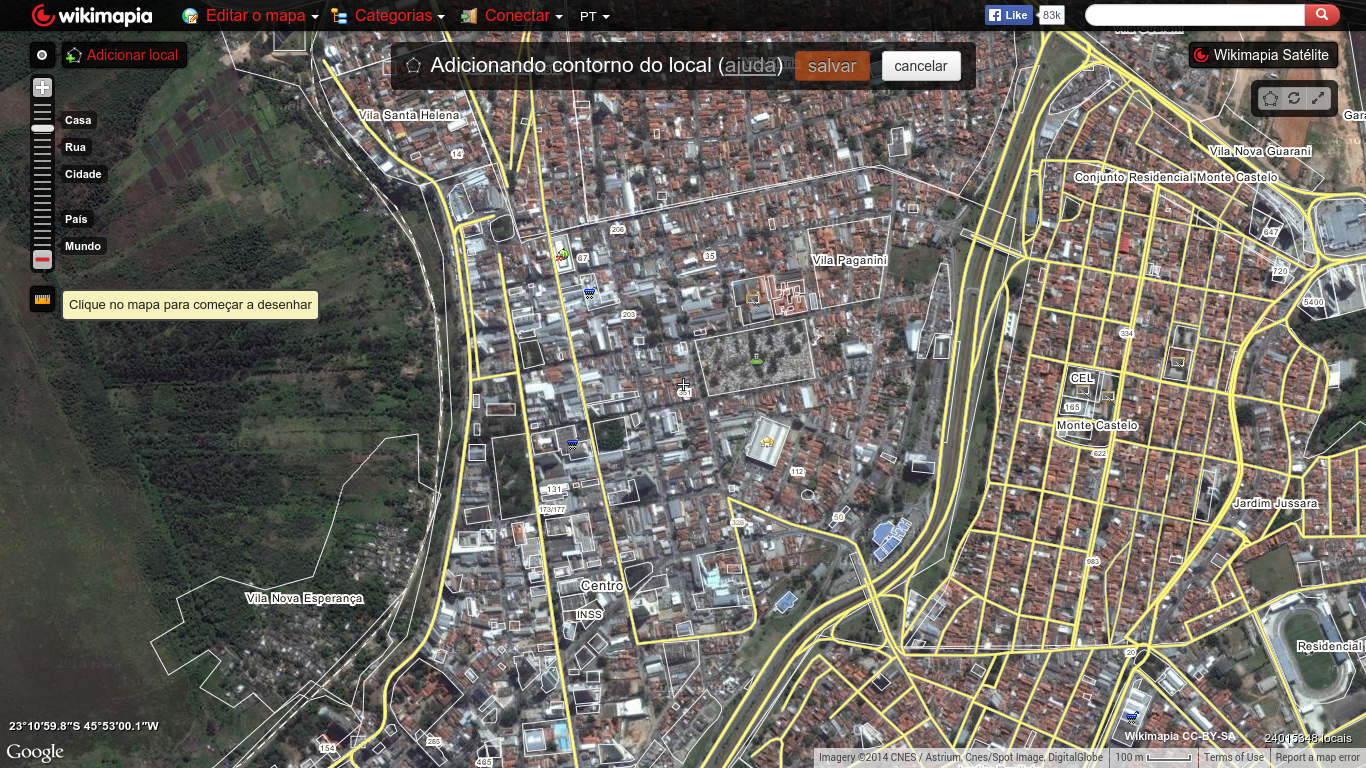
\includegraphics[width=\textwidth,height=\textheight,keepaspectratio]{figuras/wikimapia.png}
    \caption{Modo de inser��o de dados do portal \textit{wikimapia}.}
    \label{fig:wikimapia}
\end{figure}

Outro projeto que merece destaque nesta categoria � o renomado \textit{OpenStreetMaps} (OSM). Muito parecido com a ferramenta de mapas do Google, mas de forma livre, o OSM possui diferentes caracter�sticas e funcionalidades. Lan�ado em julho de 2004 e deste ent�o vem atraindo novos volunt�rios a cada dia, tendo um crescimento constante (Figura \ref{fig:osm_table}). Constru�do para que volunt�rios mantenham sempre os dados geogr�ficos atualizados, assim como o \textit{wikimapia}, por�m o OSM conta diversas funcionalidades para integra��o dos seus dados a projetos de terceiros, utilizando-se de protocolos abertos e com muitas op��es para exportar os dados.

\begin{figure}[htb]
    \centering
    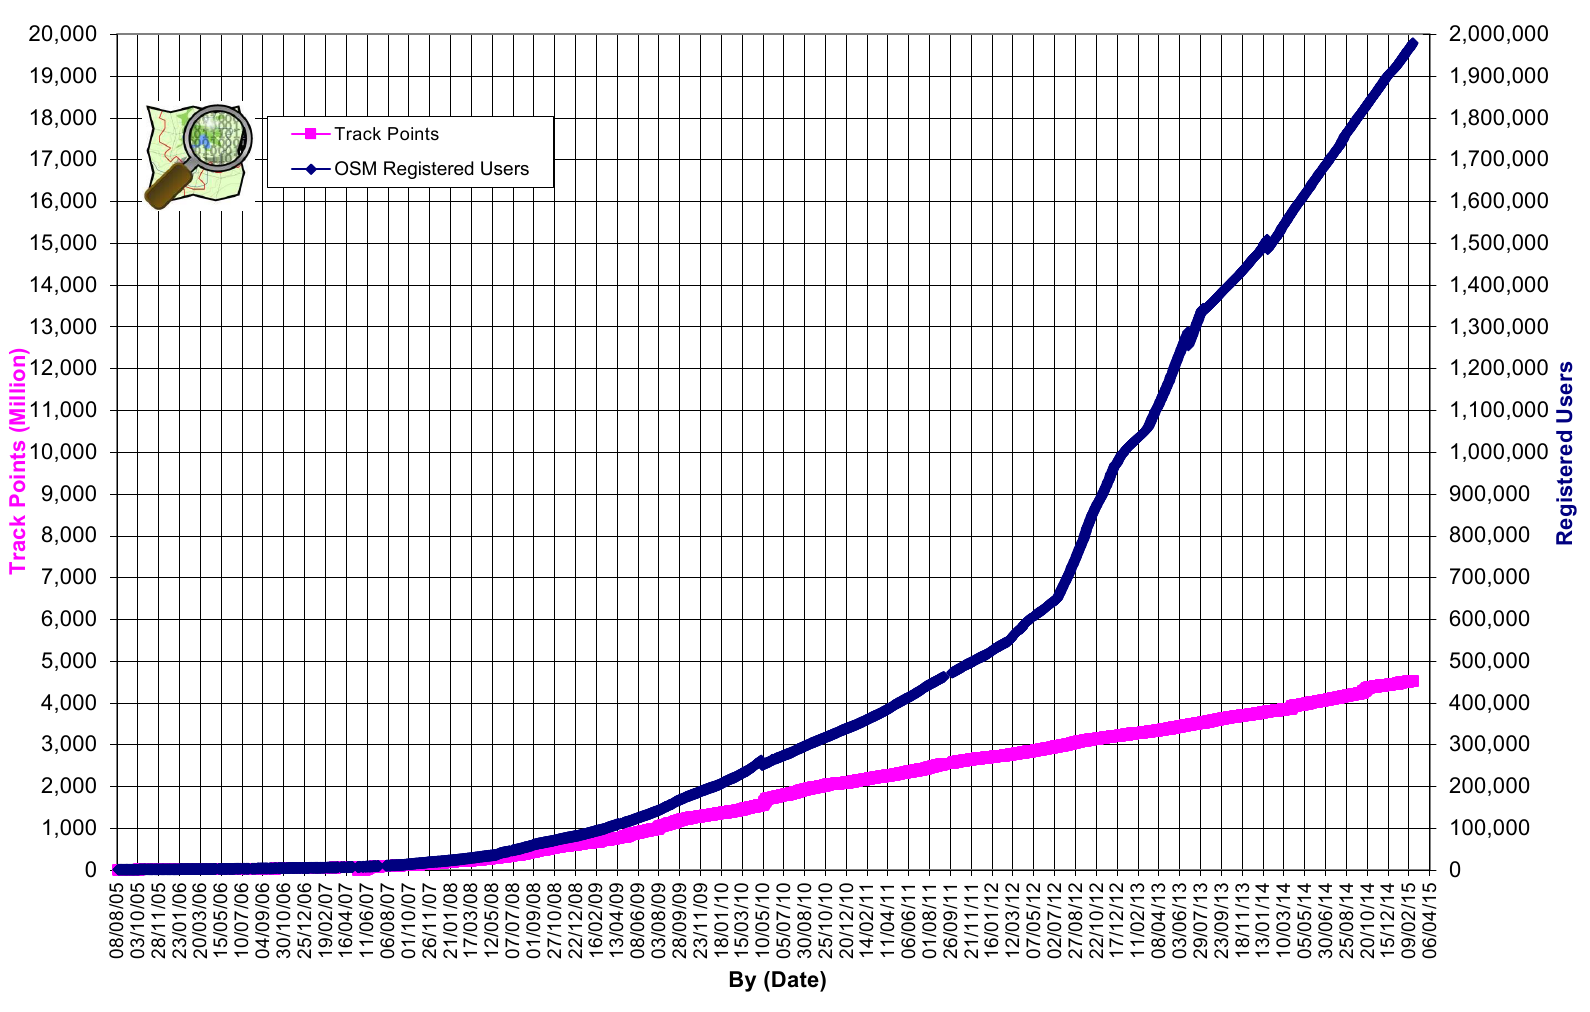
\includegraphics[width=\textwidth,height=\textheight,keepaspectratio]{figuras/osm_table3.PNG}
    \caption{Gr�fico do crescimento mensal de usu�rios registrados e contribui��es realizadas ao projeto \textit{OpenStreetMap}.}
    \FONTE{\citeonline{haklay2008openstreetmap}}
    \label{fig:osm_table}
\end{figure}

\subsubsection{Sistemas de Alertas}

Estudos sugerem que este novo conceito de explorar e criar informa��es geogr�ficas pode levar a um novo paradigma de cria��o de sistemas de alertas. Considerando cada pessoa como um sensor, h� cerca de 7 bilh�es de sensores no globo \cite{elwood2008volunteered,Goodchild2007,Gouveia2004,Gouveia2008}. Geralmente, no segundo momento ap�s um desastre como os ocasionados por furac�es e tsunamis, � dif�cil de se ter informa��es sobre os locais que foram afetados. In�meras s�o as raz�es, seja por falta de eletricidade, um bom campo de vis�o para se obter imagens de sat�lite ou aus�ncia equipamentos de comunica��o operacionais. Por�m a popula��o das �reas afetadas conhece suficientemente bem o local afetado e poderia reportar ou auxiliar atividades como de resgate, atrav�s de dispositivos m�veis via mensagens, imagens e voz. Em seu trabalho \citeonline{Schade2011} conclui que dados geogr�ficos obtidos por volunt�rios podem ser complementares aos dados de sensoriamento remoto.

\subsection{Sensoriamento M�vel}
Na era p�s-PC, mencionada pela primeira vez por \citeonline{DavidClark2013:bio}, onde os computadores deixaram de ser o principal dispositivo eletr�nico, est� se tornando realidade. Os computadores pessoais est�o sendo substitu�dos ou utilizados em outras fun��es, como h� d�cadas muitos j� previam. Sua utilidade est� mais fadada a de ser um \textit{hub} tecnol�gico, servindo de meio de comunica��o com outros dispositivos m�veis como \textit{smartphones} e \textit{tablets}. No in�cio dos anos 90, os celulares eram realidades para poucos, mas diversos fatores influenciaram a sua populariza��o ao longo do tempo. O avan�o da tecnologia permitiu, por exemplo, reduzir o tamanho dos componentes eletr�nicos e sensores f�sicos digitais, tamb�m a quantidade de energia requerida por esses.

Diversos tipos de sensores est�o cada vez mais presentes em celulares, tornando dispositivos m�veis em unidades de coleta de informa��o de grande precis�o. C�meras e sensores de localiza��o j� s�o frequentes na maioria dos celulares, permitindo obter a sua localiza��o em qualquer parte do globo terrestre atrav�s de \textit{GPS}\footnote{\textbf{G}lobal \textbf{P}ositioning \textbf{S}ystem � um sistema de navega��o baseado em uma constela��o de 24 sat�lites.}, sendo alguns modernos integrado com \textit{GLONASS}\footnote{\textbf{GLO}bal \textbf{NA}vigatsionnaya \textbf{S}putnikovaya \textbf{S}istema, um sistema de navega��o russo, constitu�do por uma constela��o de 21 sat�lites}. H� tamb�m dispositivos que apresentam sensores de proximidade, girosc�pio, magnet�metro, aceler�metro, bar�metro e sensor de luz ambiente. Al�m desses dispositivos, h� o microfone que, em conjunto com os demais sensores supracitados, pode ser utilizado como ferramenta de monitoramento ambiental.

Em recentes relat�rios, \citeonline{Gartner2014} aponta que em algum momento de 2015 os dispositivos m�veis (\textit{tablets}, celulares e \textit{smartphones}) ir�o ultrapassar os computadores pessoais (computadores de mesa e port�teis), em quantidade, conforme Figura \ref{fig:gartner}.

\begin{figure}[htb]
    \centering
    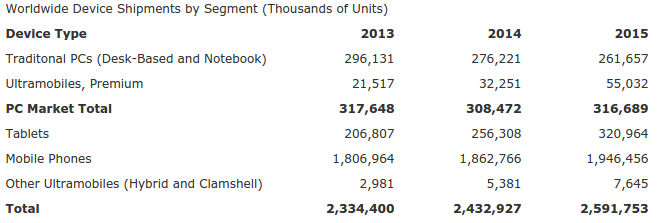
\includegraphics[width=\textwidth,height=\textheight,keepaspectratio]{figuras/gartner2014.png}
    \caption{O relat�rio Gartner de julho/2014 aponta que em 2015, o n�mero de equipamentos do tipo \textit{Tablet} ser� superior ao total do mercado do computador pessoal (computadores de mesa e \textit{notebooks}).}
    \FONTE{\citeonline{Gartner2014}}
    \label{fig:gartner}
\end{figure}

Com esta vis�o, novos projetos tem surgido com a inten��o de utilizar os sensores presentes nos dispositivos m�veis como fonte de dados cient�ficos, coletando constantemente informa��es do dia a dia de quem os utilizam \cite{Lane2010,Burke2006}.

Por anos a comunidade acad�mica e industrial vem debatendo o uso de dispositivos m�veis em pesquisas de sensoriamento, por�m sem grandes avan�os at� datas recentes. \citeonline{Lane2010} atribui esta mudan�as aos seguintes fatores:

\begin{enumerate}
    \item Sensores embarcados - utilizados primeiramente como forma de melhorar a experi�ncia de uso para os usu�rios, como aceler�metros, encontraram novas formas de uso e chamaram a aten��o de pesquisadores. Diversos sensores novos est�o revolucionando as pesquisas, como GPS e bar�metro.
    \item Programabilidade - H� uma cole��o infinita de documenta��o na internet de como programar para dispositivos m�veis de terceiros. As grandes plataformas de dispositivo m�veis, como iOS (Apple), Android (Google), e Windows Phone (Microsoft) possuem documenta��es detalhadas, permitindo qualquer pessoa com um pouco de conhecimento de programa��o aprender a linguagem e desenvolver aplicativos.
    \item Lojas de aplicativo - Os desenvolvedores de aplicativos utilizam o servi�o de loja de aplicativo do fabricante correspondente para publicar sua nova cria��o. Permitindo alcan�ar diferentes tipos de usu�rios em toda a parte.
    \item Computa��o na nuvem - Utilizando-se de computa��o na nuvem, os dispositivos m�veis podem armazenar dados e at� efetuar c�lculos atrav�s de servidores na internet, sem a necessidade de utilizar estas funcionalidades apenas local, proporcionando um grande crescimento de uso e descentraliza��o de dados.
\end{enumerate}

\chapter{FORESTWATCHERS}
\label{ch:forestwatchers}
Em uma carta enviada a revista Nature\footnote{\url{http://www.nature.com/}} no ano de 2005, \citeonline{Ramos2005} argumenta se a iniciativa de um novo sistema de monitoramento n�o est� pr�xima. Um sistema que utilize tecnologias de computa��o distribu�da aplicado a cat�logos de imagens da Terra de acesso livre com alta resolu��o, seria poss�vel monitorar partes da floresta mundial usando o engajamento de volunt�rios e a Internet.

Assim com base nesta ideia o projeto ForestWatchers (\url{http://www.forestwatchers.net}) foi criado. O projeto  prop�e o desenvolvimento e o lan�amento de uma iniciativa de ci�ncia cidad� com o objetivo de envolver e integrar cidad�os ao redor do planeta na tarefa de monitorar o desmatamento das florestas tropicais \cite{ForestWatchersDesc}. Estes cidad�os poder�o de suas casas, por meio de uma interface \textit{Web}, inspecionar imagens recentes de sat�lite de �reas de florestas. Estas podem ser de uma reserva ind�gena na Amaz�nia, uma floresta nacional em Born�u ou um parque em Queensland.

As imagens s�o ent�o classificadas em �reas de floresta ou n�o-floresta, por meio de um algoritmo de classifica��o supervisionado pelos volunt�rios na \textit{Web}. Conforme mencionado por \citeonline{Ipeirotis2010}, erros e at� mesmo fraude podem ser automaticamente tratados pela redund�ncia do sistema. Para isso, � necess�rio atrair e manter um grande n�mero de volunt�rios \cite{Soares:2011:EmCiSc}. Estima-se que cem mil volunt�rios analisando uma �rea de 100.000 hectares cada, com um fator de redund�ncia de 20, podem examinar uma �rea de 500 milh�es de hectares, cerca de 40\% a 50\% da �rea estimada das florestas tropicais do mundo \cite{ForestWatchersDesc}.

O projeto conta com desenvolvedores do Laborat�rio Associado de Computa��o e Matem�tica Aplicada (LAC) do INPE, do \textit{Citizen Cyberscience Centre} (CCC), e do Departamento de Ci�ncia e Tecnologia (DCT) da Universidade Federal de S�o Paulo (UNIFESP), com apoio do \textit{Open Society Foundations} (OSF), \textit{United Nations Institute for Training and Research} (UNITAR), e \textit{UNITAR's Operational Satellite Application Programme} (UNOSAT).

A seguir, ser� discutida a metodologia empregada no projeto.

\section{Metodologia}
\label{ch:fw_metodologia}

A metodologia usada neste projeto � inspirada no bem-sucedido programa de detec��o de desflorestamento DETER do INPE. Assim, como no sistema DETER, o projeto ForestWatchers tamb�m utiliza imagens do sensor MODIS, com resolu��o de $250$ metros (por�m qualquer outro sensor de sat�lite que forne�a suas imagens gratuitamente pode ser utilizado).

Atualmente, s�o utilizadas imagens dispon�veis no cat�logo\footnote{\url{https://earthdata.nasa.gov/earth-observation-data/near-real-time/rapid-response/modis-subsets}} gratuito de imagens da Terra oferecido pela NASA. Estas imagens s�o dispon�veis nos formatos \textit{GeoTIFF}, \textit{JPEG} ou \textit{KMZ}, para RGB Cores Verdadeiras (\textit{True-Color RGB}). O s�tio eletr�nico tamb�m disponibiliza as imagens em outras bandas, possibilitando perceber diferentes caracter�sticas. Por�m, para que essas imagens possam ser exibidas para os volunt�rios � necess�rio que um pr�-processamento seja realizado.

Um diagrama ilustrativo da metodologia utilizada pelo projeto ForestWatchers pode ser visto na Figura \ref{fig:estrutura_atual}.
\begin{figure}[htb]
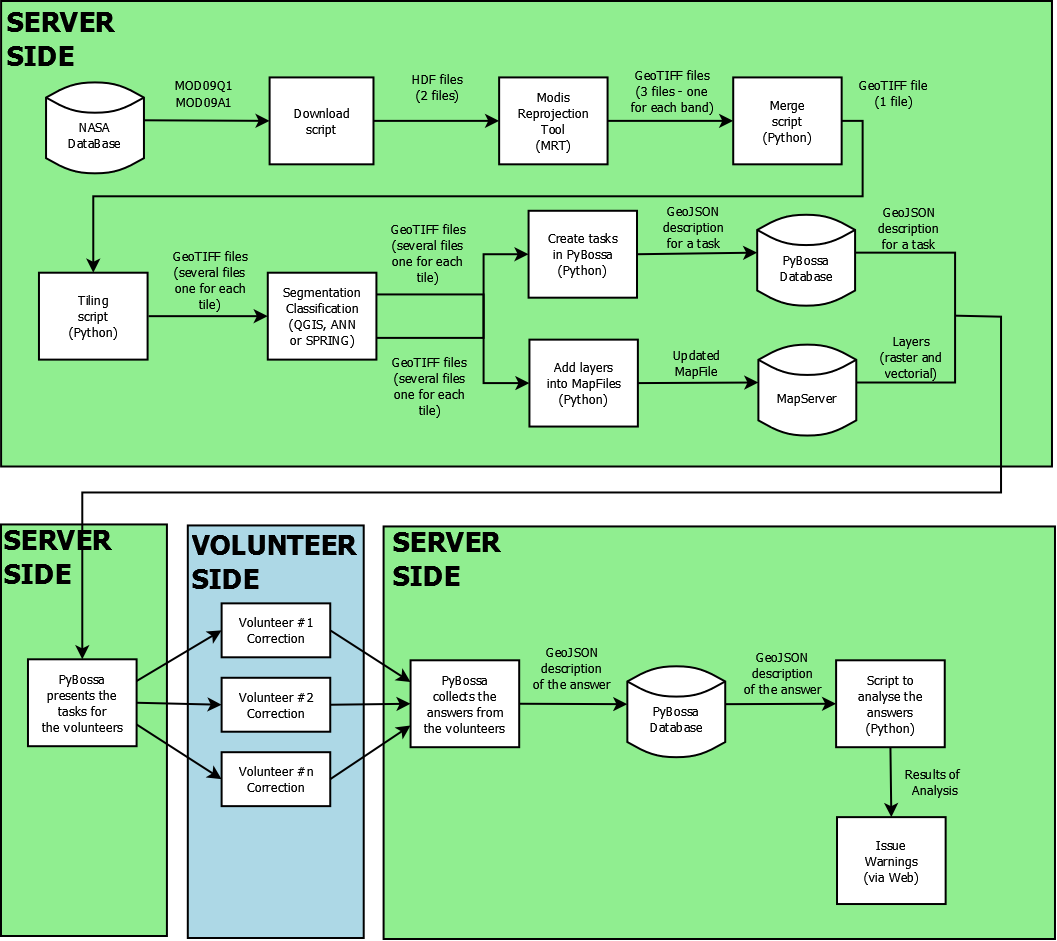
\includegraphics[width=\textwidth,height=\textheight,keepaspectratio]{figuras/arquitetura_atual.png}
\caption{A metodologia utilizada pelo projeto ForestWatchers.}
\label{fig:estrutura_atual}
\FONTE{\citeonline{ForestWatchersDesc}}
\end{figure}

Conforme a �rea do escopo do projeto, s�o selecionadas as imagens do cat�logo da NASA que possuam a menor cobertura de nuvens e a maior visibilidade do terreno. Para esse processo, ferramentas como FTP\footnote{\textit{File Transfer Protocol (FTP)} � um protocolo para transfer�ncia de arquivo utilizado na internet para efetuar \textit{downloads} e \textit{uploads} de arquivos.}e WGET\footnote{WGET � um programa livre para efetuar \textit{download} de conte�dos na internet.} s�o utilizadas para baixar as imagens. A pr�xima etapa, envolve recortar as imagens que n�o s�o pertinentes � �rea de interesse, descartando-as e consolidando as imagens restantes num �nico arquivo GeoTIFF de 16 bits. Essa etapa pode ser executada rapidamente com o aux�lio da ferramenta MODIS Reprojection Tool (MRT) \cite{MRToolManual2010}, um software gratuito disponibilizado pela NASA.

Assim, essa imagem pode ser enviada para um servidor que ir� gerenciar as imagens as serem dispon�veis em um software de Sistema de Informa��o Geogr�fica - SIG. O ForestWatchers utiliza o programa MapServer\footnote{\url{http://www.mapserver.org}} para mapas SIG, respons�vel por tratar as requisi��es de inser��o e sele��o das imagens georreferenciadas, e de retornar apenas parte da imagem desejada na forma de \textit{tiles}. Todos os arquivos relacionados � imagem t�m suas informa��es extra�das no formato GeoJSON\footnote{\textit{Geographic JavaScript Object Notation} � um formato para codificar variados tipos de estruturas geogr�ficas (Linhas, Pontos e Pol�gonos) utilizando a linguagem JavaScript.}, para facilitar a comunica��o entre os outros m�dulos.

Um algoritmo de classifica��o autom�tica de Rede Neural Artificial - RNA (em desenvolvimento cont�nuo) � respons�vel por segmentar as imagens, classificando-as como �reas de floresta e de n�o-floresta. Cada imagem resultada da classifica��o autom�ticas s�o subdivididas em imagens menores, que ser�o apresentadas aos volunt�rios como tarefas. As tarefas que ser�o apresentadas aos volunt�rios tem o intuito de corrigir ou validar a classifica��o autom�tica da RNA, o programa \citeonline{PyBossa2013} utilizado para gerenciar a cria��o e distribui��o das tarefas automaticamente, conforme necess�rio.

Esse � um sistema livre que permite criar e gerenciar projetos tais como classifica��o de imagem, transcri��o e geo codifica��o, que envolve tarefas de classifica��o supervisionada. Este � baseado no \citeonline{Boinc2008} criado por David P. Anderson, mesmo criador do projeto SETI@Home. A principal vantagem desta nova implementa��o em rela��o ao sistema original � o uso de uma \textit{API}\footnote{\textit{Application Programming Interface} (API) � um protocolo com o objetivo de servir como interface para os componentes de softwares, permitindo comunicarem entre si.} \textit{REST}\footnote{\textit{Representational State Transfer} (REST), em portugu�s Transfer�ncia de Estado Representacional \cite{Richardson2008}}.

Ap�s a cria��o das tarefas, os volunt�rios podem classificar as imagens de forma ordenada. O \citeonline{PyBossa2013} ainda pode ser configurado para agir como um sistema de redund�ncia de tarefas, podendo enviar a mesma tarefa para diferentes volunt�rios mais de uma vez, garantindo assim um aumento na confiabilidade dos resultados classificados pelos volunt�rios \cite{Ipeirotis2010}. A utiliza��o de tarefas redundantes em projetos de ci�ncia cidad� � uma das formas de aumentar a confiabilidade nos dados reportados.

Ao final das classifica��es das tarefas realizadas pelos volunt�rios, os resultados do projeto s�o disponibilizados no s�tio eletr�nico do ForestWatchers, podendo ser utilizados para gerar uma nova imagem levando em considera��o as respostas dos volunt�rios.

\chapter{METODOLOGIA}
\label{ch:metodologia}

O conceito de um m�dulo de sensoriamento volunt�rio consiste basicamente de \textbf{(a)} um dispositivo capaz de coletar dados, associado a uma \textbf{(b)} estrutura de recebimento e armazenamento, e a \textbf{(c)} um sistema de visualiza��o dos dados obtidos \cite{VolunteerSensing2011,Gouveia2008}.

Para o teste deste conceito o seguinte m�dulo foi constru�do em duas etapas. Primeiramente, um aplicativo h�brido, utilizado pelos volunt�rios para enviarem os dados coletados a partir de um dispositivo m�vel, foi desenvolvido. Em seguida, implementou-se uma infraestrutura tecnol�gica de camadas, divida em camada de recebimento, camada de armazenamento, camada de processamento e camada de visualiza��o dos dados.

Este cap�tulo descreve a metodologia utilizada em cada etapa da constru��o do m�dulo e detalha o experimento de coleta de dados utilizado para teste em condi��es reais do m�dulo.

\section{Aplicativos} % (fold)
\label{sub:aplicativos}

Tendo como foco o dispositivo de coleta de dados mais comum e geral poss�vel, de modo a aumentar o abrang�ncia do projeto FW, optou-se por desenvolver uma aplica��o para dispositivos m�veis do tipo (\textit{smartphones} e \textit{tablet}). Hoje, a grande maioria das pessoas possui um dispositivo m�vel com capacidade de conectar-se � internet, tirar fotos, captar �udio e gravar v�deos. Com a populariza��o dos sensores embarcados em dispositivos m�veis e as expectativas de crescimento deste mercado \cite{Lane2010,Gartner2014}, utiliz�-los como ferramenta para projetos de ci�ncia cidad� � uma abordagem natural.

Foram criados quatro aplicativos como prot�tipos para testar suas funcionalidades e verificar a sua signific�ncia em rela��o as necessidades do projeto: (i) um aplicativo utilizando bibliotecas nativas, disponibilizadas pelos fabricantes de dispositivos m�veis para criar novos aplicativos, como estes que s�o facilmente encontrados nas lojas online; (ii)  dois aplicativos baseados sistemas prontos ou de f�cil uso para a cria��o da ferramenta de coleta de dados; e por fim, (iii) um aplicativo utilizando uma abordagem de desenvolvimento de aplicativos h�brido, onde h� uma biblioteca em comum entre os demais dispositivos existentes e necessitando de apenas uma linguagem de programa��o.

Cada fabricante de dispositivos m�veis disponibiliza conjuntos de c�digos a serem utilizados para desenvolver aplicativos. Estes s�o conhecidos por biblioteca, \textit{Application Programming Interface} (API) ou \textit{Software Development Kit} (SDK). A maioria dos fabricantes fornecem essas bibliotecas sem custos, por�m, para poder publicar um aplicativo nas lojas online, alguns fabricantes requerem uma assinatura anual (Tabela \ref{tab:tabela_custo}).

Estas bibliotecas permitem desenvolver aplicativos para diversos dispositivos do mesmo fabricante. A Microsoft, por exemplo, permite criar aplicativos tanto para seus sistemas \textit{Desktop} (\textit{Windows}) quanto para aplicativos m�veis (Windows Phone e \textit{Tablets}). Outros fabricantes j� s�o mais restritivos e requerem a aquisi��o de uma outra licen�a para produtos diferentes, como a Apple para \textit{Desktop}, \textit{Smartphone} e \textit{Tablet}.

Na Tabela \ref{tab:tabela_custo}, as plataformas mostradas s�o referentes a pesquisa realizada por \citeonline{IDC:2014Q3}, onde aparecem somente as plataformas que foram mais consumidas de 2011 a 2014.

\begin{table}[htb]
\caption{Pre�o de Licen�a de Desenvolvimento por Plataforma.}
\label{tab:tabela_custo}
\resizebox{\textwidth}{!}{
    \begin{tabular}{@{}llll@{}}
    \toprule
    Plataformas                            & Dispositivos                            & Principal Linguagem & Licen�a  \\ \midrule
    iOS (Apple)                            & Smartphones, Tablets                    & Objective-C         & \$99/ano \\
    BlackBerry OS (RIM)                    & Smartphones                             & Java                & \$0      \\
    Windows 8, Windows Phone 8 (Microsoft) & Desktop, Smartphones, Tablets           & .NET                & \$19/ano \\
    Android (Google)                       & Acess�rio, Desktop, Smartphone, Tablets & Java                & \$25/ano \\ \bottomrule
    \end{tabular}
}
\FONTE{\citeonline{Registration:Android:2014,Registration:iPhone:2014,Registration:rim:2014,Registration:WP8:2014}}
\end{table}

%%%%%%%%%%%%%%%%%%%%%%%%%%%%%%%%5

\subsection{Aplicativo de Biblioteca Nativa}
\label{ssub:aplicativo_com_biblioteca_nativa}

O primeiro aplicativo desenvolvido como prot�tipo foi criado para a plataforma Windows Phone da Microsoft dada a disponibilidade de um \textit{smartphone} moderno, o Nokia Lumia 800, lan�ado no final de 2011\footnote{\url{http://www.gsmarena.com/nokia_lumia_800-4240.php}}. Este aparelho possui sensores de localiza��o (GPS assistido), aceler�metro, b�ssola, proximidade, c�mera de 8 megapixel com georreferenciamento, dentre outros. Um sensor de localiza��o GPS assistido tem a inicializa��o do seu servi�o mais r�pido do que um GPS convencional, pois pode utilizar informa��es de redes \textit{wireless} ou 3G para obter um melhor posicionamento inicial. Aceler�metros permitem monitorar a inclina��o do aparelho nos eixos X, Y e Z, fornecendo assim qual a posi��o do celular ao capturar uma imagem. C�meras com a habilidade de georreferenciamento permitem incluir informa��es geogr�ficas no cabe�alho de uma imagem, v�deo ou �udio, assim que estes s�o capturados. Este cabe�alho pode posteriormente ser lido e compreendido por outros softwares atrav�s do padr�o \textit{Exchangeable Image File Format} (EXIF) \cite{JEITA2002}.

Um simples aplicativo foi ent�o desenvolvido para capturar uma imagem utilizando a c�mera do dispositivo, guardar as coordenadas geogr�ficas atrav�s do georreferenciamento e envi�-las a um servidor, extraindo as informa��es necess�rias. Seu esquema de funcionamento � apresentado na Figura \ref{fig:wp7}.

\begin{figure}[htb]
\centering
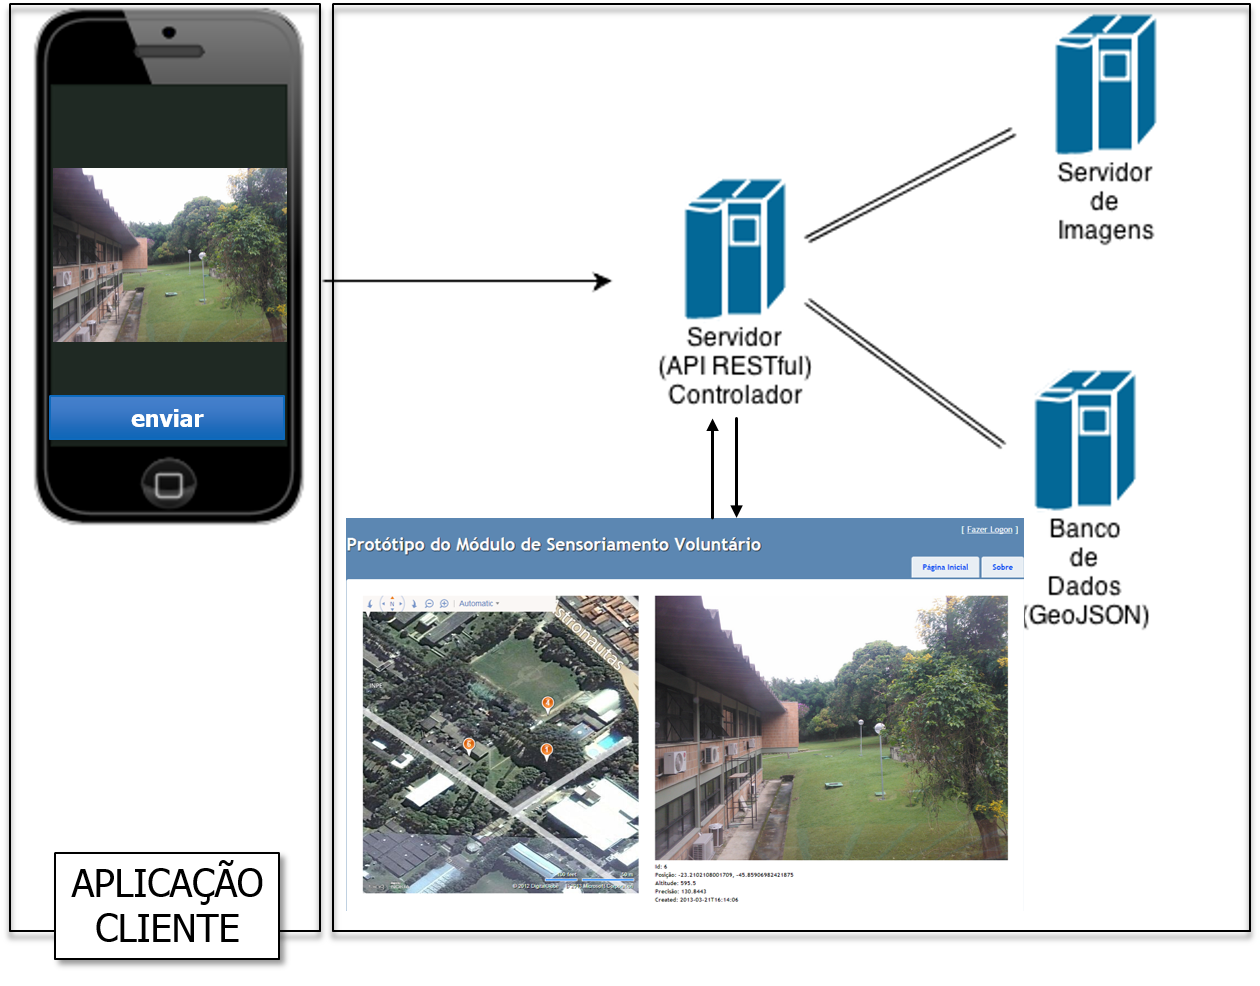
\includegraphics[keepaspectratio,width=0.9\textwidth]{figuras/prot_app_01.png}
\caption{Esquematiza��o do prot�tipo do aplicativo, incluindo uma aplica��o cliente, respons�vel por capturar a imagem e envi�-la ao servidor de atrav�s de REST. Os dados GeoJSON s�o armazenados no banco de dados e a imagem no servidor de imagens. Posteriormente, ao exibir a mesma imagem, a p�gina web faz a requisi��o da imagem e a requisi��o dos dados aos respectivos servidores, combinando seus resultados para exibi��o.}
\label{fig:wp7}
\end{figure}

Ao enviar o �nico arquivo contendo apenas a imagem capturada para o servidor, todas as informa��es do cabe�alho do arquivo s�o extra�das e armazenadas em um banco de dados geogr�fico, utilizando o formato GeoJSON \footnote{\url{http://geojson.org/}}. A imagem � armazenada em um diret�rio espec�fico, para que possa ser rapidamente lida e exibida em uma p�gina web. As primeiras imagens capturadas pelo aplicativo para teste do trabalho foram feitas de dentro do INPE em S�o Jos� dos Campos. Uma p�gina web foi criada para visualizar os resultados deste prot�tipo e, com esta, um mapa do sistema Bing\footnote{\url{http://www.bing.com/maps/}} foi utilizado para mostrar os imagens captadas sobrepostas como pontos de interesse. Ao clicar no �cone de cada ponto de interesse, a imagem correspondente � exibida com as suas informa��es de identifica��o de imagem do banco de dados, coordenada geogr�fica, altitude, precis�o e data de cria��o.

Alguns problemas foram detectados no uso deste prot�tipo, o que inviabilizou o seu uso. Estes s�o:

\begin{itemize}
    \item \textbf{Precis�o Geogr�fica}. Aparelhos \textit{smartphone}, em geral, n�o informam o n�vel de precis�o do georreferenciamento utilizado, tornando este aplicativo invi�vel. Erros de precis�o de GPS podem ser na ordem de quil�metros de dist�ncia do ponto original; \textit{smartphones} que possuem esta funcionalidade podem n�o captar uma posi��o geogr�fica por alguma falha e o usu�rio s� saber� posteriormente.
    \item \textbf{Georreferenciamento Automatizado}. Assim como n�o � poss�vel determinar a precis�o ou qualidade captada pelo sensor e que ser� georreferenciada na m�dia, tampouco � poss�vel prever que todas as m�dias (�udio, v�deo, imagens) de um \textit{smartphone} ser�o georreferenciadas automaticamente, uma vez que esta funcionalidade difere conforme a plataforma. O dispositivo Lumia 800 possui somente imagens georreferenciadas, por exemplo.
    \item \textbf{M�ltiplas Plataformas}. Aplicativos desenvolvidos para uma �nica plataforma atrair�o menos volunt�rios do que aplicativos desenvolvidos para mais de uma plataforma. Este � o ponto cr�tico para o desenvolvimento de aplicativos de sensoriamento volunt�rio.
\end{itemize}

\subsection{Aplicativo de Sistema Pronto}
\label{ssub:aplicativo_de_sistema_pronto}

{\centering
\begin{table}[htb]
     \label{tab:tipo_de_dados}
     \small
     \caption{Tipo de Dados Utilizados Pelo EpiCollect e EpiCollect+}
     \begin{center}
         \begin{tabular}{ p{2cm}  p{12cm}  }
             \toprule
              \tiny{Controle} & \tiny{Descri��o} \\
            \cmidrule(lr){1-1}\cmidrule(l){2-2}
             \raisebox{-0.5\height}{\centering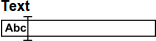
\includegraphics[scale=0.4]{figuras/epicollect/_input_text.png}}
                               &
              \tiny
                      Entrada de texto livre. Utilizado com maior frequ�ncia para responder perguntas feitas no formul�rio.
                                Op��es:

                                R�tulo. Exibi��o do texto como r�tulo;
                                Obrigat�rio. O usu�rio deve informar este dado;
                                Num�rico. Op��o para tornar o campo num�rico (EpiCollect).

              \\

             \raisebox{-0.5\height}{\centering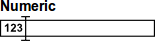
\includegraphics[scale=0.4]{figuras/epicollect/_input_numeric.png}}
              &
                                \tiny
                                Entrada de n�mero. Para o EpiCollect, um campo de entrada de texto com a op��o ``Num�rico'' deve ser selecionado para ter a mesma fun��o.
                                Op��es:

                                R�tulo. Exibi��o do texto como r�tulo.
                                Obrigat�rio. O usu�rio deve informar este dado.
                                Decimal. Permitindo casas decimais.
                                Inteiro. Permitindo somente entrada de n�meros inteiros.
                                Valor M�ximo. Valor m�ximo permitido para este campo.
                                Valor M�nimo. Valor m�nimo permitido para este campo.
                                Padr�o. Valor padr�o a ser especificado ao preencher o campo.
                                Entrada Dupla. O usu�rio deve entrar com o dado duas vezes para confirmar o seu valor.

                                \\

             \raisebox{-0.5\height}{\centering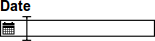
\includegraphics[scale=0.4]{figuras/epicollect/_input_date.png}}
              &
                                \tiny
                                Entrada de data. Este dado n�o possui para a vers�o do EpiCollect, apenas para o vers�o EpiCollect+.
                                \\

                                \raisebox{-0.5\height}{\centering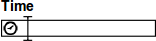
\includegraphics[scale=0.4]{figuras/epicollect/_input_time.png}}
                                &
                                \tiny
                                Entrada de Hora. Este dado n�o possui para a vers�o do EpiCollect, apenas para o vers�o EpiCollect+.
                                \\

             \raisebox{-0.5\height}{\centering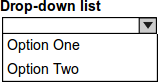
\includegraphics[scale=0.4]{figuras/epicollect/_input_dropdown.png}}
                                &
                                \tiny
                                Entrada de dados por sele��o. Este dado n�o possui para a vers�o do EpiCollect, apenas para o vers�o EpiCollect+.
                                Esta entrada permite escolher um valor atrav�s de uma lista.
                                Op��es:

                                R�tulo. Exibi��o do texto como r�tulo.
                                Obrigat�rio. O usu�rio deve informar este dado.

                                \\

             \raisebox{-0.5\height}{\centering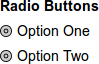
\includegraphics[scale=0.4]{figuras/epicollect/_input_radio.png}}
                                &
                                \tiny
                                Entrada de dados por sele��o. Este dado n�o possui para a vers�o do EpiCollect, apenas para o vers�o EpiCollect+.
                                Esta entrada permite escolher um valor atrav�s de uma lista, mostrando todos ao mesmo tempo.
                                Op��es:

                                R�tulo. Exibi��o do texto como r�tulo.
                                Obrigat�rio. O usu�rio deve informar este dado.

                                \\

             \raisebox{-0.5\height}{\centering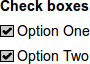
\includegraphics[scale=0.4]{figuras/epicollect/_input_checkbox.png}}
                                &
                                \tiny
                                Entrada de dados por sele��o. Este dado n�o possui para a vers�o do EpiCollect, apenas para o vers�o EpiCollect+.
                                Esta entrada permite escolher m�ltiplos valores atrav�s de uma lista, mostrando todos ao mesmo tempo.
                                Op��es:

                                R�tulo. Exibi��o do texto como r�tulo.
                                Obrigat�rio. O usu�rio deve informar este dado.

                                \\

             \raisebox{-0.5\height}{\centering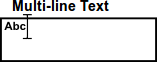
\includegraphics[scale=0.4]{figuras/epicollect/_input_multiline.png}}
                                &
                                \tiny
                                Entrada de texto.
                                \\

             \raisebox{-0.5\height}{\centering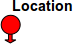
\includegraphics[scale=0.4]{figuras/epicollect/_input_location.png}}
                                &
                                \tiny
                                Entrada da coordenada geogr�fica. Este dado n�o possui para a vers�o do EpiCollect, apenas para o vers�o EpiCollect+.
                                Permite visualizar antes de salvar:

                                A coordenada geogr�fica atual.
                                A altitude da coordenada atual.
                                A orienta��o captada pela GPS atua.
                                A precis�o utilizada na capta��o dos dados acima.

                                \\

             \raisebox{-0.5\height}{\centering
\includegraphics[scale=0.4]{figuras/epicollect/_input_photo.png}}
                                &
                                \tiny
                                Entrada de foto. Este dado n�o possui para a vers�o do EpiCollect, apenas para o vers�o EpiCollect+.
                                Permite captar uma nova foto ou selecionar uma a partir da mem�ria do dispositivo.
                                \\

             \raisebox{-0.5\height}{\centering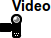
\includegraphics[scale=0.4]{figuras/epicollect/_input_video.png}}
                                &
                                \tiny
                                Entrada de v�deo. Este dado n�o possui para a vers�o do EpiCollect, apenas para o vers�o EpiCollect+.
                                Permite captar uma nova v�deo ou selecionar uma a partir da mem�ria do dispositivo.
                                \\

             \raisebox{-0.5\height}{\centering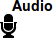
\includegraphics[scale=0.4]{figuras/epicollect/_input_audio.png}}
                                &
                                \tiny
                                Entrada de �udio. Este dado n�o possui para a vers�o do EpiCollect, apenas para o vers�o EpiCollect+.
                                Permite captar uma nova �udio ou selecionar uma a partir da mem�ria do dispositivo.
                                \\

             \raisebox{-0.5\height}{\centering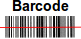
\includegraphics[scale=0.4]{figuras/epicollect/_input_barcode.png}}
                                &
                                \tiny
                                Entrada de c�digo de barra. Este dado n�o possui para a vers�o do EpiCollect, apenas para o vers�o EpiCollect+.
                                Permite decodificar um c�digo de barra ou c�digo QR.
                                \\

            \bottomrule
          \end{tabular}
      \end{center}
\end{table}
}

Com os problemas relatados anteriormente, buscou-se uma nova solu��o. H� diversos aplicativos que s�o desenvolvidos para uma determinada plataforma e posteriormente s�o migrados para uma outra plataforma, tornando-os multiplataforma. Com essa caracter�stica alguns aplicativos tornam-se poderosas ferramentas de coleta de dados, inclusive adicionando as informa��es de alguns dos sensores presentes no dispositivo. Algumas destas ferramentas utilizam formul�rios para guiar a coleta de dados, constru�dos atrav�s de interfaces gr�ficas de f�cil manipula��o. Estes sistemas prontos s�o indicados para efetuar a cria��o aplicativos voltado para pesquisas ou coleta de dados de uma forma r�pida, uma vez que possuem toda uma infraestrutura para armazenamento de dados e sua visualiza��o.

EpiCollect+ � a segunda gera��o de um conhecido sistema pronto. Esta nova vers�o possui diversos novos recursos \cite{Aanensen2009:epicollect}, como captura de  imagens, v�deos, �udios, localiza��o geogr�fica e leitura de c�digo de barra. Este sistema � de f�cil uso, bastando ter acesso � internet para que o usu�rio possa criar de um novo projeto, especificar a sua visibilidade (p�blico ou privado), definir se este poder� aparecer na p�gina da internet e criar um formul�rio (Figura \ref{fig:epicollect_formulario}).

\begin{figure}[htb]
\centering
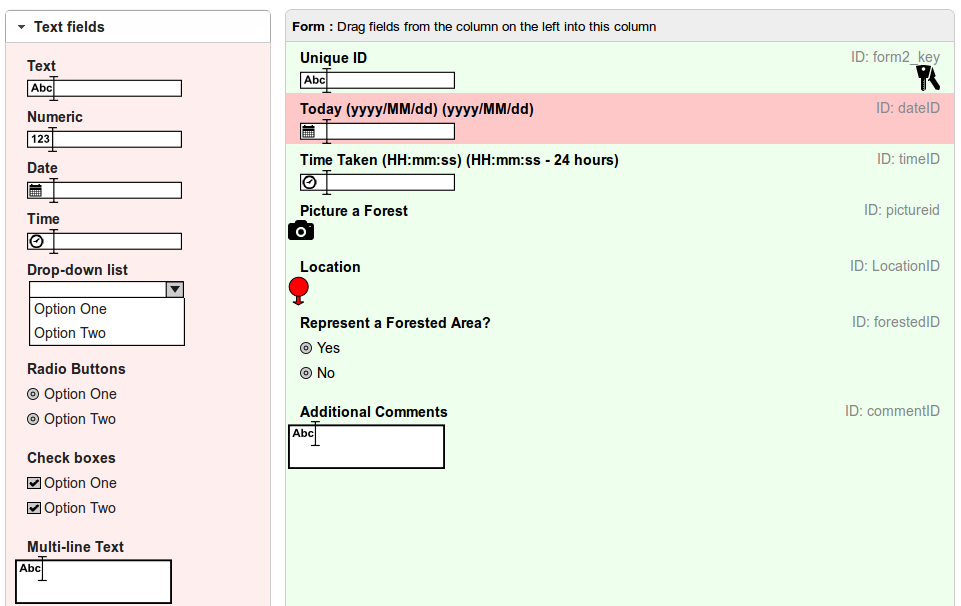
\includegraphics[keepaspectratio,width=0.7\textwidth]{figuras/epicollect/03_FORM_ANTIGO.png}
\caption{Um formul�rio criado para o EpiCollect+, com a finalidade de capturar uma imagem, foto ou v�deo, com a data e hora de aquisi��o, a coordenada geogr�fica e algum coment�rio adicional. }
\label{fig:epicollect_formulario}
\end{figure}

Esta segunda gera��o do aplicativo possui mais tipos de dados do que o primeiro, conforme observado na Tabela \ref{tab:tipo_de_dados}.

Um simples formul�rio foi criado (Figura \ref{fig:epicollect_formulario}) para verificar a viabilidade do sistema. Os dados do formul�rio s�o interpretados pelo PyBossa na fase de avalia��o Figura \ref{fig:pybossa_pertinente}, onde volunt�rios classificam as diversas imagens como pertinentes ao projeto (caso seja uma imagem de floresta, �rea sem floresta, etc.) ou n�o. Esta simples pergunta pode determinar o n�vel de comprometimento que um volunt�rio tem com o projeto, determinando se as imagens que este submete podem ser levadas em considera��o ou n�o.

\begin{figure}[htb]
\centering
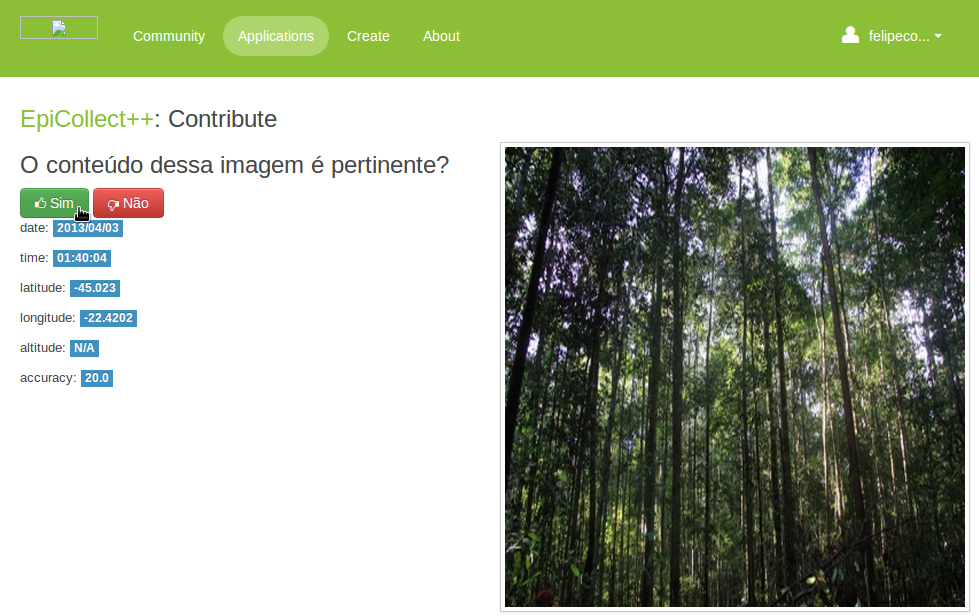
\includegraphics[keepaspectratio,width=0.7\textwidth]{figuras/_pertinencia.png}
\caption{Fase de avalia��o utilizando o sistema PyBossa para verificar a pertin�ncia da imagem em rela��o ao projeto.}
\label{fig:pybossa_pertinente}
\end{figure}

Uma vez que todos os dados foram capturados e os formul�rios corretamente preenchidos, estes s�o salvos e o volunt�rio pode inserir um novo registro ou efetuar a sincroniza��o com o servidor do EpiCollect+. A sincroniza��o pode tamb�m ser feita posteriormente, a crit�rio do volunt�rio, mantendo os dados de forma \textit{offline}.

O administrador do projeto pode verificar os dados online (Figura \ref{fig:epicollect_dados_online}) e us�-los localmente ap�s baixar os arquivos em csv\footnote{\textit{Comma-separted values} (csv) � um formato de arquivo cujos dados s�o separados por meio de v�rgulas.}, tsv\footnote{\textit{Tab-separted values} (tsv) � um formato de arquivo em que seus dados s�o separados por meio tabula��es.} ou xml\footnote{\textit{eXtensible Markup Language} (XML), um tipo de linguagem de marca��o.}, dependendo da necessidade.

\begin{figure}[htb]
\centering
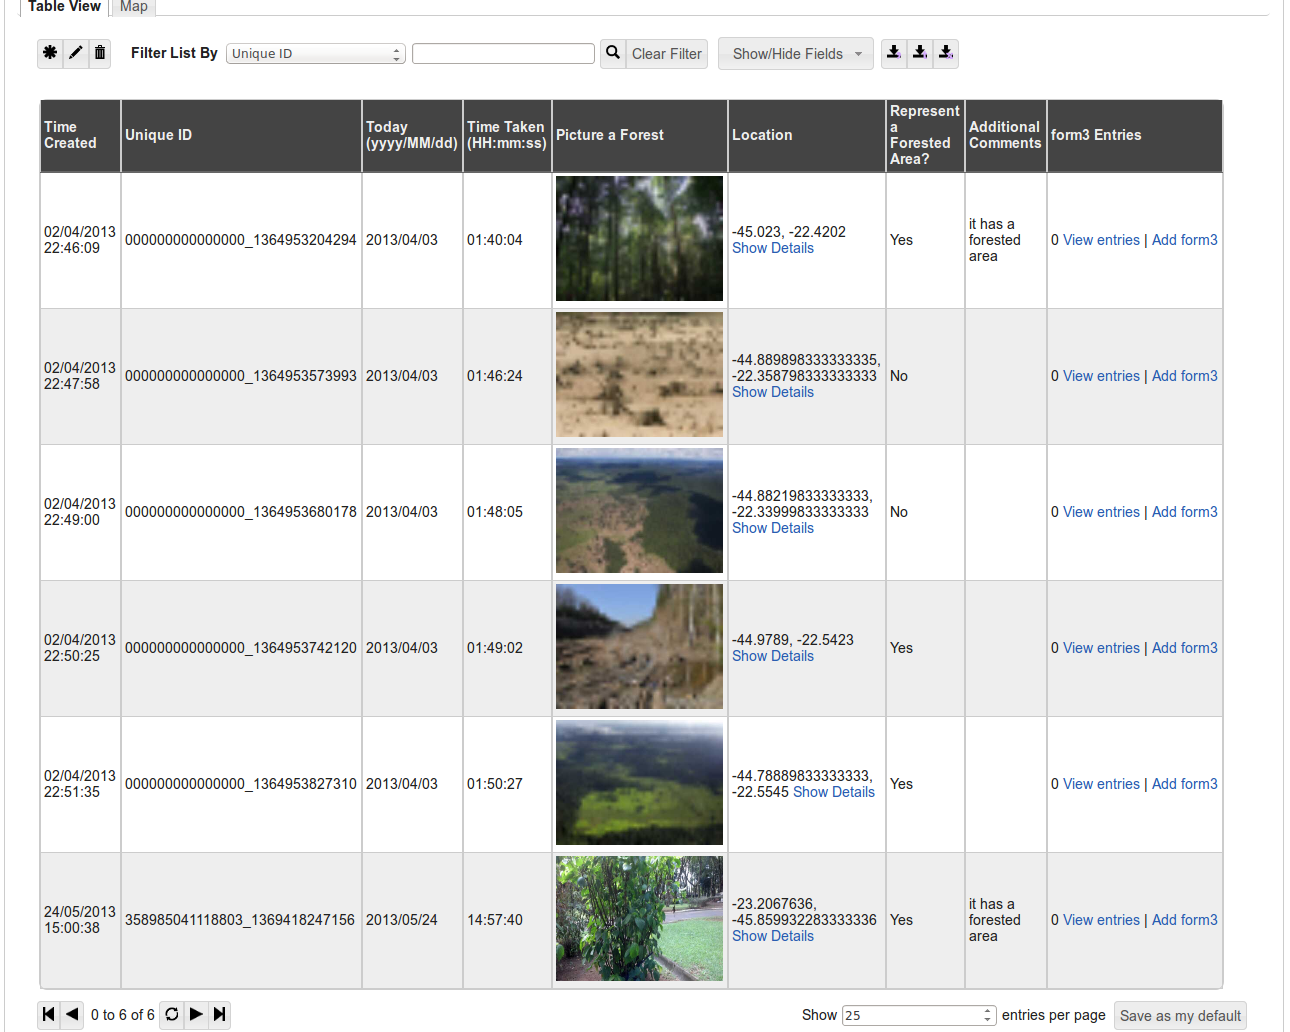
\includegraphics[keepaspectratio,width=0.7\textwidth]{figuras/epicollect/05_ALL_EPICOLLECT_DATA.png}
\caption{Os dados s�o mantidos nos servidores do EpiCollect+ para uso do administrador do projeto. }
\label{fig:epicollect_dados_online}
\end{figure}

Apesar de apresentar melhores solu��es para coletar diferentes tipos de dados, o EpiCollect+ possui apenas aplicativos para a plataforma Android. Assim como EpiCollect+, o Sensr tem a mesma fun��o de criar formul�rios online e atrav�s do seu aplicativo utiliz�-los como ferramenta de pesquisa. Por�m, assim como EpiCollect+, trabalha com uma �nica plataforma, o iOS.

\subsection{Aplicativo de Biblioteca H�brida}
\label{ssub:aplicativo_com_biblioteca_hibrida}

Em 1991 o primeiro s�tio eletr�nico foi criado, feito realizado por Berners-Lee em 1991 \cite{berners1992world}. Estima-se que em setembro de 2014 o n�mero de s�tios existentes chegou a marca de 1 bilh�o \cite{InternetLiveStats:2015}.

Os s�tios evolu�ram, deixaram de ser simples p�ginas est�ticas e passaram a ser mais din�micos. Hoje permitem que diversos usu�rios interajam ao mesmo tempo, efetuem pagamentos, realizem pesquisas e atualizem conte�do de forma simples. Estas novas funcionalidades s� foram alcan�adas atrav�s de grandes evolu��es das tecnologias empregadas no come�o da \textit{World Wide Web}. Existem diversas tecnologias de servidores para exibir um s�tio com conte�do din�mico, como PHP, .NET, Python, etc. HTML e CSS s�o as duas principais tecnologias para a constru��o de uma p�gina. O HTML define a estrutura da p�gina e permite o uso de fotos, formul�rios, links, v�deos, �udios, tabelas, etc. O CSS descreve o layout da p�gina com cores, posi��es e fontes. Uma p�gina tamb�m pode utilizar \textit{scripts} (o mais conhecido, JavaScript) de forma a torn�-la mais expressiva, dando dinamicidade ao seu conte�do, com valida��es e, at� mesmo, carregamento de conte�do din�mico.

HTML, CSS e JavaScript s�o conhecidos por serem os pilares para uma p�gina moderna. Estes s�o padronizados pela \textit{World Wide Web Consortium} (W3C). Criado por Berners-Lee em 1994, este cons�rcio � constitu�do por quase 400 membros, como empresas, �rg�os governamentais e organiza��es independentes, todos com a finalidade de estabelecer padr�es para a cria��o e a interpreta��o de conte�dos para a Web. Sem a exist�ncia destes padr�es, haveria diversos navegadores para a internet, cada um interpretando uma determinada p�gina de forma diferente do outro, tendo o usu�rio que trocar de navegador a cada nova navega��o.

O desenvolvimento de aplicativos utilizando bibliotecas nativas s�o mais comuns, por poderem usufruir de todas as funcionalidades oferecidas pelos fabricantes de dispositivos m�veis e tamb�m por serem mais r�pidos \cite{Charland:2011:Mobile}. Entretanto esta forma de desenvolvimento de aplicativos pode n�o ser vantajosa para um desenvolvedor que busca alcan�ar o m�ximo de pessoas poss�vel. Neste caso � melhor que o aplicativo seja desenvolvido de todas as plataformas poss�veis (ver Figura \ref{fig:developerforce}).

\begin{figure}[ht]
\begin{center}
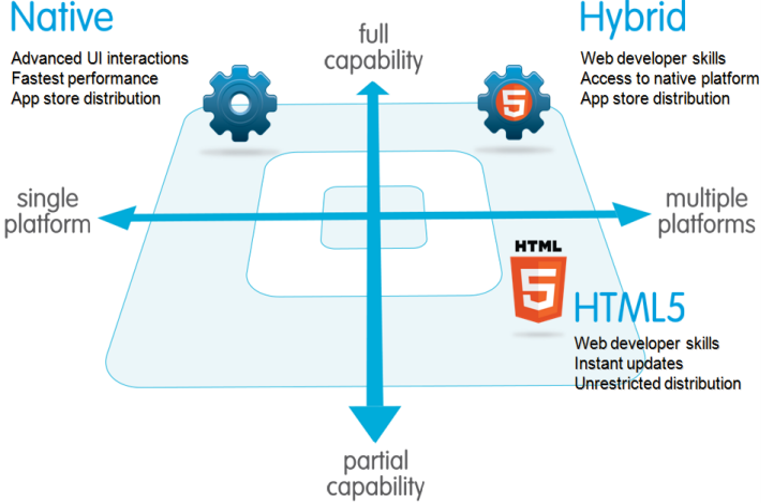
\includegraphics[keepaspectratio,width=0.7\textwidth]{figuras/developerforce_chart.png}
\end{center}
\caption{Aplicativos m�veis podem ser desenvolvidos de tr�s formas: com biblioteca Nativa (plataforma �nica); HTML5 (multiplataforma e capacidade parcial); e H�brida (multiplataforma e capacidade total).}
\FONTE{\citeonline{Korf2013}}
\label{fig:developerforce}
\end{figure}

Todas as plataformas permitem que um desenvolvedor instancie um navegador dentro da sua aplica��o de forma que este passe a se comportar como uma nova tela nativa da aplica��o. Estas ainda permitem a intera��o de c�digos nativos atrav�s da utiliza��o de JavaScript. Esta t�cnica foi utilizada pela primeira vez por Eric Oesterle, Rob Ellis, e Brock Whitten para a plataforma iOS, depois sendo portado para outras plataformas \cite{Charland:2011:Mobile}. O \textit{framework} de c�digo aberto para o desenvolvimento de aplicativos h�bridos conhecido por PhoneGap foi fruto desta t�cnica. Em 2011 a empresa Adobe\footnote{\url{http://www.adobe.com}} adquiriu a criadora deste \textit{framework}, Nitobi, mantendo-o como c�digo aberto \cite{Adobe:Nitobi:2011}. O PhoneGap foi ent�o doado para a Funda��o de Software Apache sob o nome de Apache Cordova\footnote{\url{http://cordova.io/}}. O prop�sito desta mudan�a foi o de manter o c�digo sempre aberto e em constante desenvolvimento \cite{PhoneGap:FAQ:2015}.

A rela��o de PhoneGap e Cordova pode parecer confusa, por�m a Adobe esclarece que o PhoneGap � apenas uma distribui��o livre do cordova, geralmente logo na vers�o mais atualizada deste �ltimo \cite{PhoneGap:FAQ:2015}.

Na sua vers�o mais atual, PhoneGap 4.0.0, existem mais de nove plataformas suportadas\footnote{\url{http://cordova.apache.org/contribute}}. Algumas das principais podem ser vistas na Figura \ref{fig:phonegap_platforms}. Entre estas est�o as plataformas citadas na Tabela \ref{tab:tabela_custo}. As principais funcionalidades encontradas nas bibliotecas nativas est�o tamb�m presentes no PhoneGap (ver Fig. \ref{fig:phonegap_platforms}). A partir da vers�o 3.0 e superior, o PhoneGap oferece estas funcionalidades atrav�s de plugins que podem ser obtidos na p�gina do projeto Cordova.

\begin{figure}[ht]
\begin{center}
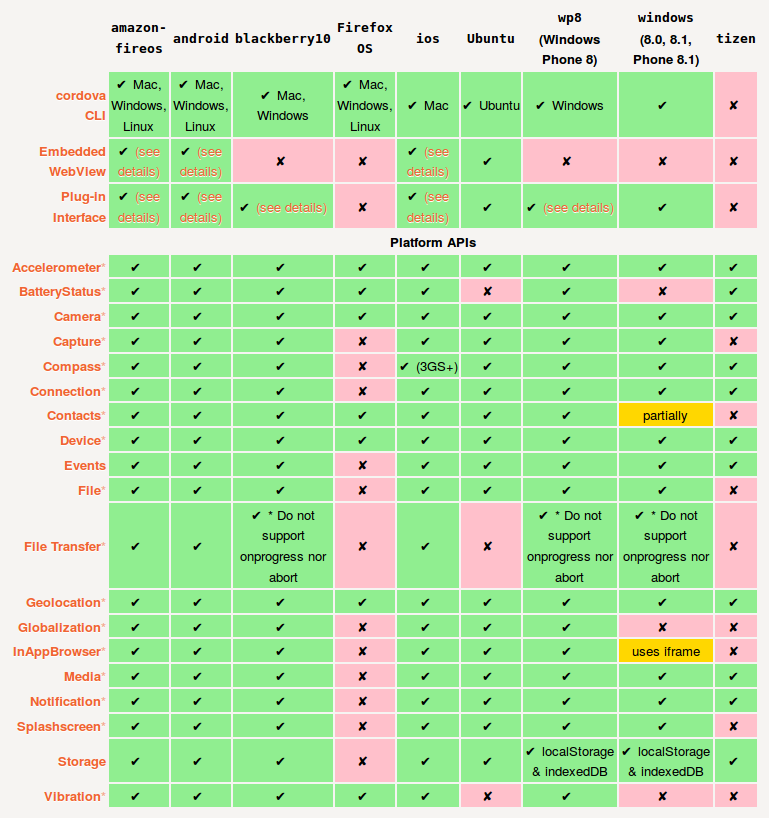
\includegraphics[keepaspectratio,width=0.7\textwidth]{figuras/phonegap_platforms.png}
\end{center}
\caption{Plataformas e funcionalidades suportadas pela vers�o 4.0.0 do PhoneGap. As funcionalidades com um asterisco s�o suportadas atrav�s de \textit{plugins} de terceiros \cite{PhoneGap:PlatformSupport:2015}.}
\label{fig:phonegap_platforms}
\end{figure}

Estes plugins permitem que apenas as funcionalidades desejadas sejam integradas ao aplicativo. Desta forma � poss�vel manter o desenvolvimento de uma aplica��o modular, tendo diversos plugins em diversas aplica��es cada qual com diferentes vers�es. Portanto, n�o h� mais a necessidade de atualizar todo o conjunto, apenas atualizar o plugin necess�rio e para a vers�o necess�ria.

Um plugin refere-se a uma funcionalidade espec�fica do dispositivo a ser encapsulado por um c�digo JavaScript para sua utiliza��o pelo framework PhoneGap. Em termos de Programa��o Orientada a Objetos, a biblioteca JavaScript deste framework tem a funcionalidade de uma interface, na qual s�o definidas as chamadas aos m�todos que ser�o utilizados. A implementa��o destas funcionalidades � feita a n�vel de plataforma, de modo a obter a funcionalidade desejada pela interface que a invocou, Figura \ref{fig:phonegap_layers}.

\begin{figure}[htb]
\begin{center}
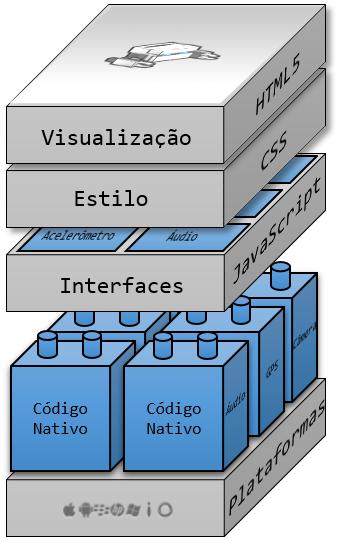
\includegraphics[scale=0.8]{figuras/layers.png}
\end{center}
\caption{A partir da vers�o 3.0, o framework PhoneGap vem utilizando plugins para adicionar diversas funcionalidades aos aplicativos. A camada de visualiza��o � composta por HTML5 e CSS, enquanto a camada l�gica � composta pelo JavaScript do framework \cite{PhoneGap:CommandLine:2015}.}
\label{fig:phonegap_layers}
\end{figure}

Diversos novos plugins podem ser desenvolvidos cobrindo novas funcionalidades, novos sensores e para novas plataformas. O PhoneGap mant�m 19 plugins para as funcionalidades de bateria, c�mera e �udio, GPS e sensores de movimento, conex�o, contatos, dispositivo, arquivos e armazenamento, notifica��o e transfer�ncia de arquivos (ver Fig. \ref{fig:phonegap_platforms}) . Por�m, na p�gina oficial\footnote{\url{http://plugins.cordova.io}}, podem ser encontrados outros 678 diferentes plugins, alguns executando funcionalidades semelhantes e outros ampliando as plataformas suportadas.

Existem duas frentes para se desenvolver com o PhoneGap. A primeira � atrav�s do uso de ambientes de desenvolvimento propriet�rios (Android Studio, Visual Studio, XCode, etc), onde um projeto PhoneGap para determinada plataforma � carregado e onde todo o desenvolvimento � realizado.

A segunda frente de desenvolvimento � atrav�s de linhas de comando. Ap�s a instala��o do framework PhoneGap, este permite compilar para mais de uma aplica��o simultaneamente utilizando apenas linhas de comando. Assim, um desenvolvedor que possui as ferramentas de desenvolvimento para iOS e Android, por exemplo, pode compilar seu aplicativo para ambos apenas atrav�s de simples instru��es digitados no terminal.

Como um aplicativo PhoneGap possui plugins e utiliza o JavaScript de interface para acessar suas funcionalidades, o desenvolvedor precisa manter apenas o HTML5, CSS e JavaScript uma �nica vez. Estes ser�o replicados para as outras plataformas conforme solicitado atrav�s de linha de comando.

Com uma funcionalidade extra, PhoneGap Build\footnote{\url{http://build.phonegap.com}}, o PhoneGap permite que seus usu�rios compilem seus aplicativos para mais de uma plataforma pela internet. Utilizando linhas de comando ou atrav�s de um arquivo zip que contenha os arquivos HTML, CSS e JavaScript necess�rios, o PhoneGap Build disponibiliza rapidamente um novo aplicativo compilado. Este ainda permite incluir a chave de acesso de desenvolvedor das demais plataformas, gerando assim um aplicativo pronto para inserir nas lojas de aplicativos existentes.

Para o projeto FW foi criado um aplicativo h�brido com o framework PhoneGap. Este aplicativo utilizou jQueryMobile (jQM)\footnote{\url{http://jquerymobile.com/}} para construir a interface gr�fica. jQM � um framework baseado em HTML5, CSS e JavaScript para construir interfaces gr�ficas para dispositivos m�veis. Junto com este \textit{framework}, utilizou-se a biblioteca KnockoutJS\footnote{\url{http://knockoutjs.com/}}, um \textit{framework} baseado em JavaScript para o uso de padr�es de projeto do tipo \textit{Model-View-ViewModel} (MVVM).

A Figura \ref{fig:UMLApplicationUseCase} ilustra o caso de uso do prot�tipo desenvolvido, onde o volunt�rio � um dos atores dos casos de uso. O volunt�rio pode capturar imagem, �udio e v�deo, que s�o recursos do sistema. Ap�s capturar um recurso, automaticamente � solicitado ao volunt�rio selecionar um dos dados retornados de GPS e orienta��o (caso exista b�ssola no dispositivo).

\begin{figure}[h]
\centering
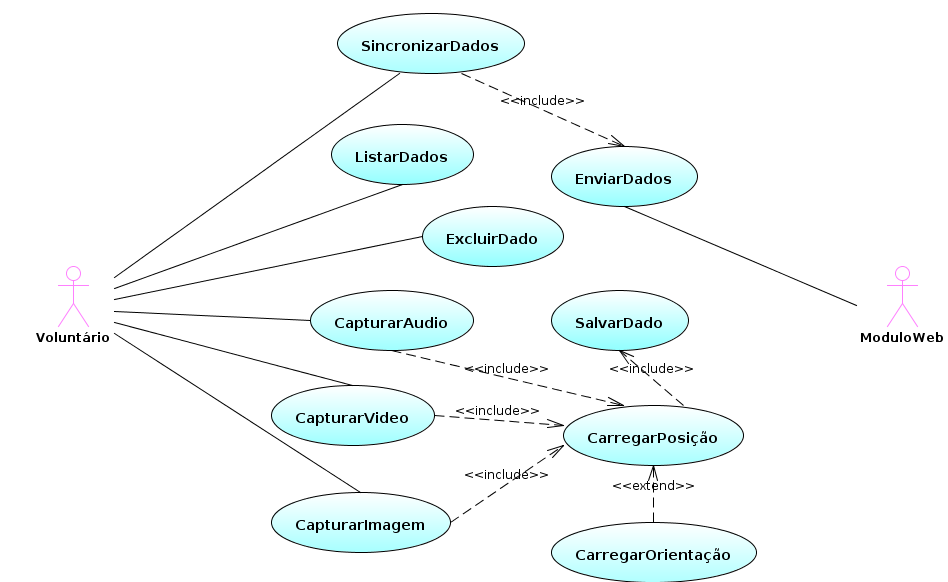
\includegraphics[width=0.9\textwidth]{figuras/UML/UMLApplicationUseCase.png}
\caption{Caso de uso do aplicativo desenvolvido para o projeto. O ator deste caso de uso, o volunt�rio, pode capturar �udios, v�deos e imagens. Em conjunto com estes dados, podem ser capturados ainda a posi��o geogr�fica e a sua orienta��o.}
\label{fig:UMLApplicationUseCase}
\end{figure}

O aplicativo, com o fluxo apresentado na Figura \ref{fig:app_phonegap}, � capaz de capturar imagem, v�deo e �udio, dados dos sensores de localiza��o (GPS) e orienta��o (b�ssola). Este aplicativo foi desenvolvido para permitir que no momento da captura dos dados de localiza��o e orienta��o, o usu�rio pudesse verificar o n�vel de precis�o dos dados coletados e, se necess�rio, captar novamente.

\begin{figure}[h]
\centering
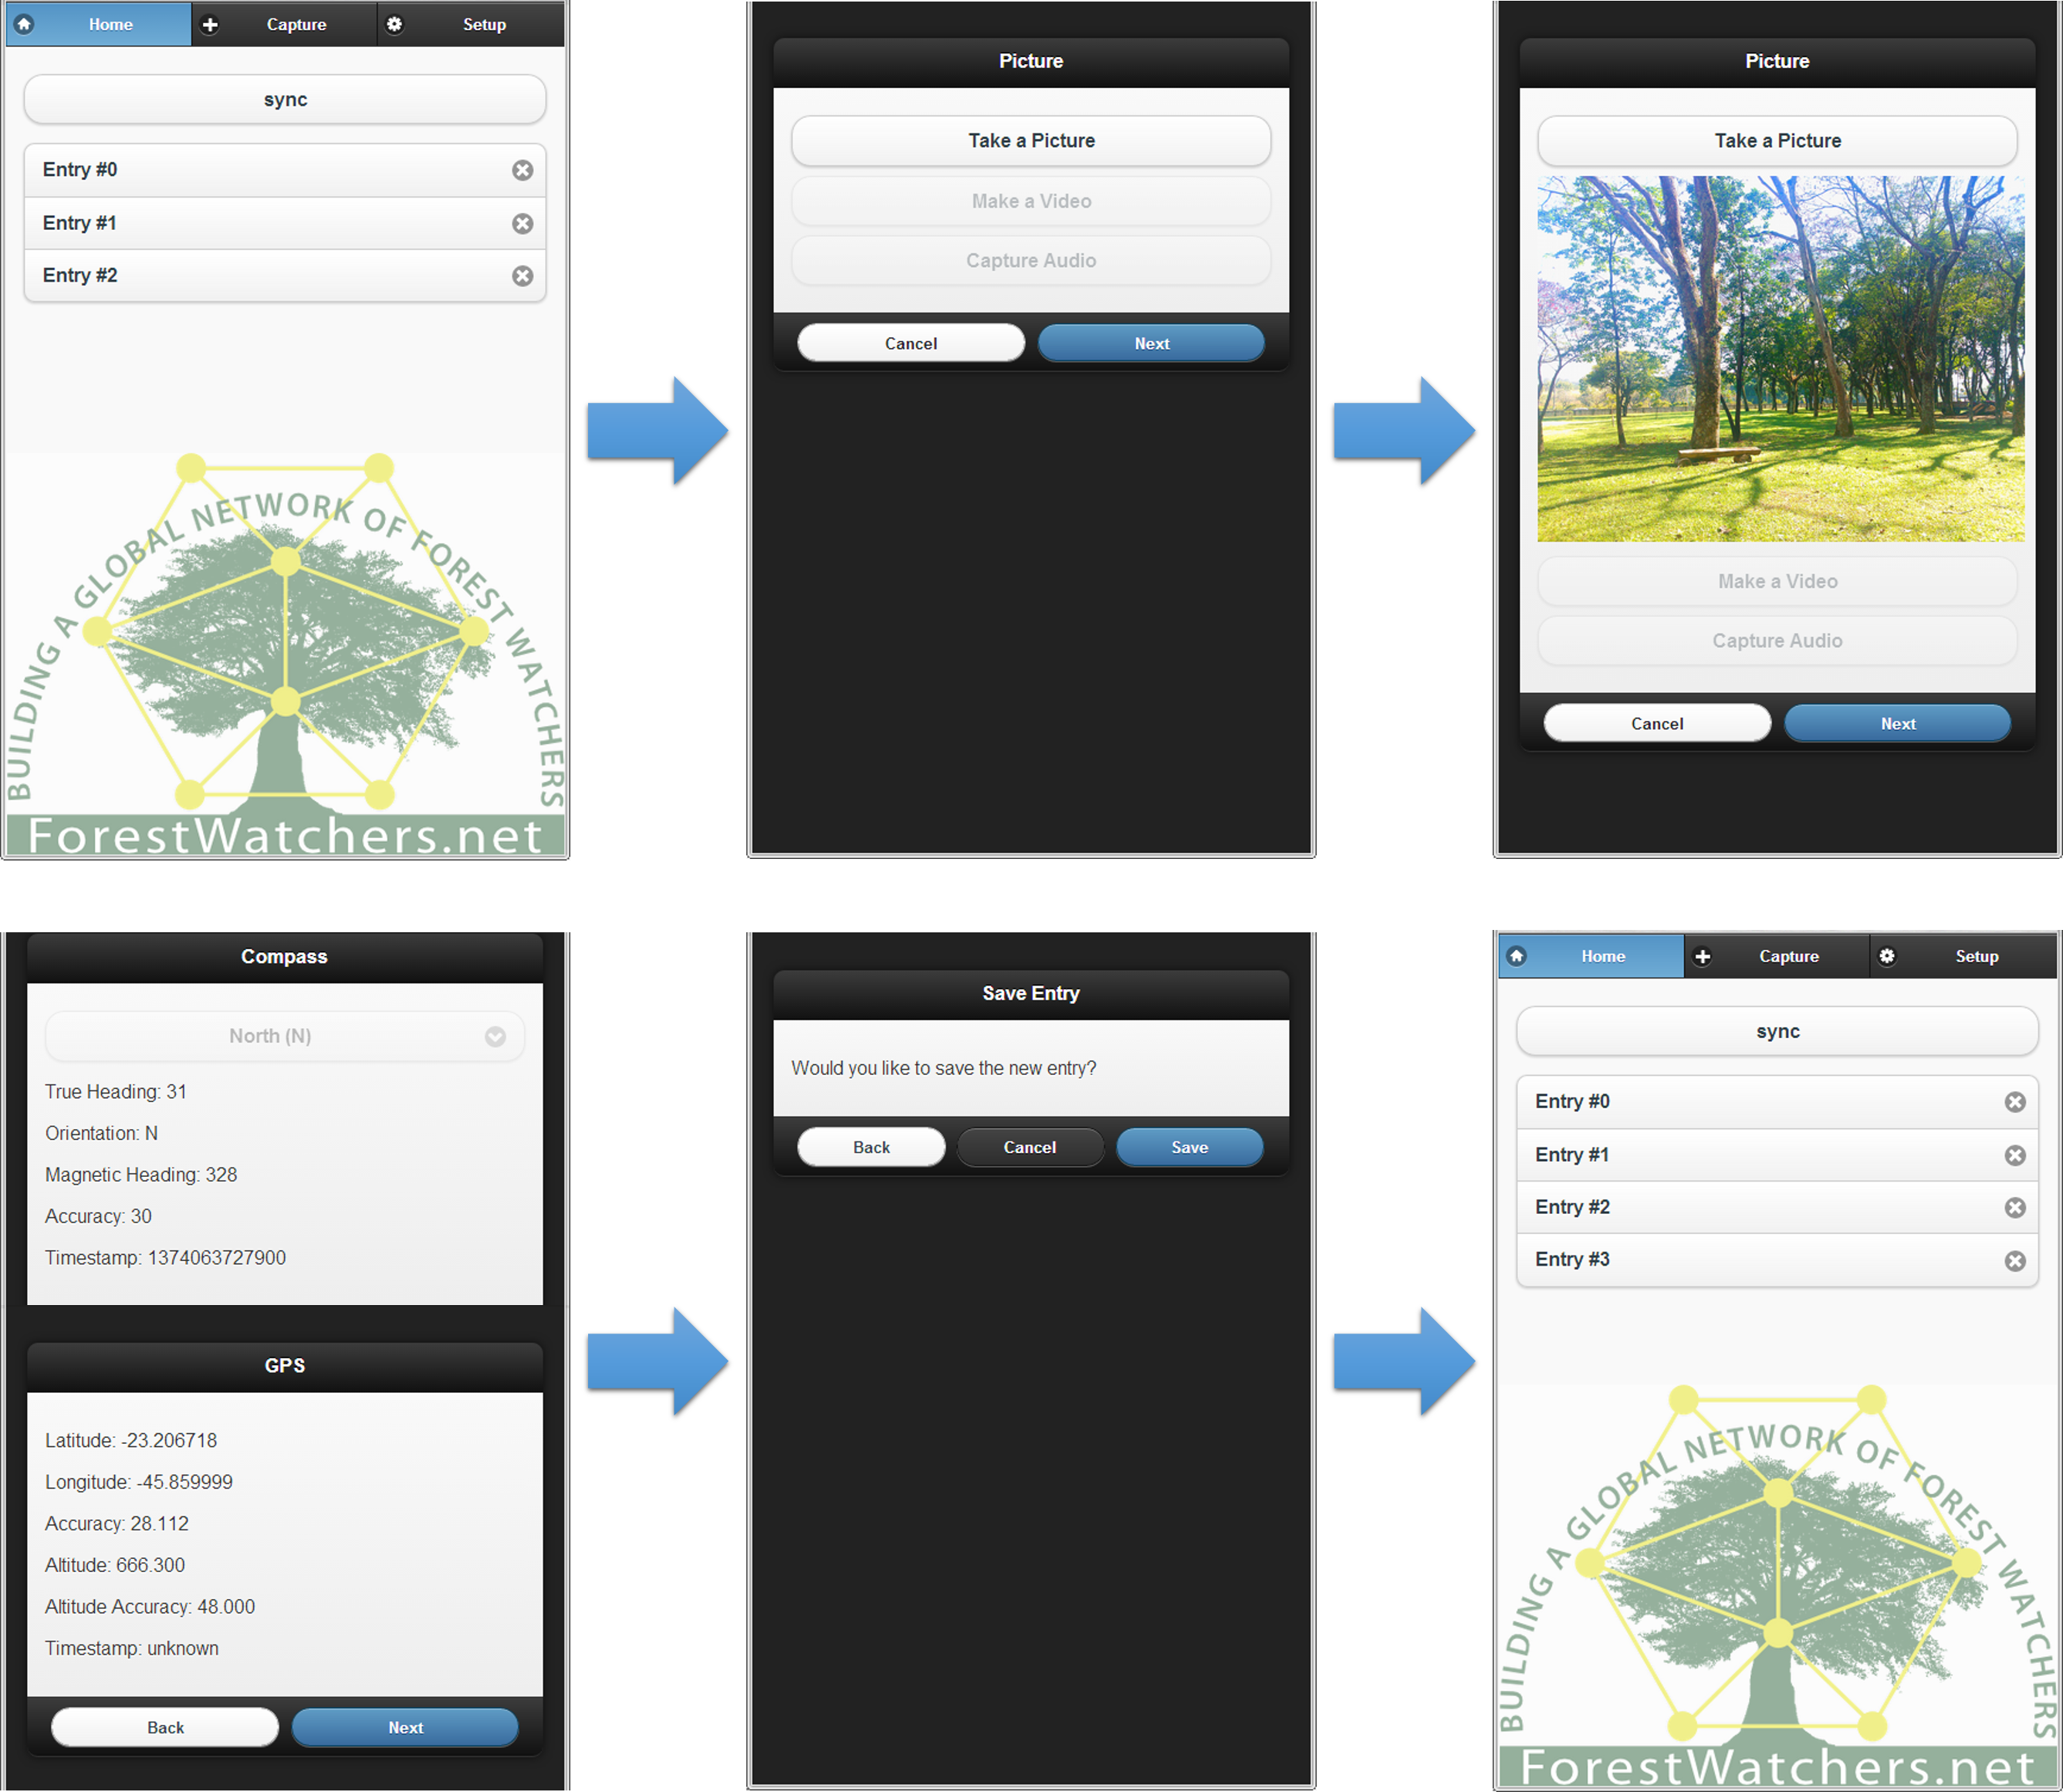
\includegraphics[width=0.7\textwidth]{figuras/dev_app04.png}
\caption{O aplicativo desenvolvido para este projeto baseado em Phonegap. A figura ilustra o fluxograma da captura de uma imagem, adquirindo informa��es extras do sensor de localiza��o (GPS) e do sensor de orienta��o (b�ssola magn�tica).}
\label{fig:app_phonegap}
\end{figure}

A Figura \ref{fig:UMLApplicationCaptureImageSequence} ilustra a sequ�ncia de a��es feitas para capturar uma imagem utilizando o aplicativo criado.

\begin{figure}[h]
\centering
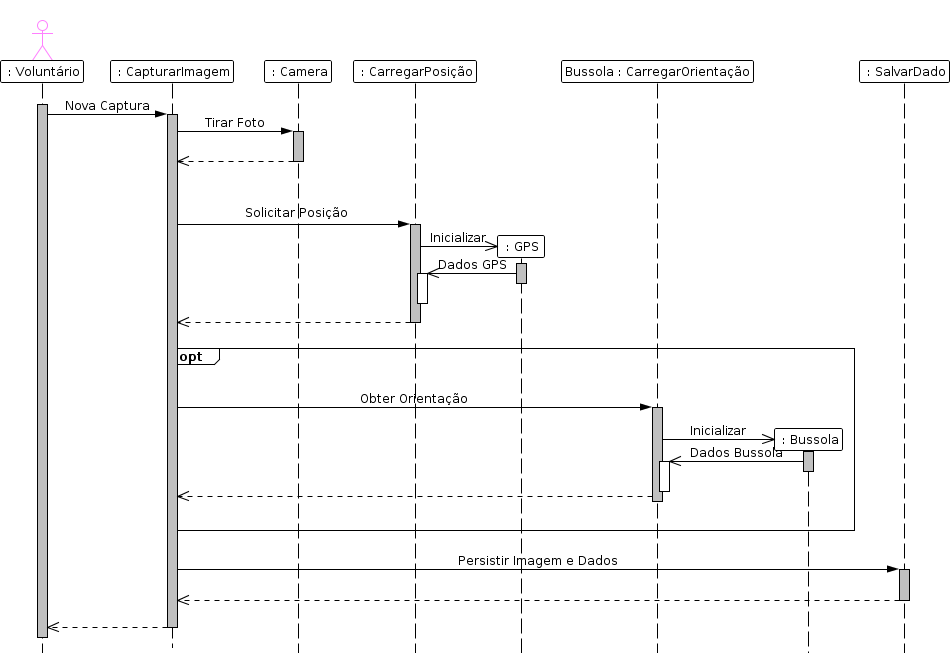
\includegraphics[width=0.9\textwidth]{figuras/UML/UMLApplicationCaptureImageSequence.png}
\caption{Diagrama de sequ�ncia ao utilizar o programa para capturar uma imagem, �udio ou v�deo.}
\label{fig:UMLApplicationCaptureImageSequence}
\end{figure}

Os dados captados por este aplicativo s�o em geral dados dos sensores de localiza��o (GPS), orienta��o (b�ssola), informa��es do dispositivo e informa��es do arquivo capturado. Estes dados podem ser verificados na Tabela \ref{tab:dados_captados}, onde as principais propriedades s�o listadas. Dados sobre a configura��o de cada sensor tamb�m s�o armazenados, mas apenas para refer�ncia. Diversos outros dados poderiam ser captados, mas para um primeiro prot�tipo apenas estes foram utilizados.

\begin{table}[h]
\centering
\small
\caption{Sum�rio dos Dados Gravados pelo Aplicativo}
\label{tab:dados_captados}
\resizebox{\textwidth}{!}{
\begin{tabular}{@{}lll@{}}
\toprule
\textbf{Contexto}    & \textbf{Propriedade} & \textbf{Descri��o}                         \\ \midrule
\textbf{}            &                      &                                            \\
\textbf{Entrada}     & Nome do Arquivo      & Nome do arquivo gerado                     \\
\textbf{}            & Caminho do Arquivo   & Local do armazenamento do arquivo          \\
\textbf{}            &                      &                                            \\
\textbf{B�ssola}     & Norte Verdadeiro     & Valor captado do Norte Verdadeiro          \\
\textbf{}            & Norte Magn�tico      & Valor captado do Norte Magn�tico           \\
\textbf{}            & Posi��o              & Uma posi��o, seguindo a rosas do vento     \\
\textbf{}            & Sele��o Manual       & Posi��o selecionada por sensor ou manual   \\
\textbf{}            & Precis�o             & Valor da precis�o captada                  \\
\textbf{}            &                      &                                            \\
\textbf{GPS}         & Latitude             & Posi��o geogr�fica da paralela horizontal  \\
\textbf{}            & Longitude            & Posi��o geogr�fica da paralela horizontal  \\
\textbf{}            & Precis�o             & Valor da precis�o captada                  \\
\textbf{}            & Altura               & Altura registrada pelo sensor              \\
\textbf{}            & Precis�o da Altura   & Valor da precis�o da altura quando captada \\
\textbf{}            & Dire��o              & Dire��o sugerida pelo sensor               \\
\textbf{}            & Velocidade           & Velocidade sugerida pelo sensor            \\
\textbf{}            &                      &                                            \\
\textbf{Dispositivo} & UUID                 & N�mero de identifica��o �nico              \\
\textbf{}            & Vers�o               & Vers�o do sistema operacional              \\
\textbf{}            & Cordova              & Vers�o do cordova                          \\
\textbf{}            & Plataforma           & Plataforma utilizada                       \\
\textbf{}            & Modelo               & Modelo utilizado                           \\ \bottomrule
\end{tabular}
}
\end{table}

A sincroniza��o dos dados entre dispositivo e servidor n�o precisa ocorrer ao mesmo tempo em que as entradas s�o captadas j� que muitas vezes quem ir� utilizar o aplicativo estar� em lugares remotos. Neste caso, as informa��es captadas s�o mantidas apenas no dispositivo para uma sincroniza��o futura e de prefer�ncia atrav�s de WiFi, uma vez que arquivos de v�deos podem ser bem maiores do que uma foto.

O conjunto de entradas � armazenado no dispositivo atrav�s do plugin de armazenamento interno, que permite persistir objetos no formato JSON. Estes dados permanecer�o no dispositivo at� que o usu�rio escolha a op��o de remover as entradas, caso este j� tenha sincronizado os dados com o servidor. A estrutura de uma �nica entrada � exibida no C�digo \ref{json:estrutura_imagem} do Ap�ndice A.

\section{Infraestrutura Tecnol�gica}
\label{sub:infraestrutura_tecnologica}

A infraestrutura para receber, armazenar e exibir os dados coletados pelos volunt�rios baseou-se em tecnologias de c�digo aberto. A finalidade � obter-se uma plataforma de distribui��o livre juntamente com seu c�digo fonte, podendo ser enriquecido por outros trabalhos.

A Figura \ref{fig:ArquiteturaServidores} ilustra a infraestrutura que foi criada para atender as necessidades deste m�dulo.

\begin{figure}[h]
\centering
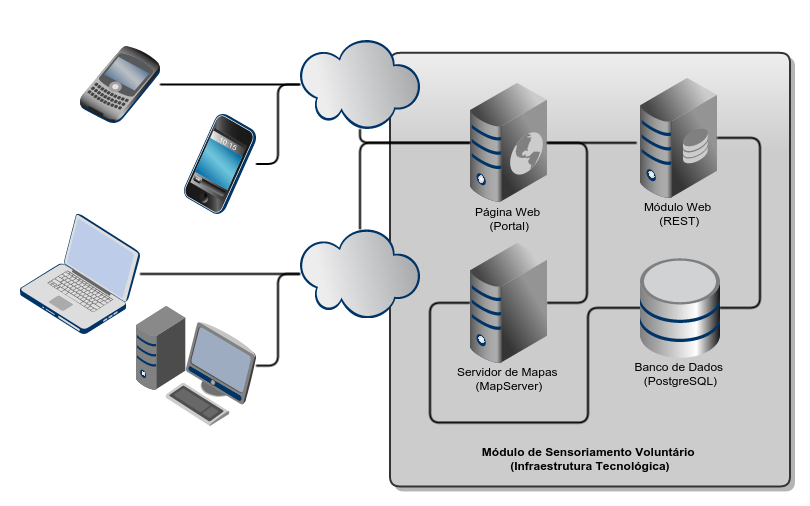
\includegraphics[width=0.7\textwidth]{figuras/UML/ArquiteturaServidores.png}
\caption{A arquitetura desenvolvida para o projeto, envolve um servidor de p�ginas web, um m�dulo web para receber os dados enviados pelos volunt�rios, um servidor de mapas respons�vel por informar dados geogr�ficos e um banco de dados para armazenar dados espaciais.}
\label{fig:ArquiteturaServidores}
\end{figure}

\subsection{Servidor para Internet}
\label{sub:servidor_web}

Duas s�o as principais tecnologias por tr�s deste projeto. A primeira, o aplicativo para dispositivos m�veis, � respons�vel por coletar os dados dos volunt�rios; a segunda, o servidor para internet, recebe os dados coletados pelos volunt�rios, armazena-os adequadamente e exibe-os quando solicitado.

Para a constru��o da aplica��o web, foi utilizado um \textit{framework} criado em Python para construir p�ginas, aplica��es e servi�os para a internet, Flask\footnote{\url{http://flask.pocoo.org/}}. Este \textit{framework} permite a constru��o de solu��es para internet de forma r�pida por possuir um grande reposit�rio de extens�es.

Utilizando Flask foi poss�vel desenvolver um servidor \textit{back-end} respons�vel por receber os dados enviados pelos volunt�rios e ao mesmo tempo um servidor \textit{front-end} respons�vel por mostrar os dados recebidos no formato de uma p�gina web, a interface da plataforma.

\subsubsection{Back-End}
\label{ssub:back_end}

O principal meio de comunica��o com servidores web � atrav�s do protocolo \textit{Hypertext Transfer Protocol} (HTTP), em portugu�s Protocolo de Transfer�ncia de Hipertexto. Este funciona por meio de requisi��o e resposta, como cliente e servidor. Um usu�rio que deseja visualizar uma p�gina da internet faz uma requisi��o ao servidor para obter o conte�do desejado, de forma autom�tica atrav�s do navegador.

Uma p�gina, definida pelo endere�o \url{http://www.inpe.br/pos_graduacao/cursos/cap/index.php}, � um recurso do servidor \url{www.inpe.br}. Para obter este recurso � necess�rio efetuar uma requisi��o (C�digo \ref{http:inpe_request} do Ap�ndice B) junto ao servidor. Uma vez que encontrado este recurso, uma resposta (C�digo \ref{http:inpe_response} do Ap�ndice B) � retornada, com informa��es em seu cabe�alho e, eventualmente, um corpo de resposta. Por este recurso ser uma p�gina web, o \textit{Content-Type} � do tipo text/html. Com essa informa��o o navegador pode renderizar a p�gina de forma adequada.

Este � o princ�pio do servi�o web conhecido por \textit{Representational State Transfer} (REST), em portugu�s Transfer�ncia de Estado Representacional. Trata-se de servi�o do tipo arquitetural baseado no protocolo HTTP projetado para utilizar um conjunto de opera��es bem definidas, utilizando os principais m�todos HTTP (Tabela \ref{tab:metodos_http} do Ap�ndice B), um protocolo cliente-servidor sem estado, um Identificador Uniforme de Recursos (Uniform Resource Identifier - URI) para um determinado objeto e transfer�ncia de dados, e podendo utilizar o formato JSON.

As opera��es que cada m�todo HTTP executa utilizando REST s�o equivalentes as opera��es de um banco de dados, como selecionar, inserir, atualizar e remover.

O m�todo \textit{GET} tem a responsabilidade de retornar os recursos solicitados e pode ser utilizando tanto de forma geral, solicitando diversos recursos de uma s� vez (em geral, este URI encontra-se no plural) ou de forma espec�fica, informando uma identifica��o �nica do recurso. Ao invocar o m�todo \textit{POST} e informando detalhes do objeto, um novo recurso � criado com essas informa��es (em geral, este URI encontra-se no plural). Os m�todos \textit{PUT} e \textit{DELETE} exercem a fun��o de atualizar os dados e remov�-los, respectivamente. No primeiro, os dados s�o informados no corpo da requisi��o, forma semelhante ao m�todo \textit{POST}. Uma descri��o dos m�todos pode ser vista na Tabela \ref{tab:metodos_http} do Ap�ndice B.

REST � apenas um estilo arquitetural para receber ou enviar dados. Assim, tem-se que o meio de comunica��o com o servidor deste projeto � dado atrav�s do protocolo HTTP, mesmo protocolo utilizado para requisi��es de p�ginas da internet.

Este � um dos principais benef�cios em se utilizar REST, todas as chamadas entre aplicativo e servidor utilizam o protocolo padr�o HTTP, portanto n�o � necess�rio desenvolver nenhum protocolo novo ou fazer verifica��es de quais portas est�o sendo utilizadas no servidores, tendo que alternar o n�mero da porta em que o servidor ir� esperar os dados do aplicativo, caso a porta corrente j� esteja em uso. Geralmente, acesso � Internet atrav�s de redes p�blicas tem qualquer todas as comunica��es bloqueadas exceto comunica��es referentes ao protocolo HTTP. O que permite utilizar um aplicativo que fa�a uso de REST para enviar e receber dados sem a chance que este seja bloqueado por um \textit{firewall}.

Como uma das principais caracter�sticas deste projeto � a de permitir georreferenciar dados coletados \textit{in-situ}, um banco geogr�fico � requerido. Optou-se por utilizar o banco de dados de c�digo aberto PostgreSQL\footnote{\url{http://www.postgresql.org/}}. Este banco de dados oferece meios para adicionar entidades geogr�ficas atrav�s da extens�o PostGIS\footnote{\url{http://postgis.org/}}. Bancos geogr�ficos possuem fun��es especiais para tratar este tipo de entidade, permitindo efetuar buscas tendo como par�metro uma posi��o geogr�fica.

Cada propriedade, demonstrada no C�digo \ref{json:estrutura_imagem}, que � capturada pelo volunt�rio utilizando o aplicativo h�brido descrito na Se��o \ref{ssub:aplicativo_com_biblioteca_hibrida}, foi devidamente mapeada no banco de dados, como visto na Figura \ref{fig:moduledb}.

\begin{figure}[h]
\centering
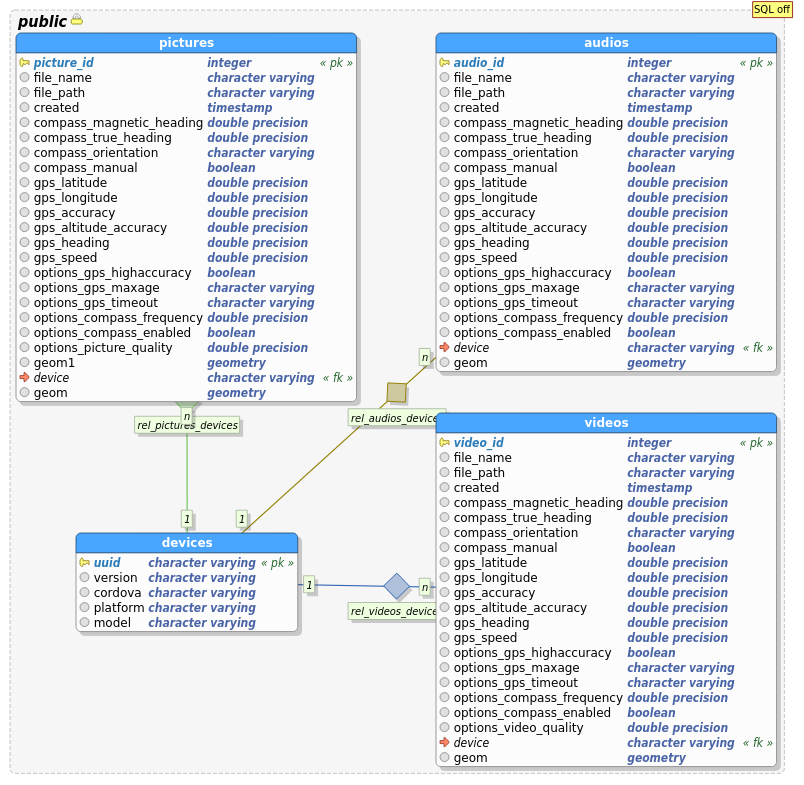
\includegraphics[width=0.7\textwidth]{figuras/moduledb.png}
\caption{Disposi��o das tabelas de banco de dados utilizada neste m�dulo.}
\label{fig:moduledb}
\end{figure}

Assim, o servi�o web desenvolvido utilizando Flask permite usar os principais m�todos do protocolo HTTP, atrav�s do estilo arquitetural REST, para tratar as solicita��es dos dados, conforme Tabela \ref{tab:rest_prototipo}.

\begin{table}[h]
\centering
\caption{Configura��o do Servidor REST do Projeto.}
\small
\label{tab:rest_prototipo}
\resizebox{\textwidth}{!}{%
\begin{tabular}{@{}lll@{}}
\toprule
M�todo HTTP & Descri��o da A��o                                                                       & Recurso                                                                                                                                                              \\ \midrule
GET         & \begin{tabular}[t]{@{}l@{}}Obter informa��es sobre\\ um ou v�rios recursos\end{tabular} & \begin{tabular}[t]{@{}l@{}}/api/\{recursos\}\\ (onde \{recursos\} pode ser \\ 'pictures', 'videos' ou 'audios')\end{tabular}                                         \\
GET         & \begin{tabular}[t]{@{}l@{}}Obter informa��es sobre\\ um ou v�rios recursos\end{tabular} & \begin{tabular}[t]{@{}l@{}}/api/\{recurso\}/\#id\\ (onde \{recurso\} pode ser \\ 'picture', 'video' ou 'audio'\\ e \#id � a identifica��o do\\ recurso)\end{tabular} \\
PUT         & \begin{tabular}[t]{@{}l@{}}Atualizar informa��es\\  de um recurso\end{tabular}          & \begin{tabular}[t]{@{}l@{}}/api/\{recurso\}/\#id\\ (onde \{recurso\} pode ser \\ 'picture', 'video' ou 'audio'\\ e \#id � a identifica��o do\\ recurso)\end{tabular} \\
DELETE      & \begin{tabular}[t]{@{}l@{}}Remover a informa��o\\  de um recurso\end{tabular}           & \begin{tabular}[t]{@{}l@{}}/api/\{recurso\}/\#id\\ (onde \{recurso\} pode ser \\ 'picture', 'video' ou 'audio'\\ e \#id � a identifica��o do\\ recurso)\end{tabular}
\end{tabular}
}
\end{table}

Um servi�o web REST permite envio de arquivos para o servidor de tr�s formas:
\begin{enumerate}
    \item Utiliza��o de Base64, onde o arquivo � codificado para uma \textit{strings} de 64 caracteres para ser enviado na requisi��o.
    \item \textit{multipart/form-data} e \textit{metadata}. Utilizar um formul�rio, \textit{FormData}\footnote{\url{https://developer.mozilla.org/en-US/docs/Web/Guide/Using_FormData_Objects}}, para enviar apenas os arquivos necess�rios e aguardar o retorno URI deste arquivo gerado e utilizar o m�todo \textit{PUT} para atualizar as informa��es deste.
    \item \textit{metadata} e \textit{multipart/form-data}. M�todo semelhante ao mencionado acima, por�m primeiro � enviado as informa��es do arquivo e um URI � aguardado, uma veste este retornado o arquivo � encaminhado com a identifica��o do URI.
\end{enumerate}

Apesar destas 3 formas estarem corretas tratando-se de uma arquitetura REST, elas apresentam algumas desvantagens. A primeira aumenta o tamanho do arquivo a ser trafegado pela rede, aumento que pode chegar a mais 33\% do tamanho original. A segunda e terceira esperam um retorno do servidor para continuar o envio, o que eleva a quantidade de transfer�ncias necess�rias.

Assim, optou-se que enviar um arquivo pelo m�todo tradicional, no contexto web, atrav�s de \textit{FormData}, onde arquivos e uma estrutura de chave e valores s�o informados. Esta estrutura de chave e valores tem que ser padronizada para que o servidor web que recebe a requisi��o possa saber quais as chaves est�o sendo enviadas e quais s�o necess�rias. Os valores de cada chave s�o os objetos JSON propriamente codificados.

Portanto, uma vez que uma requisi��o de envio de imagens foi feita ao servidor do projeto, espera-se um formul�rio \textit{multipart/form-data} com o arquivo utilizando \textit{FormData} e as informa��es atrav�s de chave e valores de um formul�rio padr�o\footnote{\url{https://developer.mozilla.org/en-US/docs/Web/API/XMLHttpRequest/Using_XMLHttpRequest\#Submitting_forms_and_uploading_files}}.

\subsubsection{Front-End} % (fold)
\label{ssub:front_end}

Para este projeto, uma p�gina web foi desenvolvida para que os dados captados pelos volunt�rios utilizando o aplicativo h�brido pudessem ser visualizados. Esta p�gina tem que cumprir alguns requisitos para melhor exibir os dados, a saber:

\begin{itemize}
    \item Visualizar de forma r�pida todos os dados dispon�veis;
    \item Visualizar as propriedades de um dado selecionado;
    \item Exibir o conte�do de um dado selecionado (imagem, �udio ou v�deo);
    \item Exibir os dados georreferenciados utilizando mapas ou imagens de sat�lite;
    \item Identificar os diferentes tipos de dados no mapa;
    \item Permitir que o usu�rio alterne o mapa em exibi��o;
\end{itemize}

Assim, ap�s alguns prot�tipos da interface da aplica��es web, foi desenvolvida uma p�gina web conforme ilustrado na Figura \ref{fig:frontend_mocqup}, que traz algumas das principais funcionalidades enumeradas abaixo:

\begin{enumerate}[label=\arabic*.]
    \item \textbf{Barra de Navega��o.} Reunindo as principais liga��es externas do s�tio, a barra de navega��o � uma importante ferramenta para os sistemas web. O usu�rio pode utilizar esta para conhecer outros recursos que o s�tio pode apresentar. Diversos tipos de recursos podem ser adicionados  a este componente, como menus, seletores, pesquisa e at� formul�rios. A barra de navega��o em quest�o deve permanecer sempre acima do mapa, para que os usu�rios possam navegar para outros links.

    \item \textbf{Mapa.} Um requisito de uma aplica��o web que utiliza dados georreferenciado � poder exibi-los em um mapa. O usu�rio pode utilizar o mapa para localizar-se melhor.

    \item \textbf{Seletor de Camadas.} Uma grande vantagem das aplica��es web com mapas � a possibilidade de exibir diversas camadas em uma �nica aplica��o. Pode ser exibida uma camada, aplicar transpar�ncia nesta e exibir outras diversas camadas deste modo, formando assim um grande mosaico de imagens georreferenciadas. Este tamb�m poder� permitir a altera��o da visibilidade dos dados captados, por exemplo, escondendo a camada de fotos, mas manter a de v�deo e �udio vis�veis.

    \item \textbf{�udio.} Representa��o de um dado de �udio que ao apertar um bot�o, este invoca uma janela modal mostrando todas as suas propriedades.
    \begin{enumerate}[label=4\alph*.]
        \item A miniatura de uma imagem representando um arquivo de �udio na navega��o que ao apertar um bot�o, este invoca uma janela modal mostrando todas as suas propriedades.
    \end{enumerate}

    \item \textbf{Foto.} Representa��o de um dado de foto que ao apertar um bot�o, este invoca uma janela modal mostrando todas as suas propriedades.
    \begin{enumerate}[label=5\alph*.]
        \item A miniatura de uma imagem representando um arquivo de foto na navega��o que ao apertar um bot�o, este invoca uma janela modal mostrando todas as suas propriedades.
    \end{enumerate}

    \item Uma miniatura de imagem representando um arquivo de �udio na navega��o que ao apertar um bot�o, este invoca uma janela modal mostrando todas as suas propriedades.
    \begin{enumerate}[label=6\alph*.]
        \item V�deo em navega��o.
        \item Janela de Propriedades do v�deo. O mesmo para outros tipos de m�dia.
        \item Exibi��o do conte�do do v�deo. O mesmo para outros tipos de m�dia.
        \item Propriedades do v�deo. O mesmo para outros tipos de m�dia.
    \end{enumerate}

    \item Navega��o. Utiliza miniaturas de imagens para facilitar a navega��o do volunt�rio a procurar uma determinada imagem. Cada vez que uma dessas miniaturas � selecionada, o seu ponto de refer�ncia no mapa � destacado e uma janela com suas propriedades pode ser visualizada.
\end{enumerate}

\begin{figure}[h]
\centering
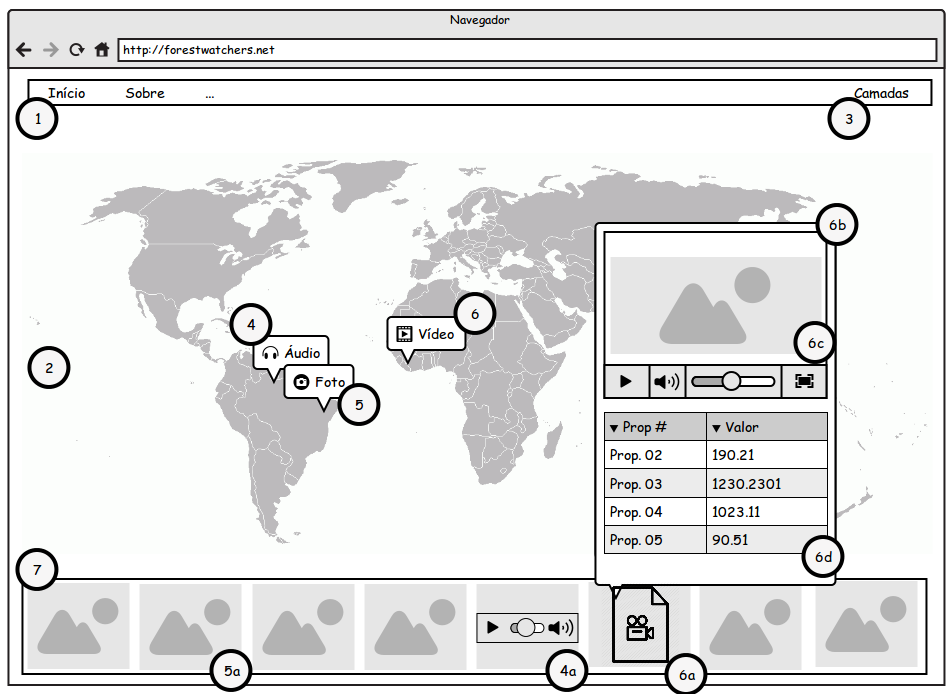
\includegraphics[width=0.6\textwidth]{figuras/frontend_mocqup.png}
\caption{Esbo�o da p�gina de visualiza��o dos resultados, destacando as principais fun��es conforme descrito acima.}
\label{fig:frontend_mocqup}
\end{figure}

Para o desenvolvimento desta p�gina foi utilizado os \textit{frameworks} Twitter Bootstrap, OpenLayers 2, jQuery e Sly. A Tabela \ref{tab:front_frameworks} descreve cada um destes frameworks.

\begin{table}[h]
\centering
\small
\caption{Componentes Utilizado na Interface Gr�fica.}
\label{tab:front_frameworks}

\begin{tabular}{| p{2.5cm} | p{12cm} |}
\hline
Framework            & Descri��o \\ \hline
Twitter Bootstrap   & O Twitter Bootstrap � um \textit{framework} para desenvolvimento de interface gr�fica permite novas cria��es de forma r�pida e simples. Conhecido por permitir um desenvolvimento r�pido para dispositivos m�veis, o Bootstrap, possui diversas funcionalidades que s�o acessados atrav�s da utiliza��o de JavaScript com CSS. Endere�o \url{http://getbootstrap.com} \\ \hline
OpenLayers2         & Um dos primeiros e mais utilizados \textit{frameworks} para exibi��o de dados geogr�ficos, o OpenLayers, possui diversas funcionalidades para mostrar gr�ficos em uma p�gina HTML. Endere�o\url{http://openlayers.org/two} \\ \hline
jQuery                   & Diversas funcionalidades do JavaScript s�o encapsuladas atrav�s deste framework tornando o desenvolvimento de p�ginas din�micas mais simples. O jQuery permite fazer chamadas XMLHttpRequest (XHR) de forma f�cil, essas chamadas caracter�sticas de p�ginas din�micas, permitem carregar conte�dos de servidores remotos e atualizar a p�gina em exibi��o. Endere�o \url{http://jquery.com} \\ \hline
Sly                        & Sly, este � um framework para a exibi��o de imagens em miniaturas onde o usu�rio pode, com o mouse ou com o movimento das m�os, mover as imagens de forma din�mica. Endere�o \url{http://darsa.in/sly} \\ \hline
MapServer            & O MapServer � um servidor de mapas que permite distribuir dados espaciais de forma que estes possam ser renderizados por outros servi�os, seguindo padr�es geogr�ficos como GML, GeoJSON e outros.  Endere�o \url{http://mapserver.org} \\ \hline
\end{tabular}
\end{table}

\pagebreak

Quando a p�gina � exibida, as camadas encontradas dispon�veis no servidor local MapServer s�o carregados. Estas camadas podem ser de um arquivo de Imagem (raster) ou uma camada de pontos (vetorial), o usu�rio poder� optar por visualizar cada uma destas camadas. Os arquivos de foto, v�deo e �udio que foram foram enviados pelos volunt�rios s�o exibidos no s�tio, permitindo que o usu�rio possa interagir com estes. A Figura \ref{fig:UMLFrontEndSequence} ilustra este processo.

\begin{figure}[h]
\centering
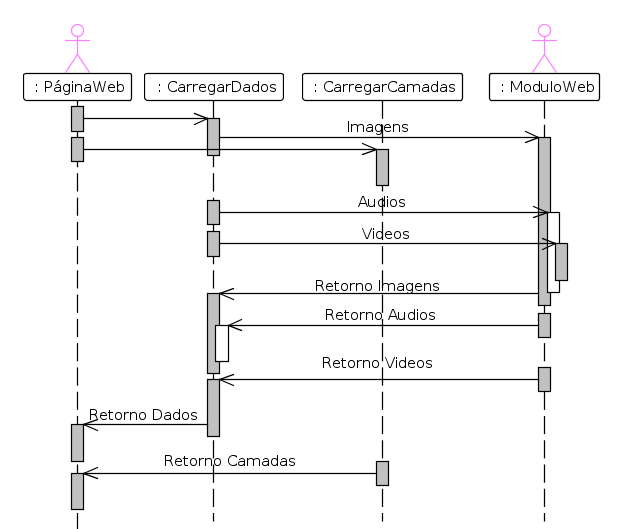
\includegraphics[width=0.6\textwidth]{figuras/UML/UMLFrontEndSequence.png}
\caption{UML de Sequ�ncia do processo de carregamento das camadas, imagens, �udios e v�deos necess�rias para o funcionamento da p�gina web do m�dulo se sensoriamento volunt�rio.}
\label{fig:UMLFrontEndSequence}
\end{figure}

\pagebreak

Por fim, a Tabela \ref{tab:sumarizacao} faz um breve resumo dos componentes utilizados no desenvolvimento deste projeto descritos nesta se��o. Apesar de haver diversos outros componentes com funcionalidades semelhantes a alguns dos componentes selecionados, estes n�o foram considerados neste trabalho devido � prefer�ncia por manter a compatibilidade com outros componentes j� em utiliza��o pelo projeto ForestWatchers, como PostgreSQL e MapServer.

\begin{table}[h]
\centering
\caption{Sumariza��o dos componentes utilizados.}
\label{tab:sumarizacao}
\resizebox{\textwidth}{!}{%
\begin{tabular}{|c|l|c|l|}
\hline
\begin{tabular}[c]{@{}c@{}}Subsistema \\ ou Aplicativo \\ ou Componente\end{tabular}           & \multicolumn{1}{c|}{\begin{tabular}[c]{@{}c@{}}Solu��es \\ ou Tecnologias Dispon�veis \\ ou Testadas\end{tabular}} & \begin{tabular}[c]{@{}c@{}}Solu��o \\ Adotada\end{tabular} & \multicolumn{1}{c|}{Motivo}                                                                                                                                                                                  \\ \hline
\multirow{8}{*}{\begin{tabular}[c]{@{}c@{}}Aplicativo \\ para \\ Coleta de Dados\end{tabular}} & Aplicativo de Sistema Pronto:                                                                                      & \multicolumn{1}{l|}{}                                      &                                                                                                                                                                                                              \\
                                                                                               & EpiCollect                                                                                                         & \multicolumn{1}{l|}{}                                      &                                                                                                                                                                                                              \\
                                                                                               & EpiCollect+                                                                                                        & \multicolumn{1}{l|}{}                                      &                                                                                                                                                                                                              \\
                                                                                               & Sensr                                                                                                              & \multicolumn{1}{l|}{}                                      &                                                                                                                                                                                                              \\ \cline{2-4}
                                                                                               & Aplicativo Nativo:                                                                                                 & \multicolumn{1}{l|}{}                                      &                                                                                                                                                                                                              \\
                                                                                               & Desenvolvido para Windows Phone                                                                                    & \multicolumn{1}{l|}{}                                      &                                                                                                                                                                                                              \\ \cline{2-4}
                                                                                               & Aplicativo H�brido:                                                                                                & \multicolumn{1}{l|}{}                                      &                                                                                                                                                                                                              \\
                                                                                               & \begin{tabular}[c]{@{}l@{}}Desenvolvido com PhoneGap,\\ jQueryMobile, KnockoutJS \end{tabular}                     & X                                                          & \begin{tabular}[c]{@{}l@{}}Desenvolvimento baseado em \\ Web (HTML5, CSS, JavaScript) \\ e dispon�vel para um grande \\ n�mero de plataformas.\end{tabular}                                                  \\ \hline
\multirow{9}{*}{\begin{tabular}[c]{@{}c@{}}Servidor \\ para \\ Internet\end{tabular}}          & Back-End:                                                                                                          &                                                            &                                                                                                                                                                                                              \\
                                                                                               & PostgreSQL                                                                                                         & X                                                          & \begin{tabular}[c]{@{}l@{}}Banco de dados escolhido por\\ ser parte integrante do componente\\ PyBossa, assim n�o tendo necessidade\\ de instalar diferentes softwares com\\ o mesmo prop�sito.\end{tabular} \\ \cline{2-4}
                                                                                               & Flask                                                                                                              & X                                                          & \begin{tabular}[c]{@{}l@{}}Servidor Web escolhido por\\ ser parte integrante do componente\\ PyBossa, assim n�o tendo necessidade\\ de instalar diferentes softwares com\\ o mesmo prop�sito.\end{tabular}   \\ \cline{2-4}
                                                                                               & Front-End:                                                                                                         &                                                            &                                                                                                                                                                                                              \\
                                                                                               & Twitter Bootstrap                                                                                                  & X                                                          & \begin{tabular}[c]{@{}l@{}}Oferece facilidade para o desenvolvimento\\ HTML5\end{tabular}                                                                                                                    \\ \cline{2-4}
                                                                                               & OpenLayers2                                                                                                        & X                                                          & \begin{tabular}[c]{@{}l@{}}Gerenciamento de mapas para ambiente\\ Web\end{tabular}                                                                                                                           \\ \cline{2-4}
                                                                                               & Jquery                                                                                                             & X                                                          & \begin{tabular}[c]{@{}l@{}}Facilitador para manusear scripts feitos\\ em JavaScript\end{tabular}                                                                                                             \\ \cline{2-4}
                                                                                               & Sly                                                                                                                & X                                                          & \begin{tabular}[c]{@{}l@{}}Permite criar miniaturas de imagens ou\\ elementos HTML\end{tabular}                                                                                                              \\ \cline{2-4}
                                                                                               & MapServer                                                                                                          & X                                                          & \begin{tabular}[c]{@{}l@{}}Respons�vel por renderizar imagens para\\ mapas em ambiente Web\end{tabular}                                                                                                      \\ \hline
\end{tabular}
}
\end{table}





\chapter{TESTE DO M�DULO DE SV}
\label{ch:resultados}

A �rea utilizada para testar o m�dulo de SV desenvolvido nesta disserta��o (Figura \ref{fig:para_exported}) faz parte da Floresta dos Tapaj�s, uma reserva federal, e seus arredores. Localizado na cidade de Belterra, PA, dentro portanto da Amaz�nia Legal. Esta � uma regi�o de floresta tropical. O processo de ocupa��o na regi�o ocorreu ao longo da rodovia BR-163, depois do desmatamento da floresta prim�ria e abertura de novas estradas para a forma��o de pequenas fazendas. Como resultado deste processo, existem mosaicos de vegeta��es secund�rias em diversos est�gios de desenvolvimento. �reas de  pasto, milharais e solos expostos dentro de florestas \cite{LongoReDeBeRiMe:2012:PhChPa}.

A visita a esta �rea s� foi poss�vel por uma oportunidade oferecida pelo Departamento de Processamento de Imagem (DPI) do INPE, que precisavam georreferenciar alguns pontos de interesse (POI) com alta precis�o e coletar alguns dados sobre a �rea, como exemplo o tipo de vegeta��o existente em um determinado local. Assim, alguns alunos de mestrado e doutorado puderam se beneficiar com uma viagem para validar seus estudos, em contrapartida poderiam auxiliar na capturas de novos POI e coletar dados da �rea. Para a captura das informa��es das �reas para o DPI do INPE, eram utilizadas formul�rios impressos, classificando os aspectos do local. Utilizando-se de uma c�mera fotogr�fica com GPS interno, imagens georreferenciadas eram capturadas e anotadas junto ao formul�rio, uma b�ssola tamb�m era utilizada para capturar o sentido em que a foto fora capturada e sua informa��o escrita no formul�rio.

Para o teste do conceito desenvolvido neste trabalho, utilizou-se o aplicativo h�brido (ver Se��o \ref{ssub:aplicativo_com_biblioteca_hibrida}) na �rea de estudo para captar imagens, v�deos e �udios de algum interesse ao projeto FW, como �reas n�o florestas, clareiras, fazendas ou fauna. �reas de clareiras, por exemplo, podem apresentar diferentes formas em uma imagem de sat�lite de baixa resolu��o espacial tipo MODIS, sendo muitas vezes impercept�vel do espa�o. Com as fotos obtidas em \textit{in-situ} pelos volunt�rios � poss�vel complementar e mesmo corrigir os mapas de desmatamento gerados pelos volunt�rios que apenas t�m acesso a imagens de sat�lite.

\begin{figure}[h]
\centering
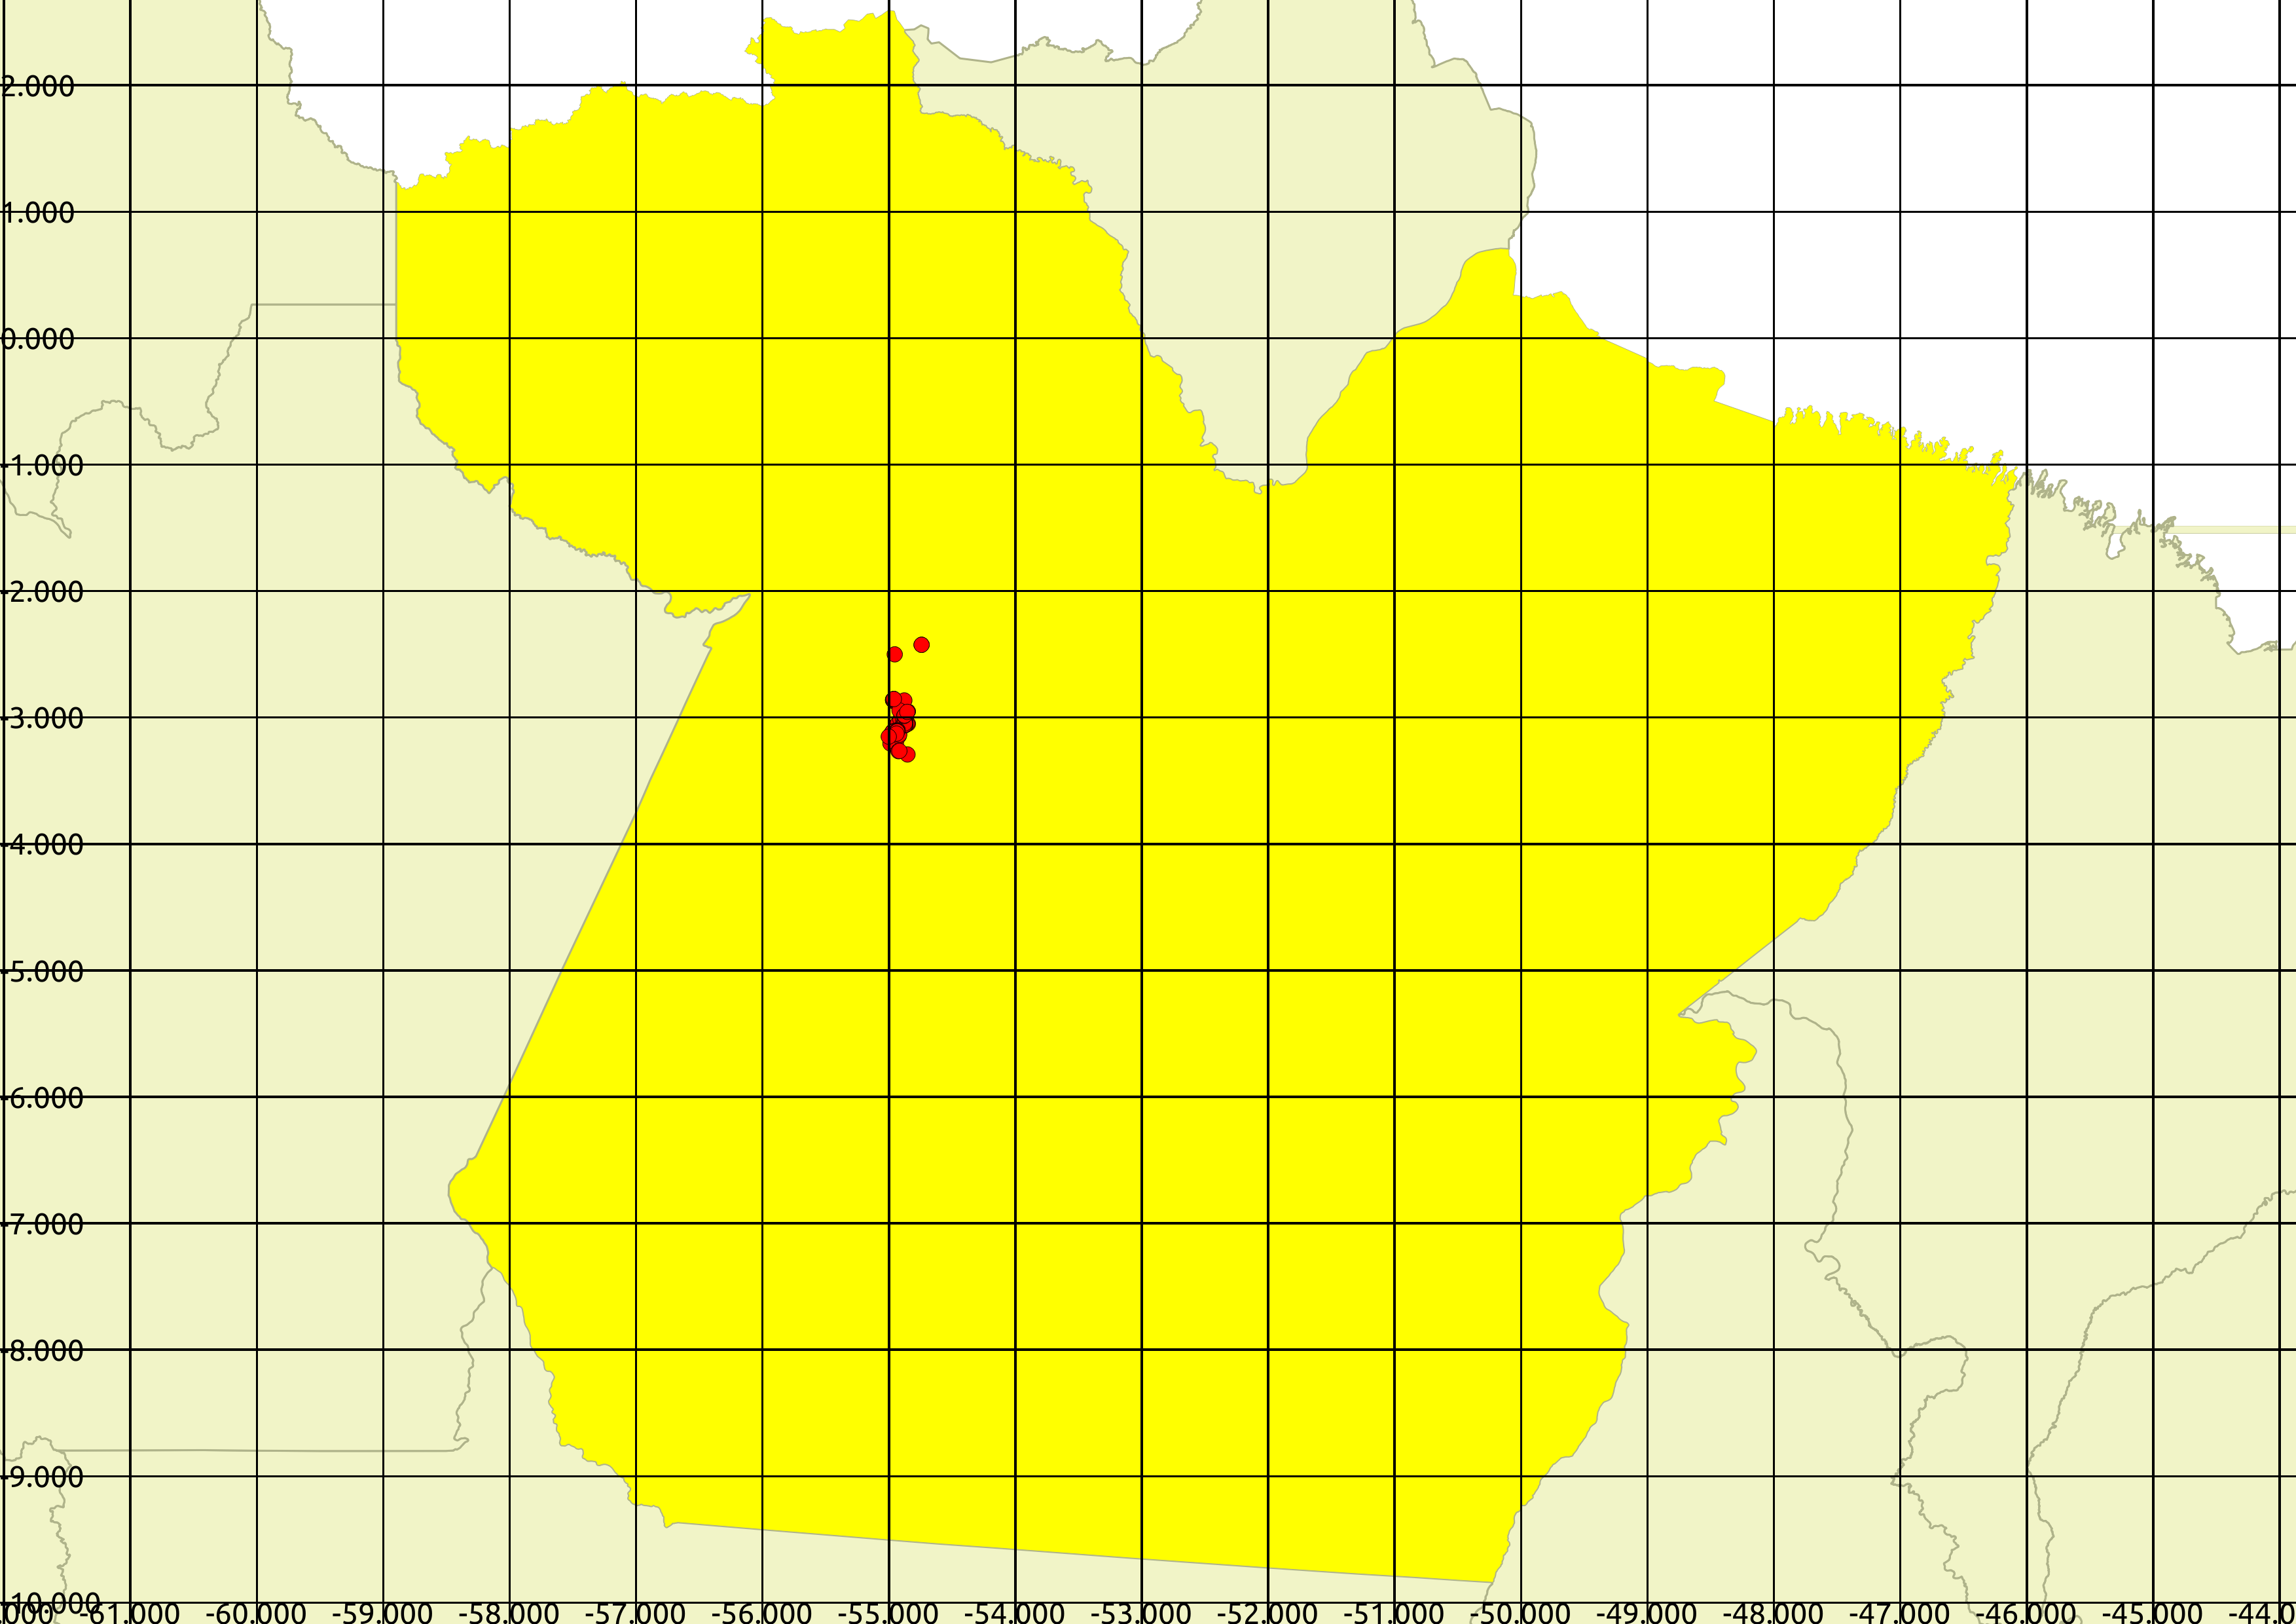
\includegraphics[width=0.9\textwidth]{figuras/para_exported.png}
\caption{�rea de interesse.}
\label{fig:para_exported}
\end{figure}

Durante a fase de testes, utilizou-se um dispositivo m�vel Lumia 800, um \textit{smartphone} com o sistema operacional Windows Phone, GPS e b�ssola interna. Para assegurar a qualidade dos dados georreferenciados coletados, foi utilizado em conjunto com o dispositivo m�vel uma b�ssola magn�tica e tamb�m um aparelho Garmin GPSMAP 60CSx\footnote{\url{https://buy.garmin.com/en-US/US/on-the-trail/discontinued/gpsmap-60csx/prod310.html}}.

Durante os 15 dias de experimento em campo, foram feitas 93 capturas com o aplicativo, sendo 83 imagens e 10 v�deos. N�o foi poss�vel efetuar captura de �udio devido a um erro no c�digo na biblioteca h�brida PhoneGap na vers�o 2.9. Neste caso, para testar o \textit{front-end} do m�dulo, foram utilizados �udios extra�dos dos v�deos.

Todos os dados foram capturados e mantidos no aparelho para que pudessem ser sincronizados posteriormente.

A Figura \ref{fig:mapa_fullscreen} ilustra a interface desenvolvida neste trabalho para exibir os dados coletados, semelhante ao esbo�o visto na Figura \ref{fig:frontend_mocqup}. A interface cont�m as miniaturas das imagens e v�deos na parte inferior da tela, permitindo uma r�pida sele��o baseado no interesse do volunt�rio. Ao clicar em uma imagem ou v�deo, tanto nas miniaturas quanto nos �cones mostrados no mapa, uma pequena janela � exibida com as propriedades de destaque (canto inferior direito da Figura \ref{fig:mapa_fullscreen}).

\begin{figure}[h]
\centering
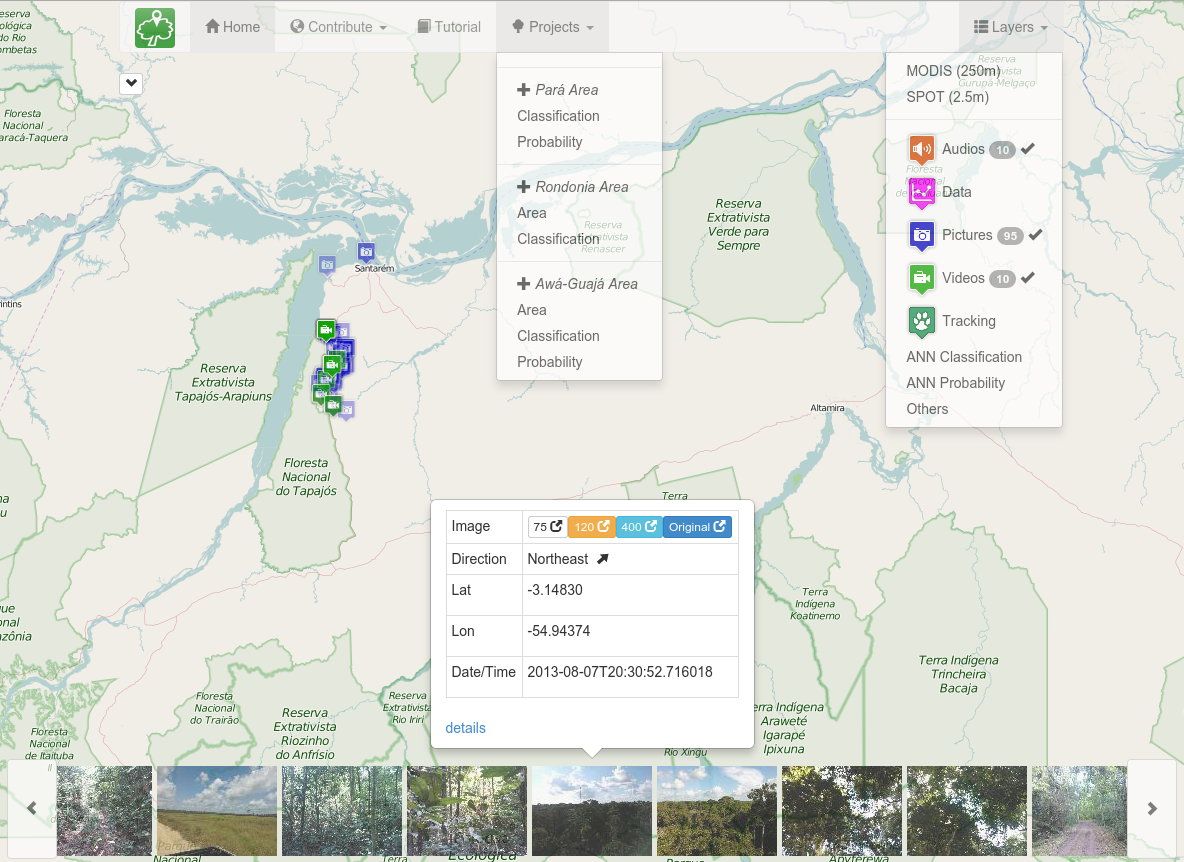
\includegraphics[width=0.9\textwidth]{figuras/resultados/full_map_with_menus.png}
\caption{Interface gr�fica \textit{(front-end)} desenvolvido para a exibi��o dos dados coletados pelos volunt�rios.}
\label{fig:mapa_fullscreen}
\end{figure}

Esta pequena janela � comum para os demais recursos (�udios, v�deos e imagens), por�m a primeira linha apresenta um aspecto diferente, conforme o tipo de dado selecionado. Caso venha ser uma imagem, s�o exibidos as diferentes dimens�es desta imagem, caso seja um �udio ou v�deo, uma janela � exibida com o respectivo conte�do pronto para reprodu��o (veja Fig. \ref{fig:detalhes_conteudos}).
\begin{figure}%
\centering
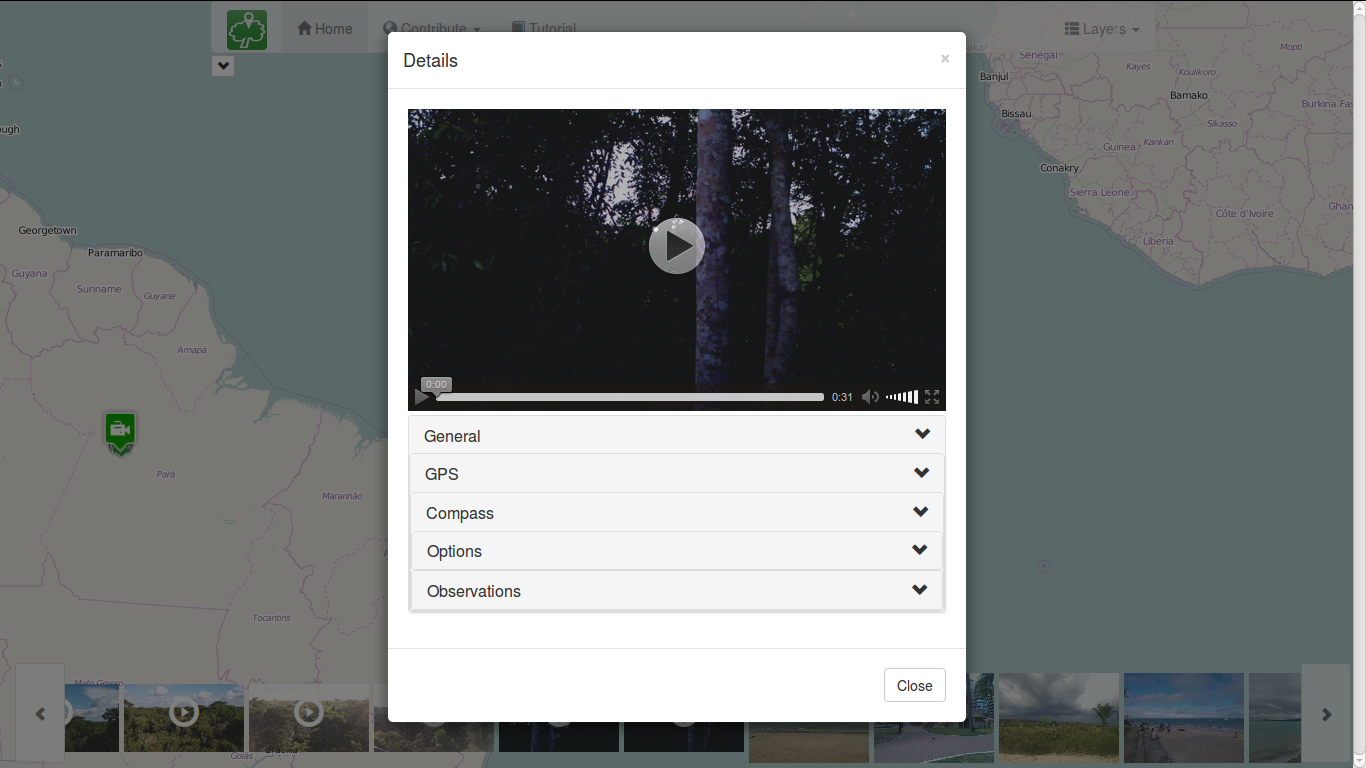
\includegraphics[width=0.495\textwidth]{figuras/resultados/detalhe_video.png}
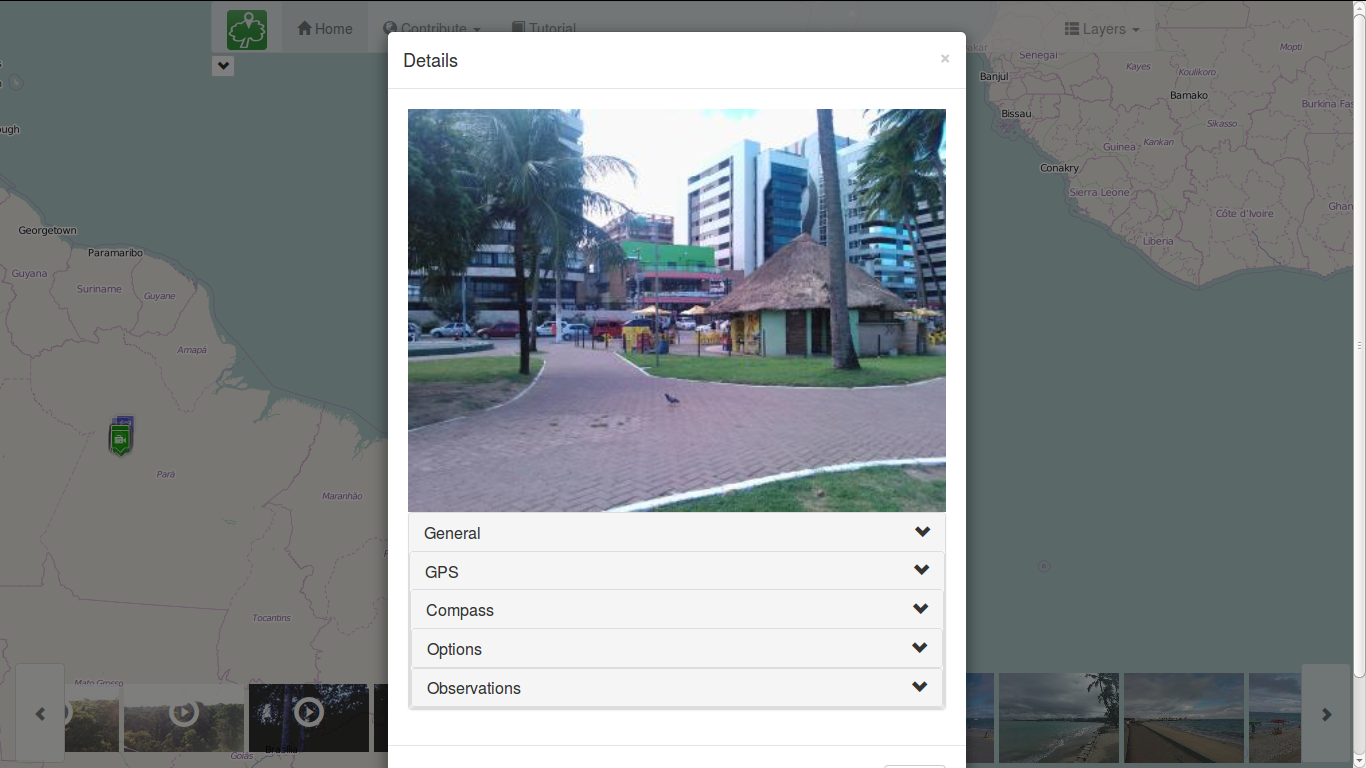
\includegraphics[width=0.495\textwidth]{figuras/resultados/detalhe_foto.png}
\qquad
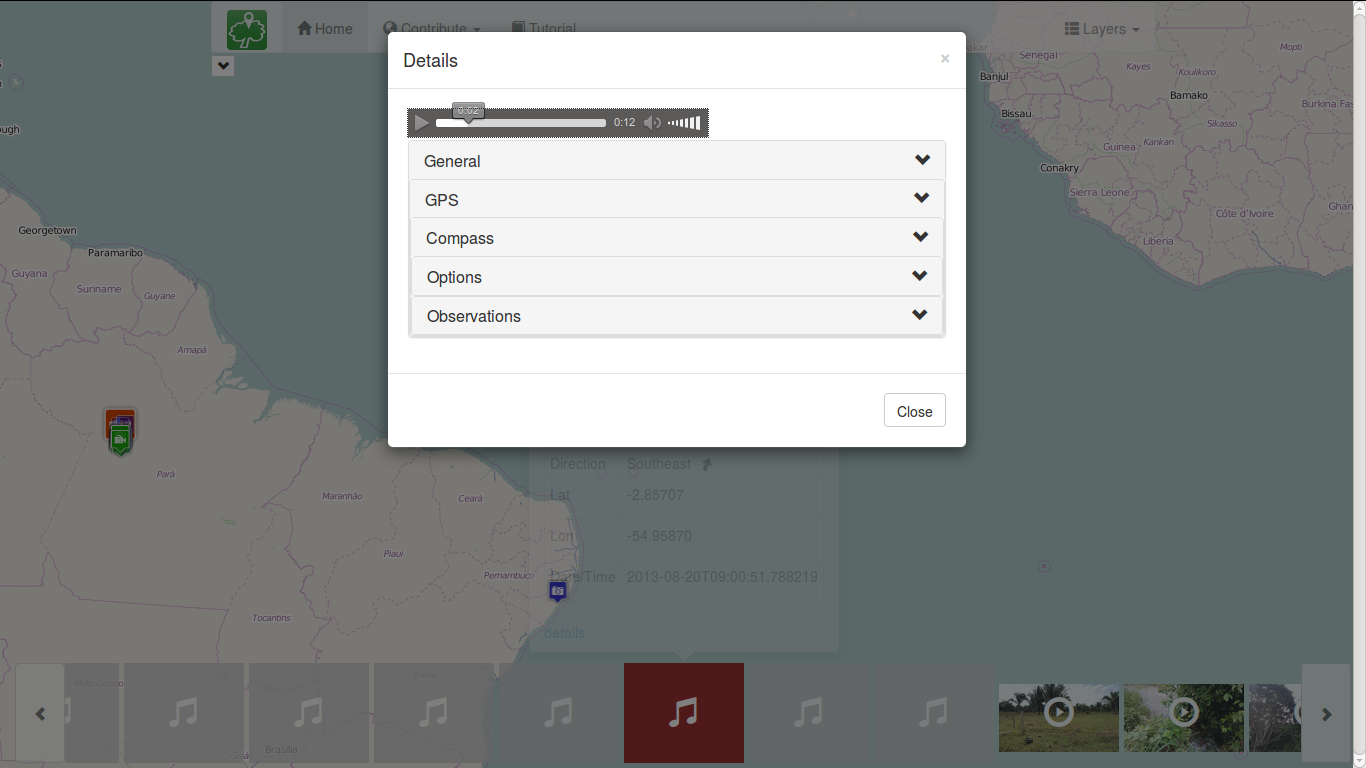
\includegraphics[width=0.495\textwidth]{figuras/resultados/detalhe_audio.png}
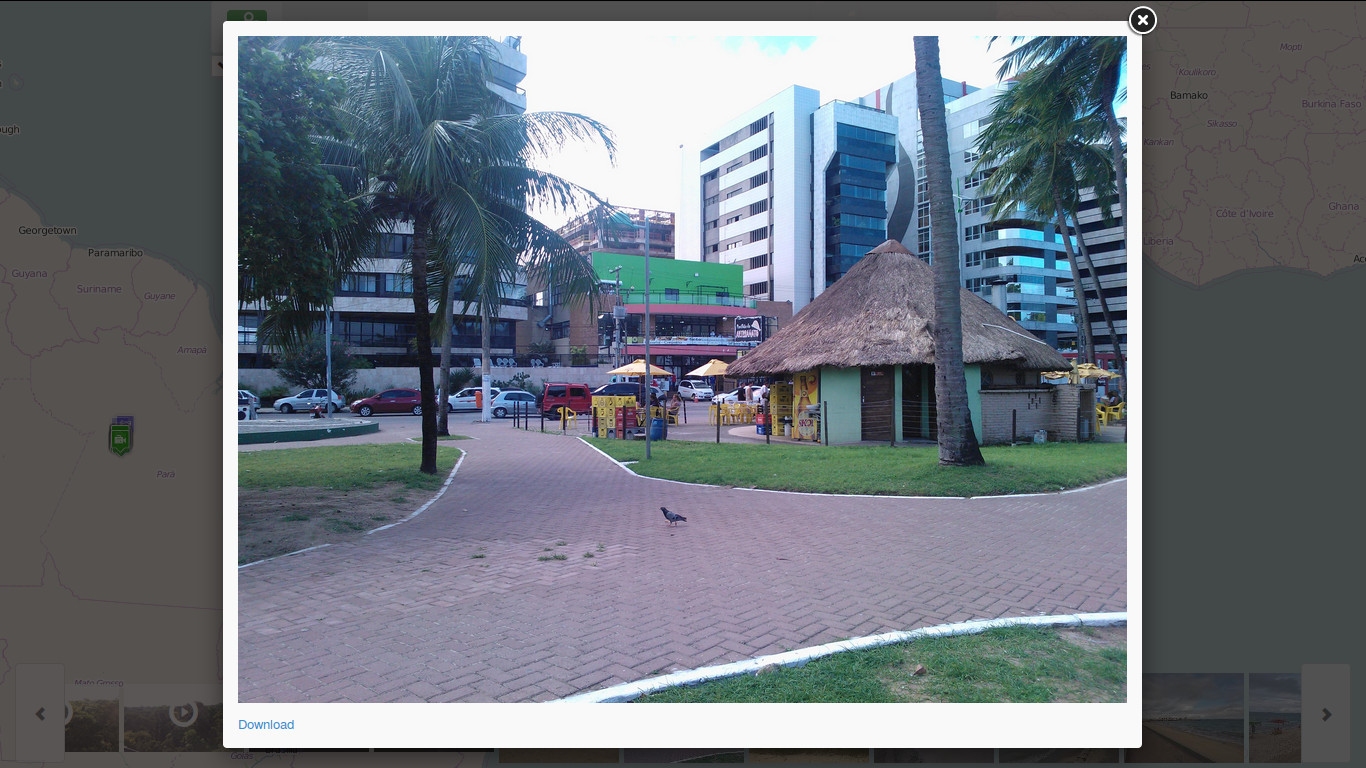
\includegraphics[width=0.495\textwidth]{figuras/resultados/selecao_imagem_foto.png}
\caption{No canto superior esquerdo, uma amostra de um v�deo capturado e pronto para exibi��o. No canto inferior esquerdo, uma grava��o de �udio pronto para ser reproduzida. Na esquerda, o detalhe de exibi��o de uma foto e a sele��o da imagem com melhor resolu��o, respectivamente na parte superior e inferior }%
\label{fig:detalhes_conteudos}%
\end{figure}

O mapa de fundo da Figura \ref{fig:mapa_fullscreen} � oferecido gratuitamente pelo projeto OpenStreetMaps, comentado na Se��o \ref{ch:informacao_geografica_voluntariada}. Por�m, a interface permite alternar a exibi��o dos mapas de fundo atrav�s da sele��o de camadas definidas no menu de ``Camadas'', no canto superior direito da tela (Canto superior direito da Figura \ref{fig:mapa_fullscreen}). Para este projeto foram definidas algumas camadas para melhor compreender este estudo; estas s�o:

\begin{itemize}
    \item \textbf{MODIS (250m).} A imagem MODIS selecionada faz parte do acervo de cat�logos de imagens r�pidas da NASA, FAS Brazil 7, imagem TERRA 2013216\footnote{\url{http://rapidfire.sci.gsfc.nasa.gov/imagery/subsets/?subset=FAS_Brazil7.2013216.terra.250m}} datado de 04 de Agosto de 2013, semana em que iniciou-se o estudo. Imagens MODIS foram comentadas na Se��o \ref{ch:monitoramento_florestas}.
    \item \textbf{SPOT (2.5m).} A imagem SPOT\footnote{\url{http://www.sema.pa.gov.br/2010/02/09/8665/}} possui resolu��o geogr�fica de 2.5 metros. Estas imagens, datadas de 11 de Julho de 2009 e 30 de Julho de 2011, s�o produtos comprados e processados pela Secretaria de Meio Ambiente (SEMA) do Estado do Par�, s�o utilizadas para uso acad�mico e est�o sendo usadas neste trabalho apenas para realizar compara��es com a imagem MODIS do mesmo local, por�m com resolu��o 10.000 vezes maior.
    \item \textbf{�udios.} Camada de pontos de �udio com suas propriedades.
    \item \textbf{Imagens.} Camada de pontos das imagens com suas propriedades, todas captadas utilizando o aplicativo h�brido.
    \item \textbf{V�deos.} Camada de pontos dos v�deos com suas propriedades, todas captadas utilizando o aplicativo h�brido.
    \item \textbf{Dados.} Camada de dados captados de sensores externos. Futuramente, ser� incorporado ao projeto.
    \item \textbf{Rastreio.} Camada de pontos provindos de rastreio. Futuramente, ser� incorporado ao projeto.
    \item \textbf{Classifica��o (RNA).} Imagem gerado pela classifica��o n�o supervisionada de uma rede neural artificial a partir da mesma imagem MODIS selecionada.
    \item \textbf{Probabilidade (RNA).} Imagem em escala de cinza da probabilidade de classifica��o da rede neural artificial ao classificar a imagem MODIS selecionada.
    \item \textbf{Outros.} Esta � uma camada agregada de tr�s outros mapas do Brasil: mapa hidrogr�fico, unidades de conserva��o e terras ind�genas.
    % imagens do dropbox do Eduardo, acredito que esteja no ForestWatchers.
\end{itemize}

Alternando as camadas, � poss�vel verificar mais precisamente a signific�ncia do pixel em quest�o. Uma imagem SPOT tem uma melhor clareza devido a sua resolu��o ser 10.000 vezes maior do que uma MODIS, o que permite verificar mais cuidadosamente o que h� na composi��o de um pixel MODIS.

Na Figura \ref{map:crop_map_modis} � poss�vel observar grandes �reas sem florestas, sendo estas os conjuntos de pixeis de tom mais claro. Contudo, n�o � trivial diferenciar um �nico pixel de uma imagem MODIS para identificar se este representa uma �rea florestada ou n�o.

\begin{figure}[h]
\centering
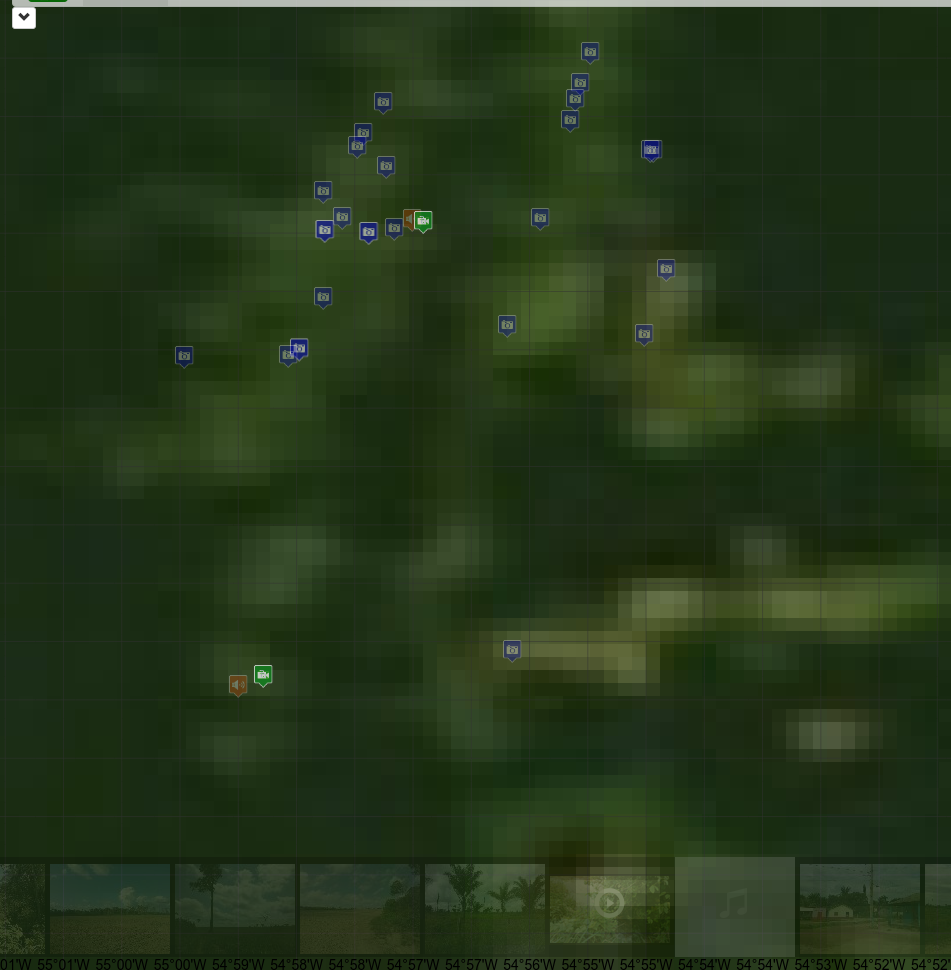
\includegraphics[width=\textwidth]{figuras/resultados/crop_map_modis.png}
\caption{Interface do m�dulo vista com a camada MODIS ativa.}
\label{map:crop_map_modis}
\end{figure}


A mesma �rea � apresentada na Figura \ref{map:crop_map_spot}. Esta camada torna a tarefa de diferenciar um pixel mais f�cil, bastando comparar a camada de imagem MODIS com a camada de imagem SPOT, uma vez que esta possui melhor resolu��o espacial.

\begin{figure}[h]
\centering
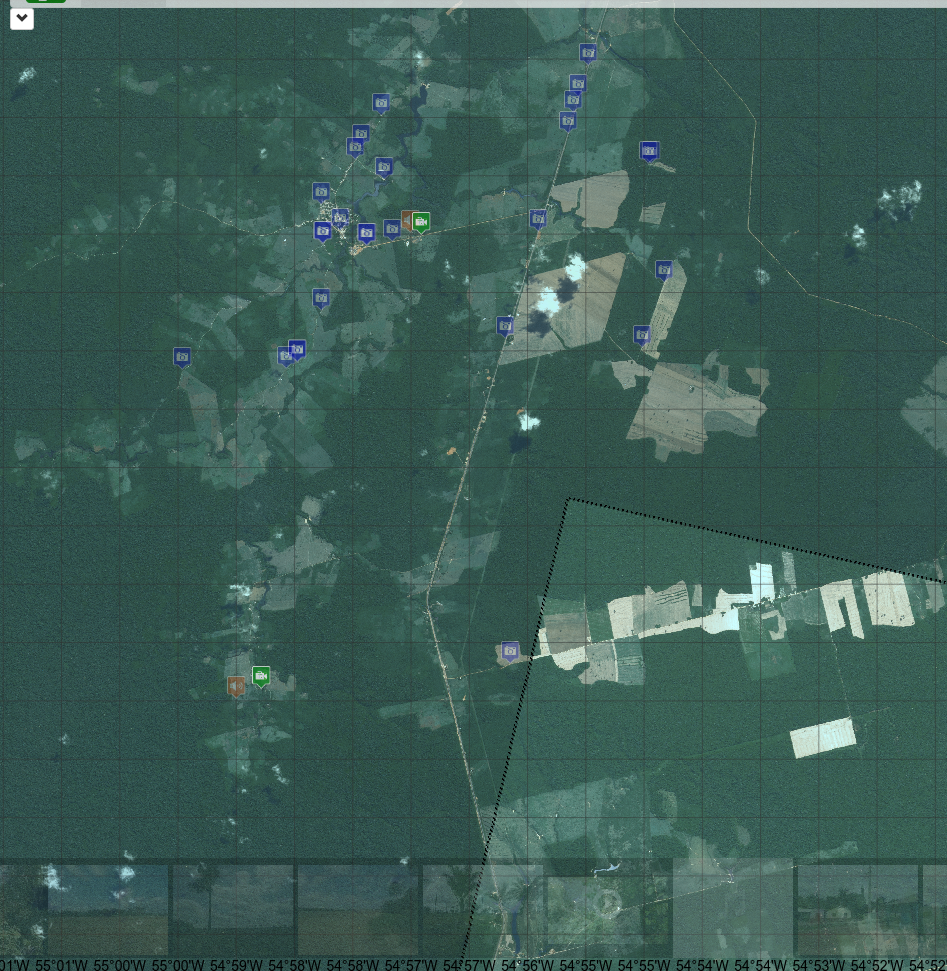
\includegraphics[width=\textwidth]{figuras/resultados/crop_map_spot.png}
\caption{Interface do m�dulo vista com a camada SPOT ativa.}
\label{map:crop_map_spot}
\end{figure}

Por�m, utilizar imagens SPOT, como � o caso deste trabalho, para comparar dois tipos de imagens em diferentes camadas n�o � vi�vel. Imagens SPOT s�o pagas, diferente das imagens MODIS. Al�m do mais, possuem um tempo de revisita diferente (em geral menor). Portanto, imagens, v�deos ou �udios captados \textit{in-situ} mant�m sua import�ncia na tarefa de discernir uma �rea florestada de uma �rea n�o-florestada.

A Figura \ref{map:small_map_modis} mostra a �rea compreendida pelas coordenadas 54\textdegree55'26.4''W a 03\textdegree07'33''S a 03\textdegree07'04.8''S de uma imagem MODIS. H� uma varia��o de cor no pixel que est� abaixo dos dois pontos de imagem. por�m � dif�cil saber ao certo se este representa uma �rea florestada ou n�o. Assim, as imagens \textit{in-situ} adquiridas pelo dispositivo podem dar uma contribui��o an�loga � camada SPOT.

\begin{figure}[h]
\centering
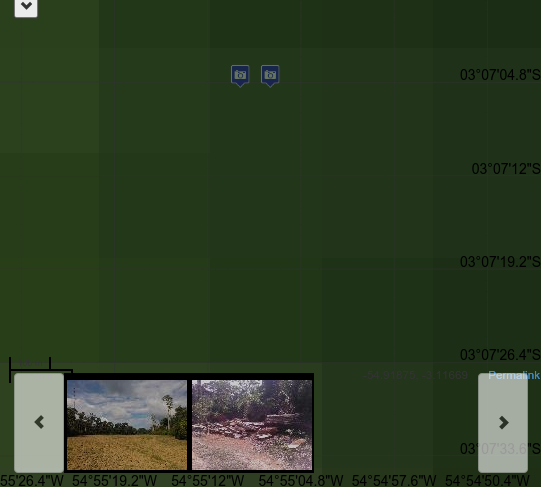
\includegraphics[width=\textwidth]{figuras/resultados/small_map_modis.png}
\caption{Dois pontos de imagem visualizados no mapa com a camada MODIS ativa.}
\label{map:small_map_modis}
\end{figure}

Na Figura \ref{map:small_selected_modis_left} � poss�vel observar o ponto da imagem no mapa com a camada MODIS selecionada e as propriedades deste ponto. Na direita da figura, a imagem capturada pelo aplicativo.

\begin{figure}[h]
\centering
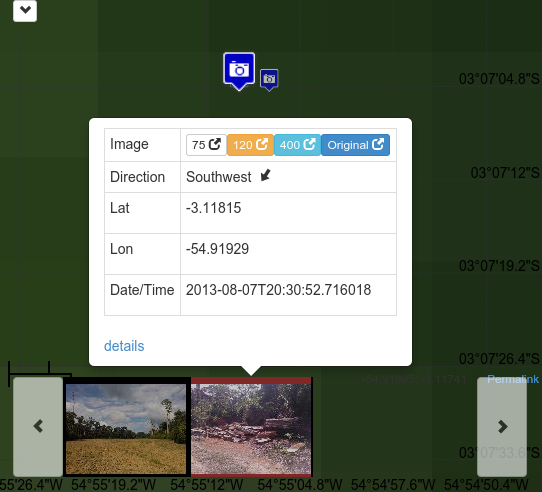
\includegraphics[width=0.495\textwidth]{figuras/resultados/small_selected_modis_left.png}
\hfill
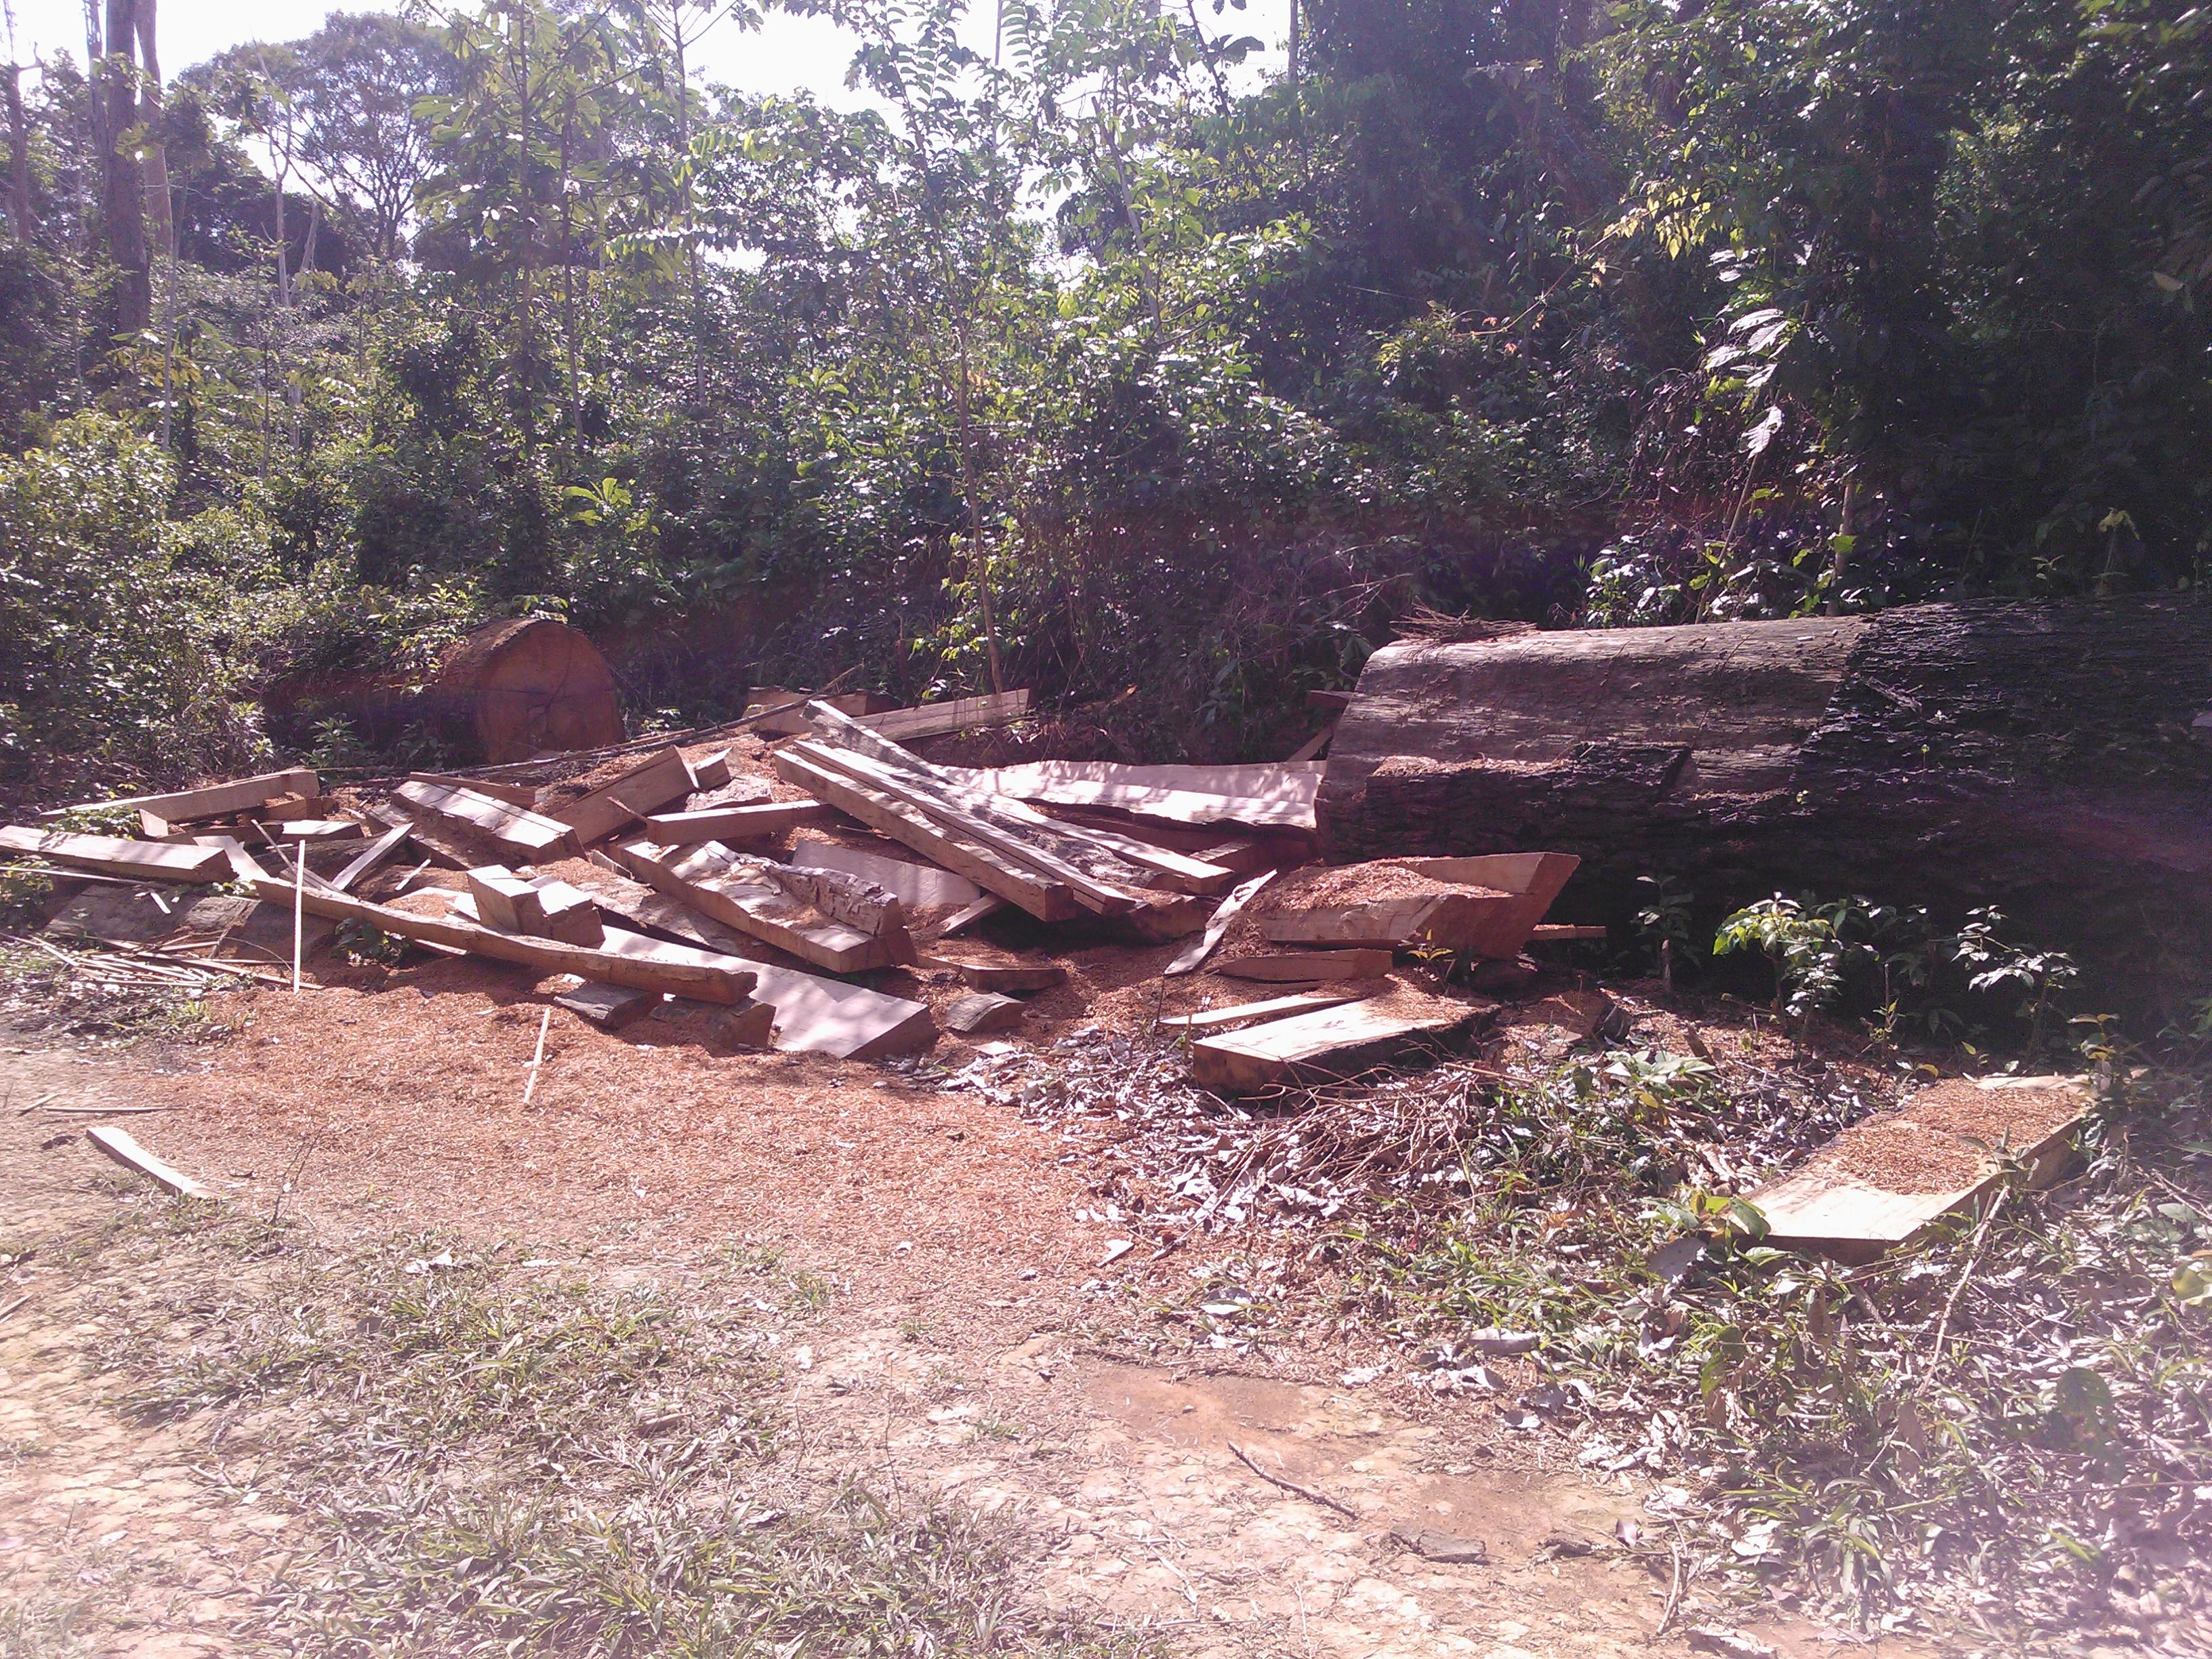
\includegraphics[width=0.495\textwidth]{figuras/resultados/small_modis_left.png}
\caption{Imagem de desmatamento. � esquerda, uma imagem selecionada e uma pequena janela com suas propriedades. � direita imagem capturada exibida em maior resolu��o. No mapa, uma camada MODIS ativa.}
\label{map:small_selected_modis_left}
\end{figure}

Outra imagem pode tamb�m ilustrar a situa��o nesta �rea. A Figura \ref{map:small_selected_modis_right} traz respectivamente da esquerda para a direita, uma imagem captada pelo aplicativo com suas propriedades e uma imagem de maior resolu��o para melhor visualiza��o.

\begin{figure}[h]
\centering
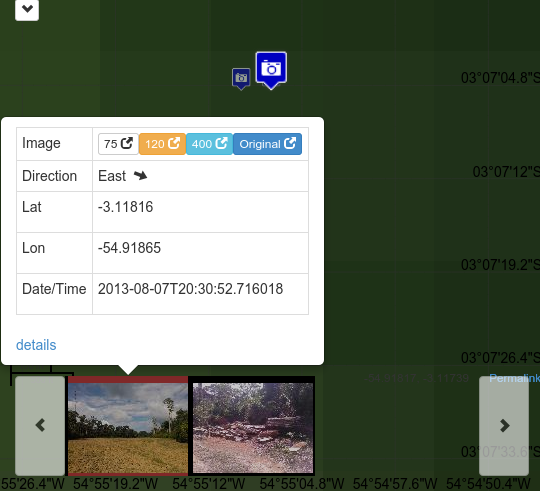
\includegraphics[width=0.495\textwidth]{figuras/resultados/small_selected_modis_right.png}
\hfill
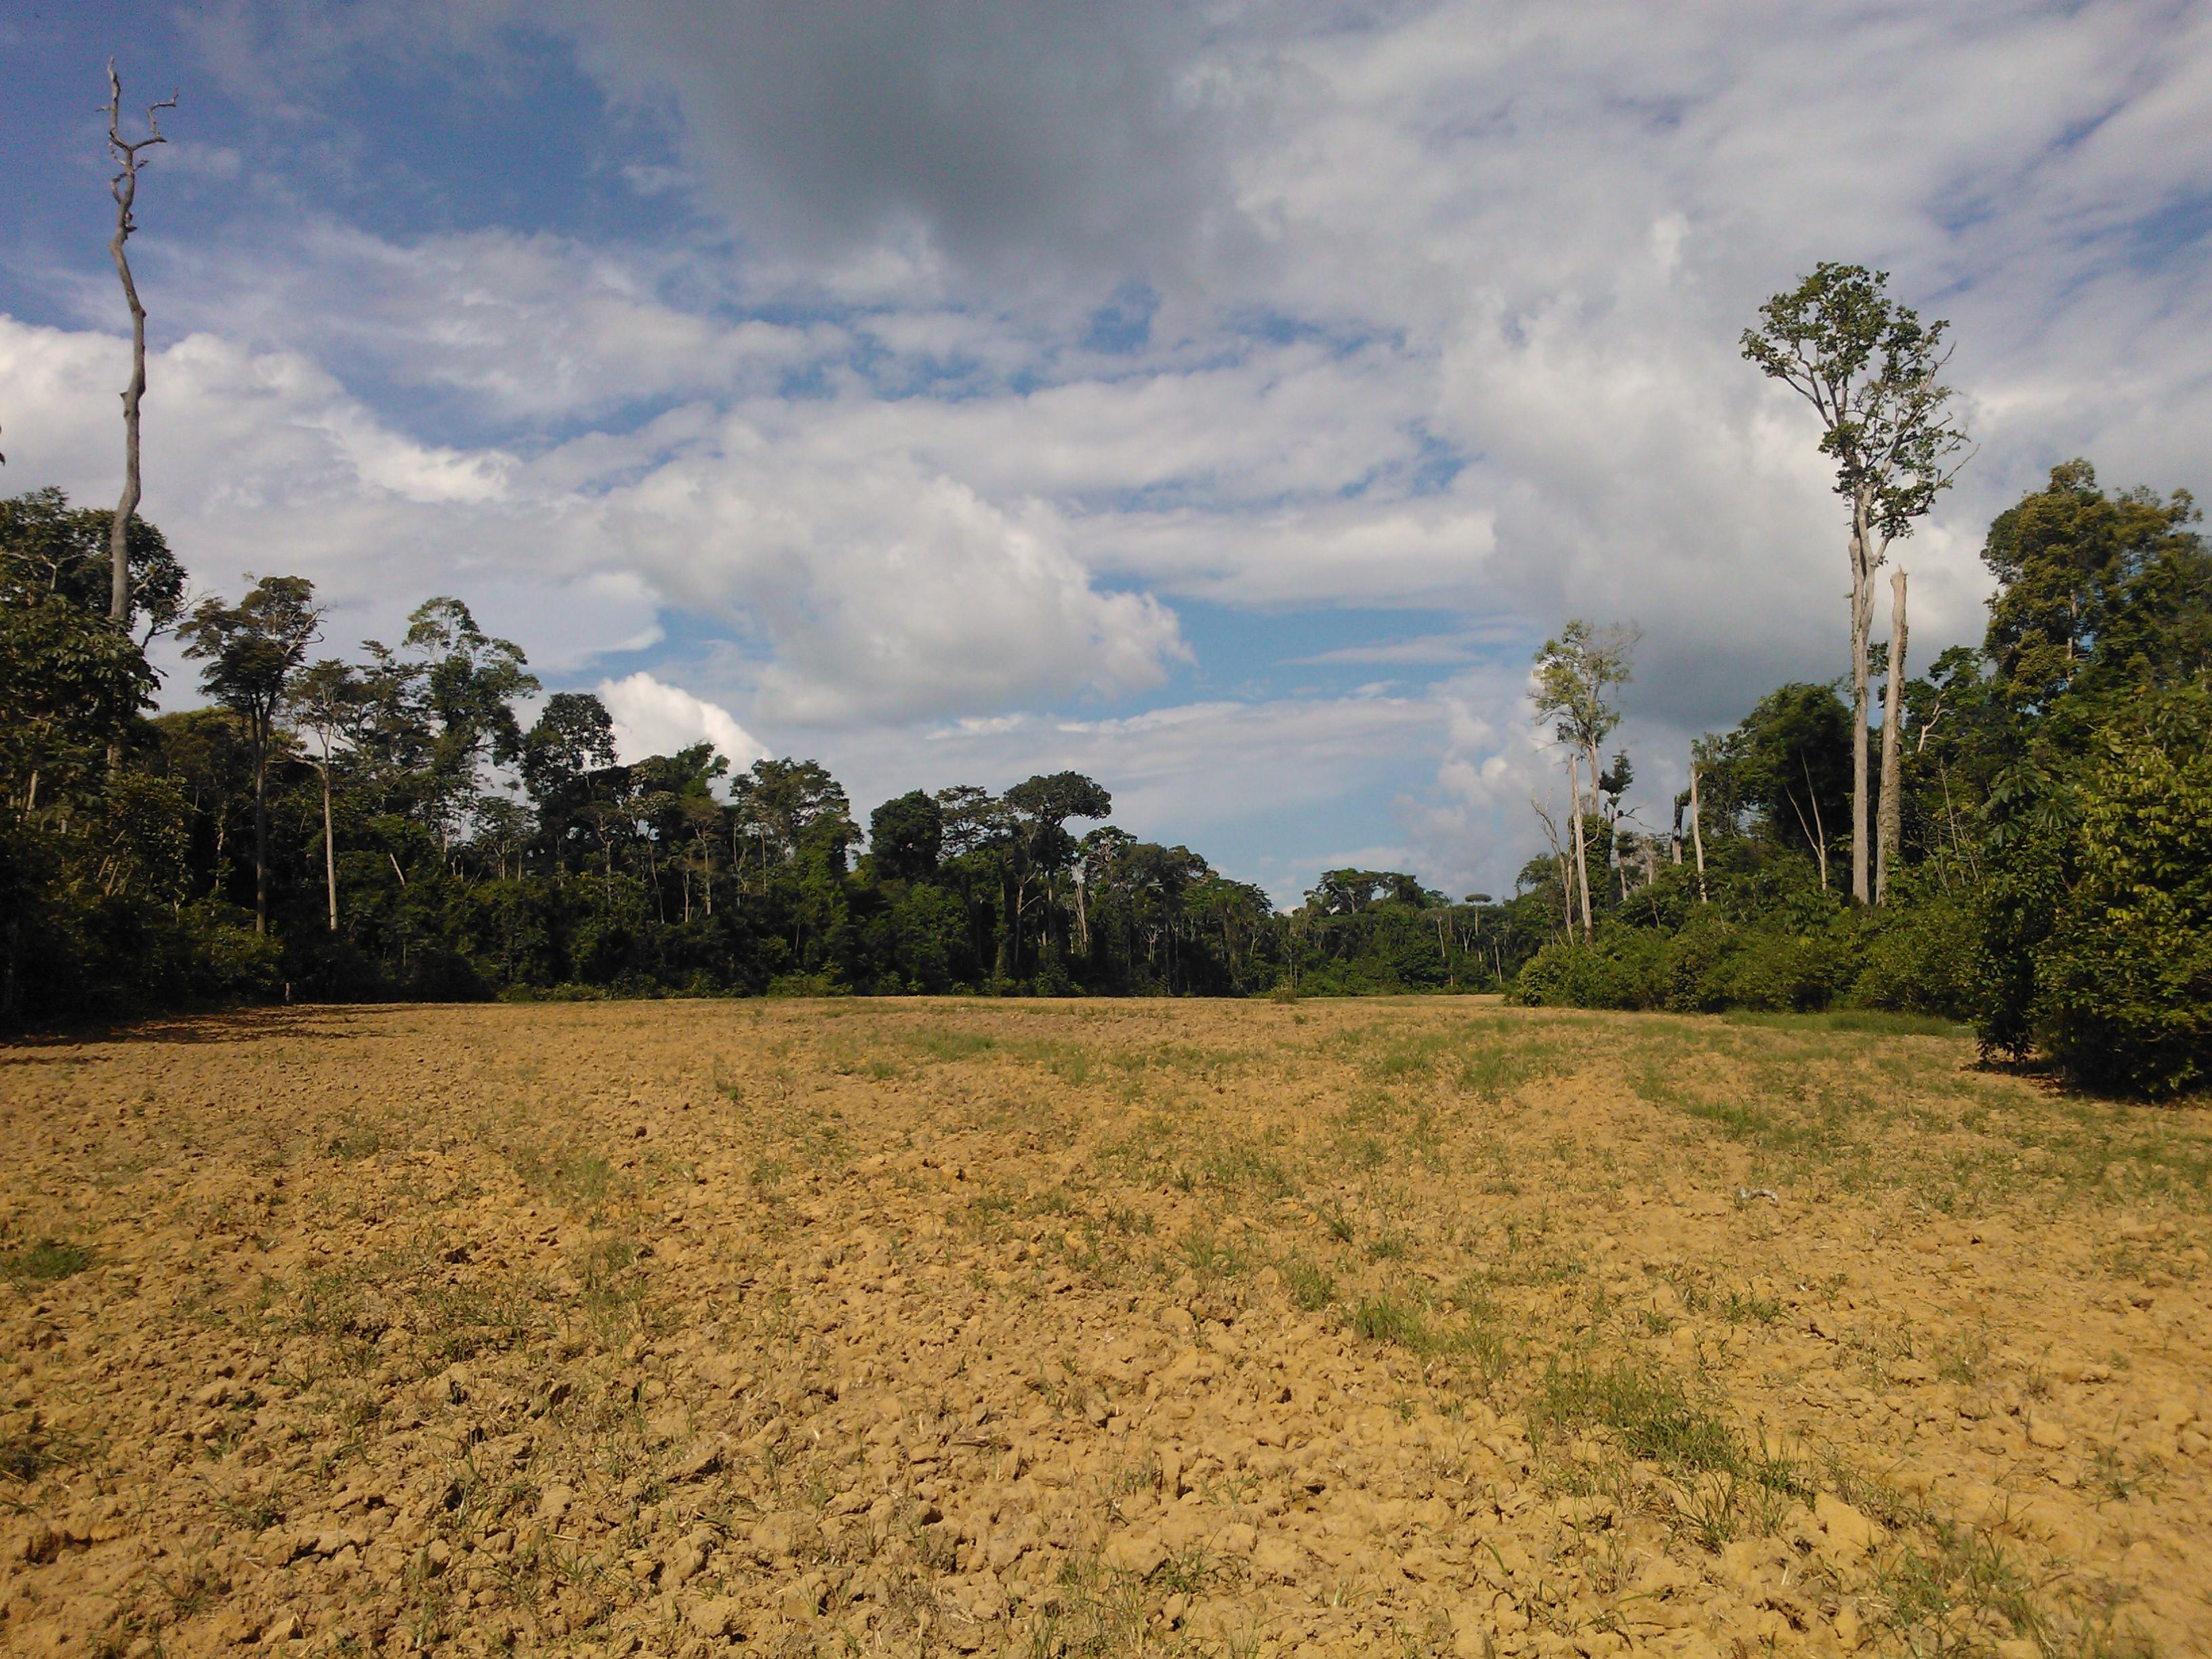
\includegraphics[width=0.495\textwidth]{figuras/resultados/small_modis_right.png}
\caption{Imagem de solo exposto. � esquerda, uma imagem selecionada e uma pequena janela com suas propriedades. � direita imagem capturada exibida em maior resolu��o. No mapa, uma camada MODIS ativa.}
\label{map:small_selected_modis_right}
\end{figure}

Ambas imagens (Fig. \ref{map:small_selected_modis_left} e \ref{map:small_selected_modis_right}) tornam evidente tratar-se de �rea n�o florestada. Por�m, utilizando-se apenas a imagem MODIS (Fig. \ref{map:small_map_modis}) falta resolu��o para se obter uma classifica��o precisa, mesmo com uma inspe��o visual feita por um volunt�rio.

\begin{figure}[h]
\centering
\includegraphics[width=0.8\textwidth]{figuras/resultados/small_map_spot.png}
\caption{� esquerda, uma imagem selecionada e uma pequena janela com suas propriedades. � direita imagem capturada exibida em maior resolu��o. No mapa, uma camada SPOT ativa.}
\label{map:small_map_spot}
\end{figure}

Observando as propriedades das imagens Fig. \ref{map:small_selected_modis_left} e Fig. \ref{map:small_selected_modis_right}, � poss�vel notar uma propriedade interessante. A orienta��o das imagens condiz perfeitamente com a vis�o do mapa mostrado na Figura \ref{map:small_map_spot}, uma vez que essas foram capturadas logo no in�cio do pol�gono desflorestado, e n�o no interior do mesmo. Assim, � poss�vel observar que a fun��o da b�ssola � muito importante pois esta fornece em qual dire��o a foto foi realizada. Caso a dire��o estivesse errada, a seta poderia mostrar para uma parte florestada e exibir uma imagem n�o florestada. Ao treinar uma algoritmo supervisionado, este poderia apresentar diverg�ncia por causa deste valor, assumindo que fosse 100\% correto.

Resumindo, a exist�ncia de v�deos e �udios captados por volunt�rios, registrando a fauna local, alguma atividade il�cita de desmatamento, �reas de inc�ndio, sons de tratores, entre outros, pode auxiliar a tarefa de classifica��o autom�tica de uma imagem de sat�lite, servindo, por exemplo, de \textit{feedback} � rede neural, tornando-a uma rede supervisionada.

\section{Conclus�es e Trabalhos Futuros}
\label{ch:conclusoes}

O objetivo deste trabalho foi o de propor, desenvolver e testar um m�dulo de sensoriamento volunt�rio e integr�-lo ao projeto ForestWatchers. A solu��o foi desenvolver um aplicativo h�brido em que volunt�rios que possuam diferentes tipos de dispositivos possam contribuir, captando �udio, v�deo e imagens. Junto com o aplicativo, foi desenvolvido um m�dulo web para exibi��o dos dados.

O aplicativo foi desenvolvido utilizando o \textit{framework} PhoneGap, que permite utilizar um �nico c�digo para gerar aplicativos em outras plataformas de forma f�cil, at� mesmo por linha de comando. O c�digo foi escrito usando a conven��o do PhoneGap (HTML, CSS e JavaScript). Os componentes JQueryMobile e KnockoutJS foram utilizados para desenhar a interface gr�fica do aplicativo. Por�m, antes de concluirmos que o aplicativo deveria ser h�brido, foram testados duas outras solu��es para o desenvolvimento do aplicativo. A primeira, utilizando bibliotecas nativas, exigia que cada aplicativo fosse desenvolvido na sua respectiva plataforma desde o princ�pio. Posteriormente, foi verificado o uso de \textit{frameworks} coleta de dados, como EpiCollect e Sensr como uma solu��o. Por n�o ter controle das funcionalidades e os \textit{frameworks} mais modernos serem desenvolvidos para apenas uma �nica plataforma, esta abordagem foi tamb�m descartada.

O m�dulo de SV aqui desenvolvido obt�m informa��es dos sensores de c�mera (para a captura de imagem e v�deo), microfone (�udio), localiza��o (GPS), orienta��o (b�ssola). Os dados s�o armazenados no dispositivos para serem enviados posteriormente, seguindo um modelo de envio por demanda, quando o usu�rio solicitar. Desta forma, o tr�fico de arquivos grandes como v�deo e �udio podem ser feitos atrav�s de redes WiFi ao inv�s de conex�es 3G.

O back-end web � encarregado de receber os dados enviados pelos volunt�rios e armazen�-los adequadamente nos bancos de dados, assim como enviar os dados solicitados pela interface web (o front-end do m�dulo) para a exibi��o dos resultados. Cada recurso (imagem, �udio ou v�deo) possui sua respectiva coordenada e outras propriedades.

O m�dulo de SV foi desenvolvido utilizando Python e o \textit{micro framework} Flask com suas extens�es, voltado ao desenvolvimento de aplica��es web e comunica��o web. Um servidor de comunica��o web baseado na arquitetura REST foi tamb�m desenvolvido, utilizando o protocolo HTTP.

A interface gr�fica (front-end) exibe os dados e resultados enviados pelos volunt�rios. Esta interface � na forma de uma p�gina web que utiliza-se do mesmo servidor (Flask) do back-end. A p�gina exibe os dados georreferenciados utilizando componentes de mapas.

A interface foi desenvolvida em HTML5, CSS3 e JavaScript. Utilizou-se a biblioteca OpenLayers v2 para posicionar cada recurso em sua coordenada que foi captada e mostrar diversos outros mapas ao fundo, dando o poder ao usu�rio de alternar estes mapas em um sistema de camadas, onde o �ltimo selecionado sobrep�e o primeiro. Por�m, sempre mantendo os recursos por cima. Outros componentes tamb�m foram utilizados na confec��o desta p�gina web, como o \textit{framework} de HTML5 Twitter Bootstrap na sua vers�o 3, permitindo de forma r�pida e f�cil a cria��o de sistemas de \textit{grid} para o posicionamento de conte�do, janelas modais e de intera��es, menus e barras para navega��o. Por �ltimo, o componente Sly foi utilizado para mostrar miniaturas dos recursos retornado pelo m�dulo web, facilitando a itera��o do usu�rio com os dados a serem visualizados. Este tamb�m permite acesso por toque, sendo imprescind�vel no uso para \textit{tablets} e \textit{smartphones}, dispositivos capazes de toque.

Para testar o m�dulo proposto neste trabalho, o aplicativo foi utilizado em uma �rea do Estado do Par�, pr�ximo a Belterra. O aplicativo captou fotos e v�deo para serem sincronizados posteriormente com o m�dulo web. Nesta etapa, n�o foi poss�vel validar o sistema de captura de �udio devido a um erro no c�digo encontrado na vers�o do PhoneGap para o sistema Windows Phone e por a �rea n�o possuir comunica��o com internet. Os dados apresentados neste trabalho para o �udio s�o representativos e foram gerados a partir da extra��o do �udio dos arquivos de v�deos captados.

Como trabalhos futuros, pretende-se integrar ao m�dulo outros tipos de dados. Existem diversos s�tios que permitem compartilhar dados de sensores ambientais pela internet\footnote{\url{https://thingspeak.com}}. Estuda-se agregar tais dados ao projeto permitindo uma vis�o geral do meio ambiente.

Outro grande avan�o esperado para o projeto, � o estudo de como pode ser aumentado a confiabilidade dos dados capturados pelos volunt�rios. Ferramentas adicionais ser�o estudas para evitar a falsifica��o de dados captadas e o uso de inadequado do aplicativo.

E por fim, ser� avaliado uma forma de adicionar formul�rios aos aplicativo, de forma an�loga ao sistema apresentado pelo EpiCollect. Possibilitando que novos projetos possam utilizar o aplicativo h�brido aqui desenvolvido para coletar dados tabulados, utilizando regras e op��es j� definidas para o seu cadastro, conforme foi utilizado pelos alunos que auxiliaram a DPI do INPE na �rea de estudo.

%% %% + Breve discuss�o
\chapter{INTRODU��O}
%% \chapter{REVIS�O BIBLIOGR�FICA}

\section{Sistemas de Monitoramento de Desmatamento}
\subsection{PRODES}
\subsection{DETER}

\section{Ci�ncia Cidad�}
\subsection{Defini��o}
\subsection{Hist�rico}
\subsection{Avan�os na Ci�ncia}
\subsection{Suas Formas}
\subsubsection{Projetos}

\section{Sistemas de Monitoramento Ambientais Colaborativos}
\subsection{Projetos}

\section{ForestWatchers}
\subsection{Proposta}
\subsection{Metodologia}
\subsection{Resultados}

\section{Aplicativos M�veis}
\subsection{Surgimento}
\subsection{Divis�o de Mercado}
\subsection{Aplicativos Nativos}
\subsection{Aplicativos H�bridos}





%% %% ++ Desenvolvimento do Aplicativo
%% ++ Capta��o dos Dados
\chapter{METODOLOGIA}
\section{Desenvolvimento do Aplicativo}
\section{Capta��o dos Dados}
%% \chapter{RESULTADOS E DISCUSS�ES}
% \appendix
\bibliography{./bib/publicacao_nova} %% aponte para seu arquivo de bibliografia no formato bibtex (p.ex: referencia.bib)
\inicioApendice
%%%%%%%%%%%%%%%%%%%%%%%%%%%%%%%%%%%%%%%%%%%%%%%%%%%%%%
%Ap�ndice A
\hypertarget{estilo:apendice1}{} %% uso para este Guia
%Este ap�ndice foi criado apenas para indicar como construir um ap�ndice no estilo, n�o existia no original da tese.
%%%%%%%%%%%%%%%%%%%%%%%%%%%%%%%%%%%%%%%%%%%%%%%%%%%%%%
\renewcommand{\thechapter}{}%
\chapter{AP�NDICE A - ESTRUTURA \textit{JSON} PARA ENVIO DE ARQUIVOS.}  % trocar A por B na pr�xima ap�ndice e etc
\label{apendice1} % trocar A por B na pr�xima ap�ndice e etc
\renewcommand{\thechapter}{A}%    % trocar A por B na pr�xima ap�ndice e etc

\begin{lstlisting}[language=json,firstnumber=1, caption={Estrutura JSON para envio de um arquivo do tipo de imagem.},captionpos=b, label={json:estrutura_imagem}]
{
  "entry": {
      "picture": {
      "filename" : "",
      "filepath" :  ""
    },
    "compass": {
      "magneticHeading": "",
      "trueHeading": "",
      "orientation": "",
      "useManual": "",
      "accuracy" : "",
    },
    "gps": {
      "latitude": "",
      "longitude": "",
      "accuracy": "",
      "altitude": "",
      "altitudeAccuracy": "",
      "heading": "",
      "speed": ""
    },
    "options": {
      "gpsOptions": {
        "enableHighAccuracy": "",
        "maximumAge": "",
        "timeout": ""
      },
      "compassOptions": {
        "frequency": "",
        "enabled": ""
      },
      "pictureOptions": {
        "quality": ""
      }
    }
  },
  "device": {
    "uuid": "",
    "version": "",
    "cordova": "",
    "platform": "",
    "model": ""
  }
}
\end{lstlisting}


%Este ap�ndice foi criado apenas para indicar como construir um ap�ndice no estilo, n�o existia no original da tese.
%%%%%%%%%%%%%%%%%%%%%%%%%%%%%%%%%%%%%%%%%%%%%%%%%%%%%%
\renewcommand{\thechapter}{}%
\chapter{AP�NDICE B - REQUISI��O E RESPOSTA DO PROTOCOLO HTTP}
\renewcommand{\thechapter}{B}%    % trocar A por B na pr�xima ap�ndice e etc
\label{apendice2} % trocar A por B na pr�xima ap�ndice e etc

\begin{lstlisting}[language=json,firstnumber=1, caption={Uma requisi��o de um recurso HTTP atrav�s do m�todo \textit{GET}. Ao abrir um novo s�tio eletr�nico, todos os navegadores enviam uma solicita��o da p�gina principal neste formato. De mesma forma, um cabe�alho neste formato ser� enviado para os m�todos \textit{POST}, \textit{PUT} e \textit{DELETE}, m�todos b�sicos do protocolo HTTP.}, label={http:inpe_request},captionpos=b]
GET /pos_graduacao/cursos/cap/index.php HTTP/1.1
Host: www.inpe.br
Accept: text/html,application/xhtml+xml
Accept-Encoding: gzip, deflate, sdch
Accept-Language: en-US,en;q=0.8,pt-BR;q=0.6,pt;q=0.4
\end{lstlisting}

% float,floatplacement=H,
\begin{lstlisting}[language=json,firstnumber=1, caption={Resposta a uma requisi��o HTTP de m�todo \textit{GET}. Nesta resposta, o servidor retorna todos os dados referentes ao recurso solicitado. Em caso de arquivos, uma resposta ser� enviada em bin�rio.}, label={http:inpe_response},captionpos=b]
HTTP/1.1 200 OK
Server: Apache/2.2.3 (CentOS)
X-Powered-By: PHP/5.1.6
Content-Type: text/html; charset=iso-8859-1
\end{lstlisting}

\begin{table}[h]
\centering
\small
\caption{M�todos Padr�es do Protocolo HTTP}
\label{tab:metodos_http}
\resizebox{\textwidth}{!}{%
\begin{tabular}{@{}lll@{}}
\toprule
M�todo HTTP & Descri��o da A��o                                                             & Exemplo de Fun��o                                                                                                             \\ \midrule
GET         & \begin{tabular}[t]{@{}l@{}}Obter informa��es \\ sobre um recurso\end{tabular} & \begin{tabular}[t]{@{}l@{}}http://servidor.com/imagens\\ (listar todas as imagens)\end{tabular}                                \\
GET         & \begin{tabular}[t]{@{}l@{}}Obter informa��es \\ sobre um recurso\end{tabular} & \begin{tabular}[t]{@{}l@{}}http://servidor.com/imagem/10\\ (listar a imagem de \\ identifica��o \#10)\end{tabular}             \\
POST        & Criar um novo recurso                                                         & \begin{tabular}[t]{@{}l@{}}http://servidor.com/imagens\\ (criar um novo objeto imagem)\end{tabular}                            \\
PUT         & Atualizar um recurso                                                          & \begin{tabular}[t]{@{}l@{}}http://servidor.com/imagem/10\\ (atualizar os dados da imagem\\ de identifica��o \#10)\end{tabular} \\
DELETE      & Remover um recurso                                                            & \begin{tabular}[t]{@{}l@{}}http://servidor.com/imagem/10\\ (remover o objeto imagem \\ de identifica��o \#10)\end{tabular}     \\ \bottomrule
\end{tabular}
}
\end{table}

\inicioIndice
%%%%%%%%%%%%%%%%%%%%%%%%%%%%%%%%%%%%%%%%%%%%%%%%%%%%%%
%Contracapa
%%%%%%%%%%%%%%%%%%%%%%%%%%%%%%%%%%%%%%%%%%%%%%%%%%%%%%

\thispagestyle{empty}
 \begin{table}
  \begin{center}
  \begin{tabularx}{\textwidth}{X}
   \textbf{PUBLICA��ES T�CNICO-CIENT�FICAS EDITADAS PELO INPE}
  \end{tabularx} 
  \end{center}
 \end{table}
  
 \begin{table}
  \begin{center}
  \begin{tabularx}{\textwidth}{X X}
      
  \textbf{Teses e Disserta��es (TDI)}              & \textbf{Manuais T�cnicos (MAN)}\\
\\
Teses e Disserta��es apresentadas nos Cursos de P�s-Gradua��o do INPE.	&
S�o publica��es de car�ter t�cnico que incluem normas, procedimentos, instru��es e orienta��es.\\
\\
\textbf{Notas T�cnico-Cient�ficas (NTC)}           & \textbf{Relat�rios de Pesquisa (RPQ)}\\
\\
Incluem resultados preliminares de pesquisa, descri��o de equipamentos, descri��o e ou documenta��o de programas de computador, descri��o de sistemas e experimentos, apresenta��o de testes, dados, atlas, e documenta��o de projetos de engenharia. 
&	
Reportam resultados ou progressos de pesquisas tanto de natureza t�cnica quanto cient�fica, cujo n�vel seja compat�vel com o de uma publica��o em peri�dico nacional ou internacional.\\
\\
\textbf{Propostas e Relat�rios de Projetos (PRP)}	& \textbf{Publica��es Did�ticas (PUD)} 
\\
\\
S�o propostas de projetos t�cnico-cient�ficos e relat�rios de acompanhamento de projetos, atividades e conv�nios.
&	
Incluem apostilas, notas de aula e manuais did�ticos. \\
\\         
\textbf{Publica��es Seriadas} 	& \textbf{Programas de Computador (PDC)}\\
\\
S�o os seriados t�cnico-cient�ficos: boletins, peri�dicos, anu�rios e anais de eventos (simp�sios e congressos). Constam destas publica��es o Internacional Standard Serial Number (ISSN), que � um c�digo �nico e definitivo para identifica��o de t�tulos de seriados. 
&	
S�o a seq��ncia de instru��es ou c�digos, expressos em uma linguagem de programa��o compilada ou interpretada, a ser executada por um computador para alcan�ar um determinado objetivo. Aceitam-se tanto programas fonte quanto os execut�veis.\\
\\
\textbf{Pr�-publica��es (PRE)} \\
\\
Todos os artigos publicados em  peri�dicos, anais e como cap�tulos de livros. \\                 \end{tabularx}
  \end{center}
 \end{table}


%\todos
\end{document}
